\documentclass[conference]{IEEEtran}
\IEEEoverridecommandlockouts
% The preceding line is only needed to identify funding in the first footnote. If that is unneeded, please comment it out.
\usepackage{cite}
\usepackage{amsmath,amssymb,amsfonts}
\usepackage{algorithmic}
\usepackage{graphicx}
\usepackage{textcomp}
\usepackage{xcolor}
\def\BibTeX{{\rm B\kern-.05em{\sc i\kern-.025em b}\kern-.08em
    T\kern-.1667em\lower.7ex\hbox{E}\kern-.125emX}}
\begin{document}

\title{Conference Paper Title*\\
{\footnotesize \textsuperscript{*}Note: Sub-titles are not captured in Xplore and
should not be used}
\thanks{Identify applicable funding agency here. If none, delete this.}
}

\author{\IEEEauthorblockN{Deepkumar Patel}
\IEEEauthorblockA{\textit{IMT2021011} \\
\textit{IIIT Bangalore}\\
Bangalore, Karnataka \\
deepkumar.patel@iiitb.ac.in}
\and
\IEEEauthorblockN{Nori Ashish Meher}
\IEEEauthorblockA{\textit{IMT2021085} \\
\textit{IIIT Bangalore}\\
Bangalore, Karnataka \\
meher.ashish@iiitb.ac.in}
\and
\IEEEauthorblockN{Ricky Ratnani}
\IEEEauthorblockA{\textit{IMT2021030} \\
\textit{IIIT Bangalore}\\
Bangalore, Karnataka \\
ricky.ratnani@iiitb.ac.in}
}

\maketitle

\begin{abstract}
This document is a model and instructions for \LaTeX.
This and the IEEEtran.cls file define the components of your paper [title, text, heads, etc.]. *CRITICAL: Do Not Use Symbols, Special Characters, Footnotes, 
or Math in Paper Title or Abstract.
\end{abstract}


\section{SciViz}
\section{Color Mapping}

Color mapping involves assigning colors to data points or regions based on their values. It helps to represent the variations or gradients within a dataset visually. For instance, in our case, different colors represent different wind speeds across the world, allowing viewers to grasp temperature variations quickly.

\subsection{An Important Observation in the Dataset}

% The Dataset We have was the wind speed data from augast to October 2022. Based on our exploration, it's evident that our values typically do not exceed 20, with approximately 99.97\% falling within this range. However, we did encounter a maximum value of around 60, which makes it challenging to fully distinguish values within the 0-20 range.

% say we have  a linear colormap say which is white at 0 and 1 at 60, now since the values are mainly below 20, the values don't take advantage of all the colors and only use about 1/3 of the available color range.
The dataset we possess comprises wind speed data from August to October 2022. Our analysis reveals that, in most cases, the values do not surpass 20, with approximately 99.97\% falling within this threshold. However, we did encounter an outlier with a maximum value of around 60, posing a challenge in effectively distinguishing values within the 0-20 range.

If we employ a linear colormap, where white corresponds to 0 and 1 corresponds to 60, it becomes apparent that the majority of values remain below 20. As a result, these values do not fully utilize the entire color spectrum, utilizing only about one-third of the available color range.

% and this is why we fix a colormap range beforehand and this also helps us when we make a comparison for different days as same color represent the same value in all the visualizations.
This is precisely why we establish a predefined colormap range. This practice also proves advantageous when making comparisons across different days, as consistent colors represent identical values in all the visualizations.

\subsection{Comparing Colormaps}
% for our visualization we use various different types of colourmaps, to be exact, viridis, magma, jet, coolwarm, greys and twilight. Out of this viridis, magma, greys, are sequential. Rest of coolwarm, jet,twilight are diverging. We also used Linear log and discrete distribution for all the colormaps.
In our visualizations, we employ a range of diverse color maps, specifically including viridis, magma, jet, coolwarm, greys, and twilight. Among these, viridis, magma, and greys are classified as sequential color maps, while coolwarm, jet, and twilight fall under the diverging category. Additionally, we apply linear, logarithmic, and discrete distribution techniques across all these color maps.

% Comparing Sequential and Diverging Colormaps, Logically it makes sense to use sequential colormaps as the value is directly proportional to the value in only one direction, and viridis is our favourite in that. but when we look at twilight colormap, it becomes more easier to distinguish between high speed and low speed regions. this is easier to visualize than to explain on paper.

When we contrast \textbf{Sequential and Diverging} Colormaps, it's logical to opt for Sequential Colormaps since the value corresponds directly in one direction. Viridis stands out as our favorite in this category. However, with the twilight colormap, distinguishing between high and low-speed regions becomes notably easier. This visual distinction is more apparent than easily explained on paper.

We have a personal preference for the twilight colormap because it provides a clear visual cue: when the color tends towards red, it signifies a high-speed region, while a shift towards blue indicates a low-speed region.

% When we compare linear, logarithmic and discrete colormaps. We prefer linear and discrete over logarithmic. in case of our data the data lies majority between 0 and 20 and making a logarithmic color palette would lead to most of the values getting very similar colors as seen in the image files. both linear and discrete colormaps are better for making inferences. personally for discrete colormap we divided the color pallets in 10 bins.

In our comparison of \textbf{linear, logarithmic, and discrete} colormaps, our preference leans toward linear and discrete over logarithmic mappings. Given our dataset primarily falls between 0 and 20, a logarithmic color scheme tends to render most values with very similar colors, as observed in the image files. Both linear and discrete colormaps are more effective for drawing inferences. For our discrete colormap, we segmented the color palette into 10 bins, which we found personally effective.

% For comparing colormaps, we see which of them have a diverse color palette, which of them makes it easier to distinguish between high and low wind speed regions,  we also took feedback from our colleagues and then concluded that viridis was the best sequential and twilight was the best diverging colormap.

When evaluating colormaps, we assess their color diversity and their effectiveness in distinguishing between high and low wind speed regions. Additionally, we gather feedback from colleagues to reach a consensus. As a result, our assessment indicates that viridis stands out as the most effective sequential colormap, while twilight is the top choice for diverging colormaps.

\begin{figure}
    \centering
    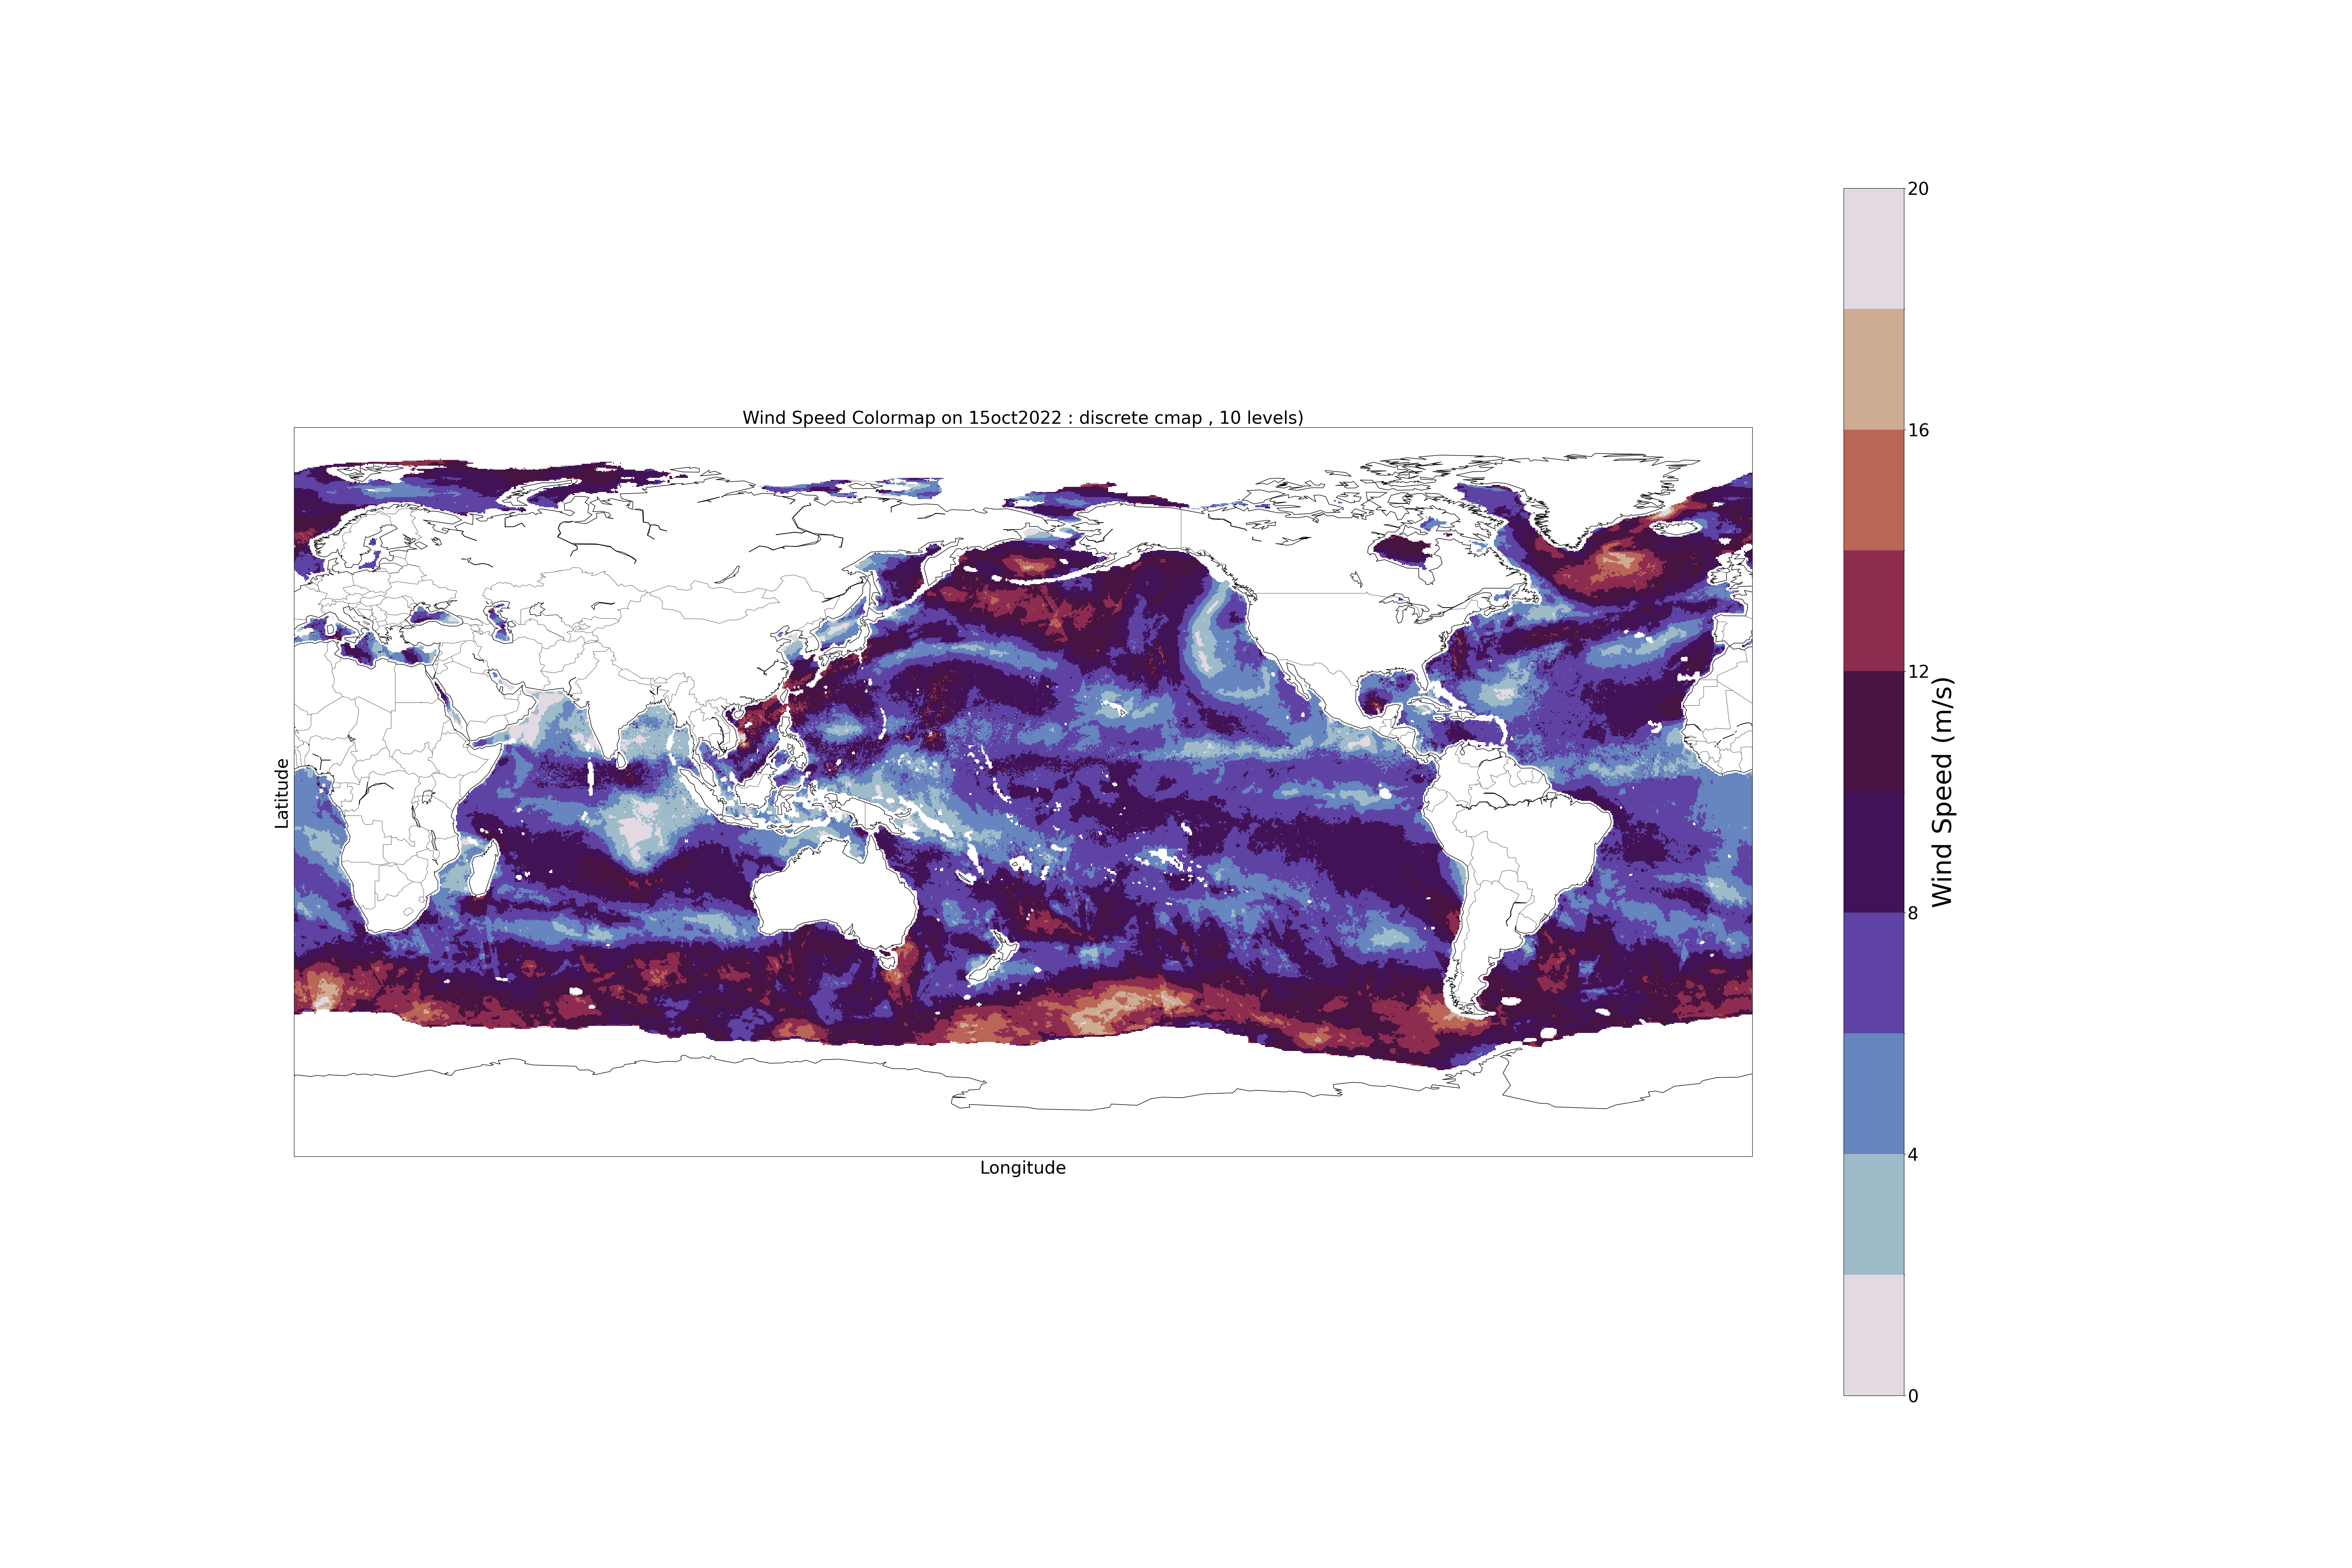
\includegraphics[scale=0.05]{images_deep/twilight_dis.png}
    \caption{Twilight Colormap with Discrete Distribution.}
    \label{colormap_1}
\end{figure}

\begin{figure}
    \centering
    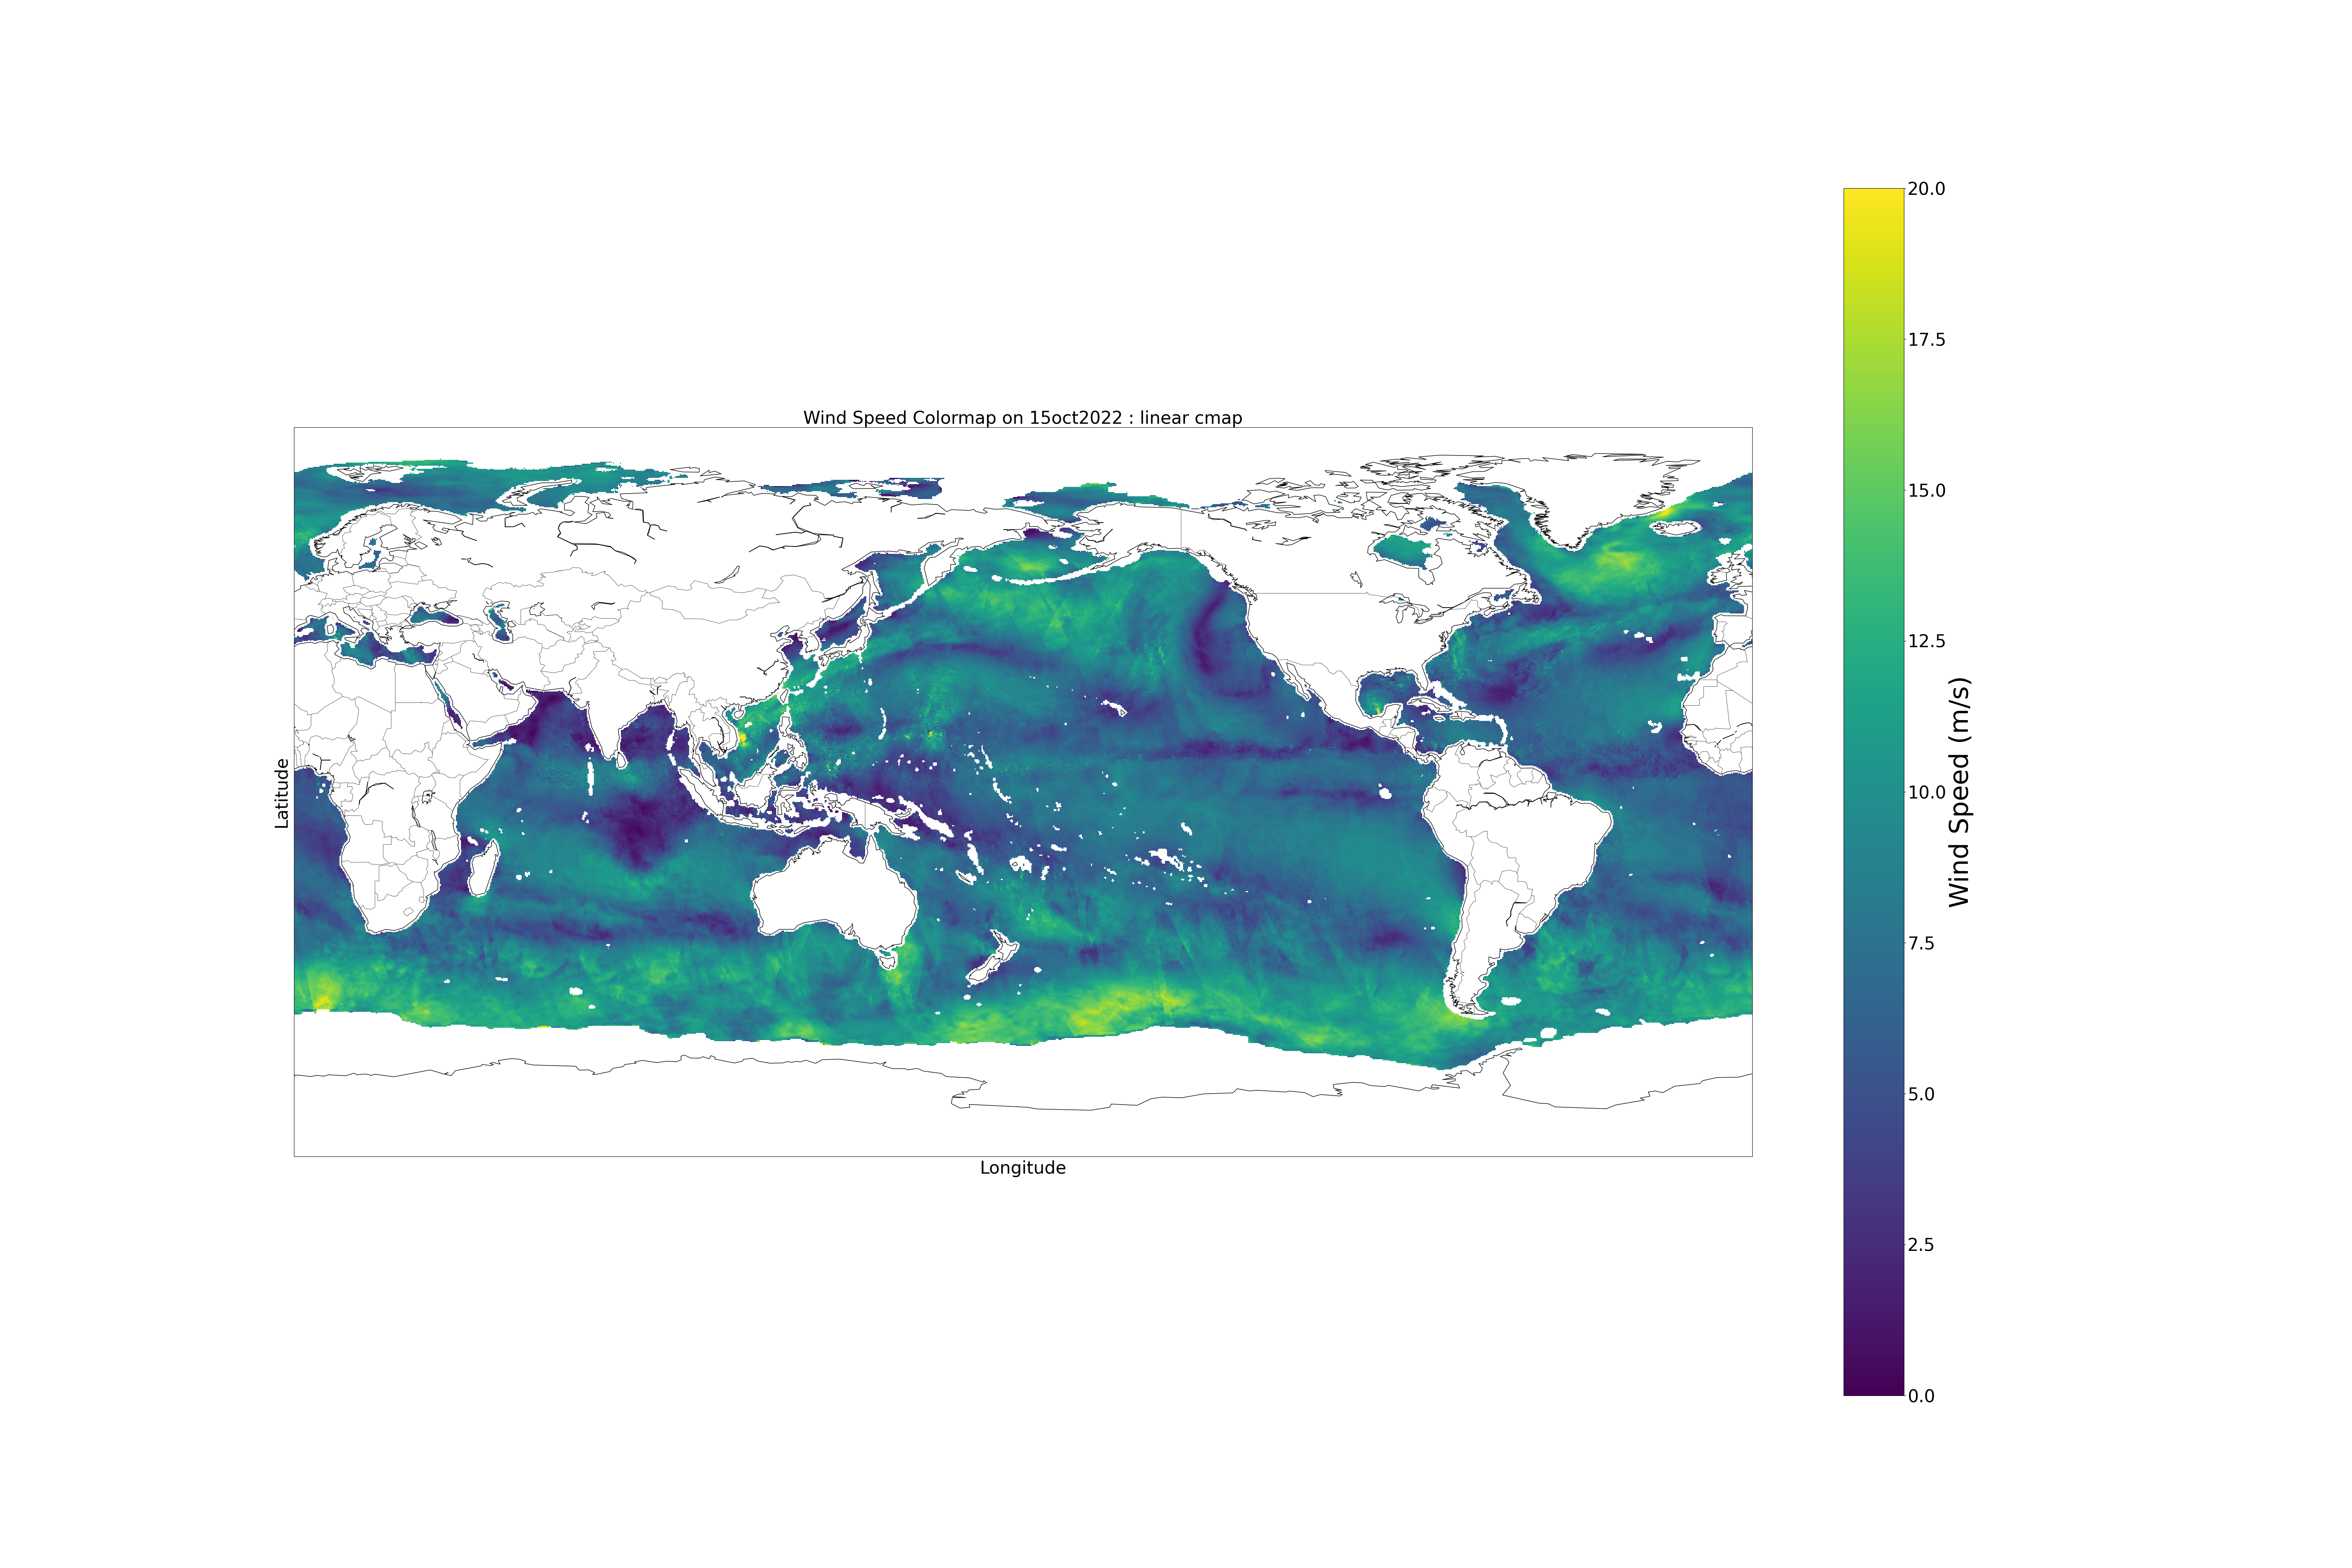
\includegraphics[scale=0.05]{images_deep/viridis_lin.png}
    \caption{Viridis Colormap with Linear Distribution }
    \label{colormap_2}
\end{figure}

\begin{figure}
    \centering
    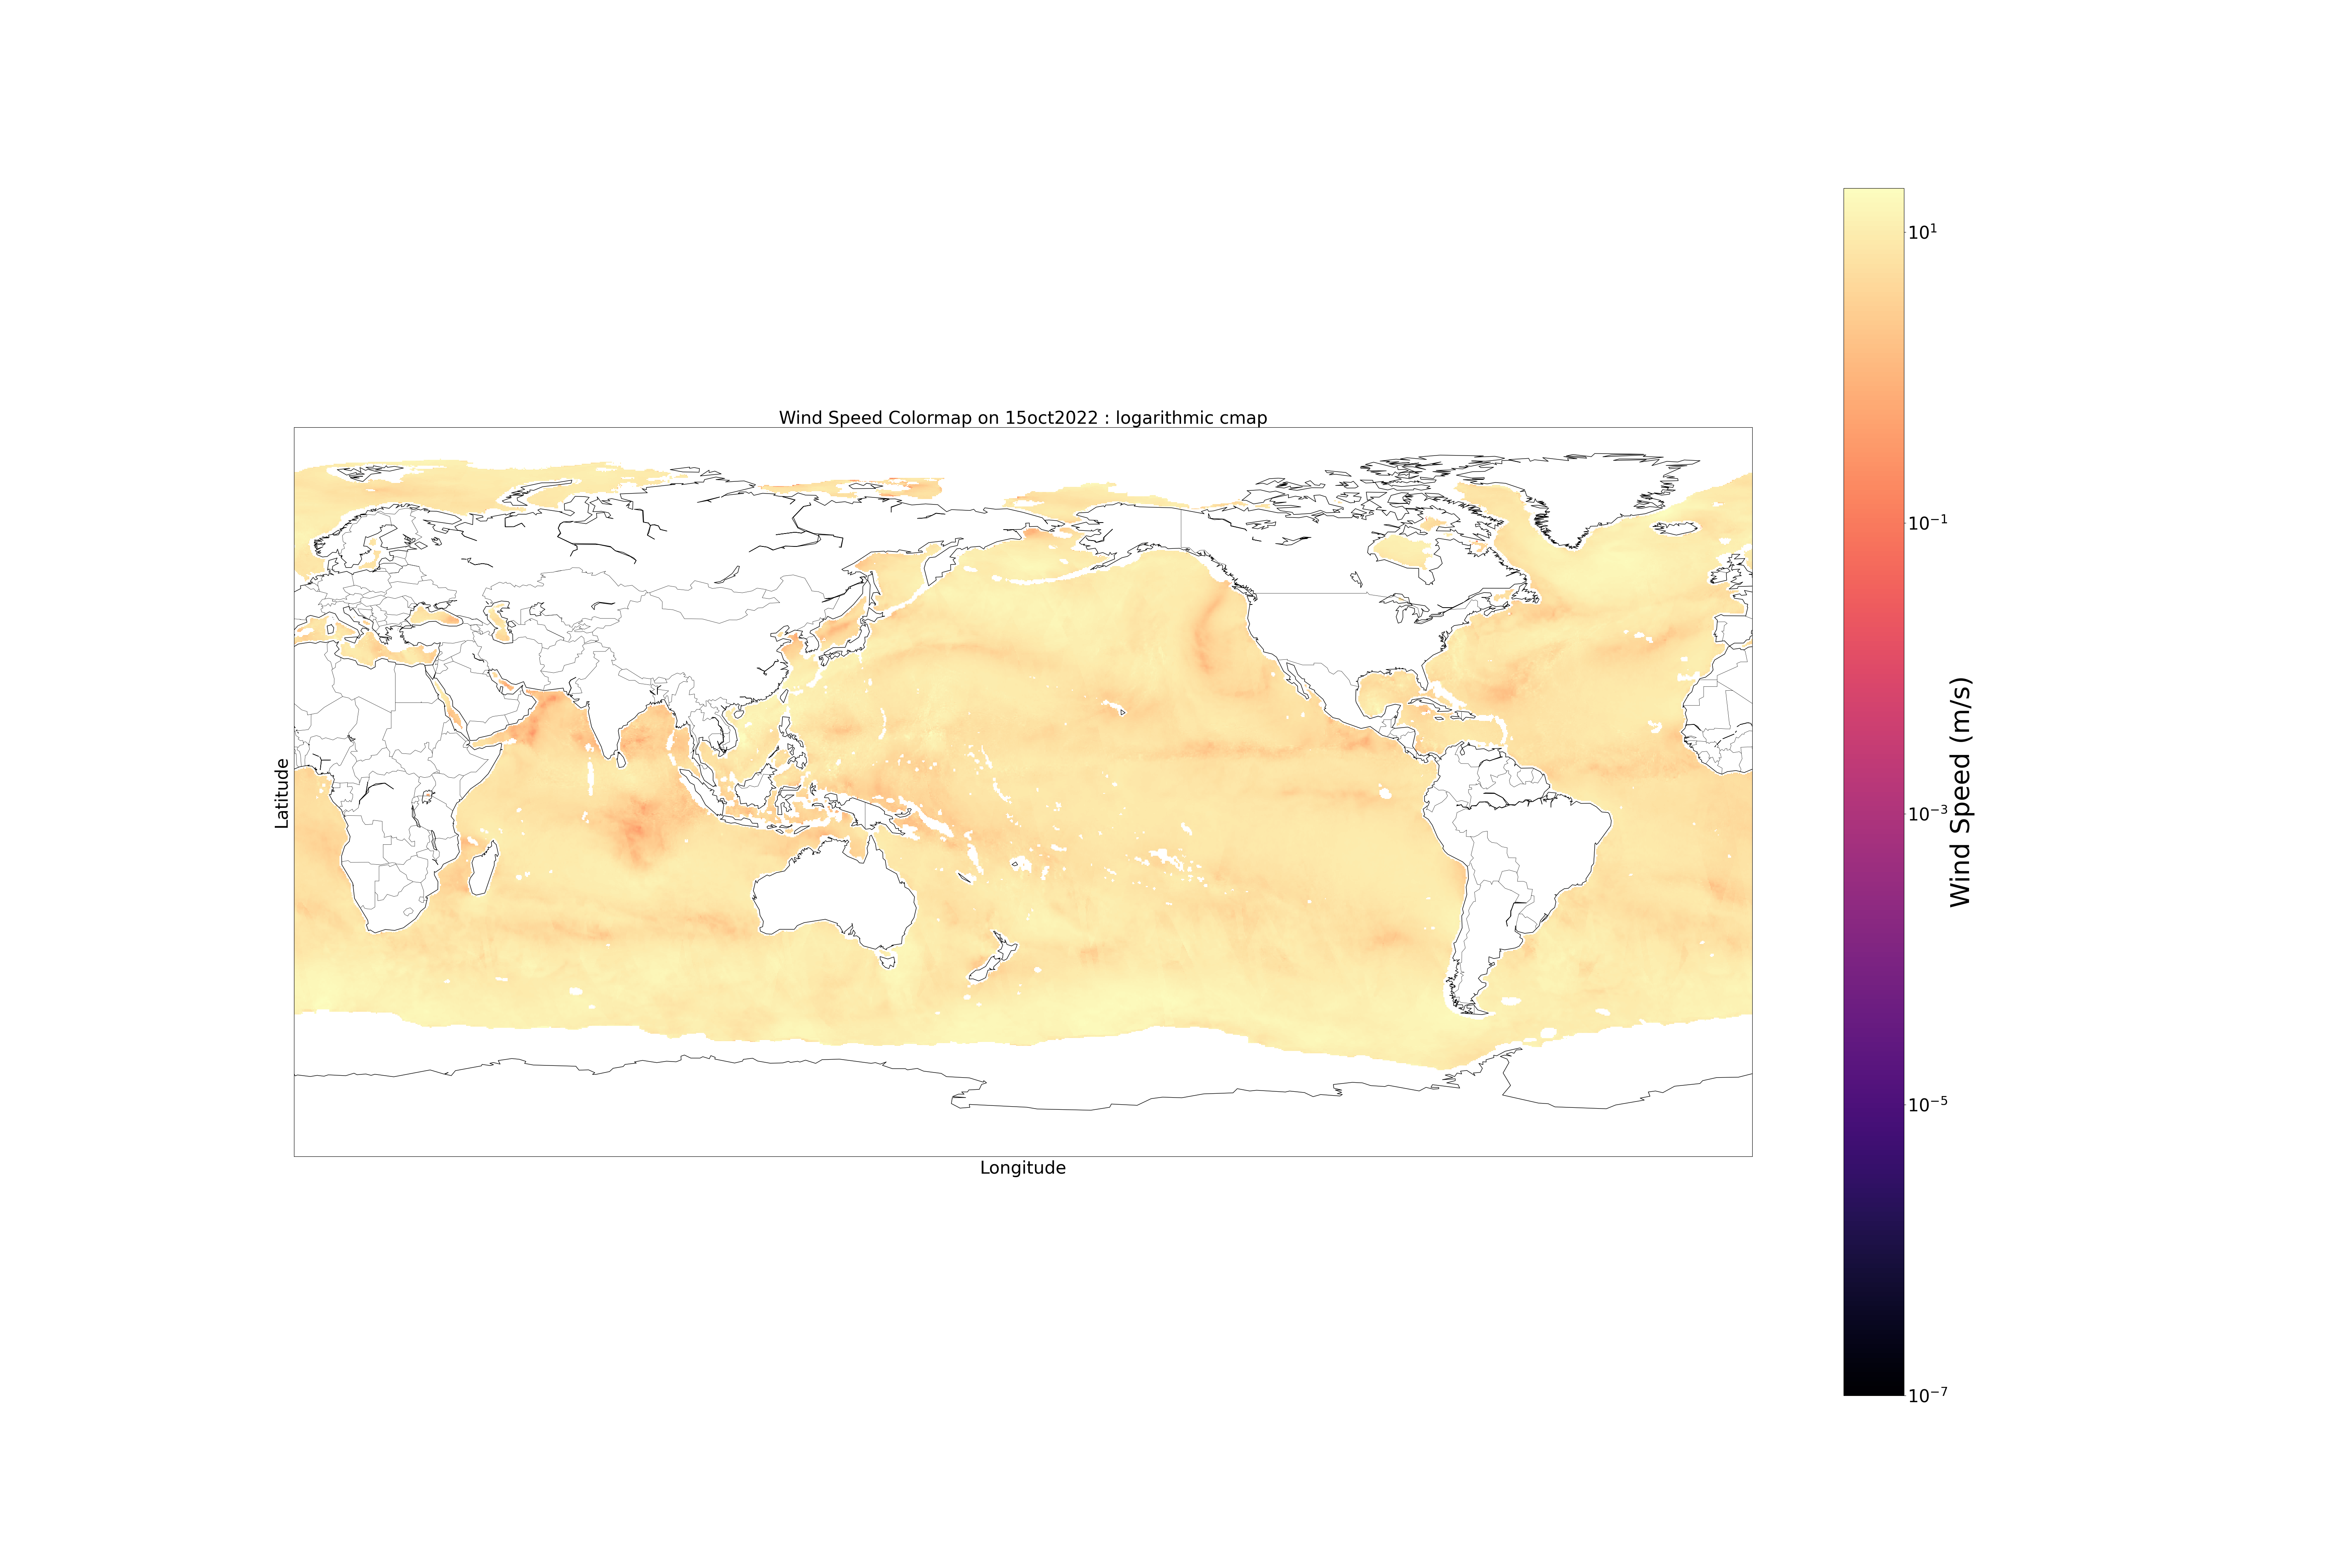
\includegraphics[scale=0.05]{images_deep/magma_log.png}
    \caption{Magma Colormap with Log Distribution. It is not what we prefer.}
    \label{colormap_3}
\end{figure}

\subsection{Observations}
\begin{enumerate}
    \item The windspeed has been generally high in the southern ocean regions throughout April-October.
    
    \item In August, the windspeed in the Indian Ocean displayed a trend of initiating at a high level, undergoing a decline in the first half, and then recovering in the latter half. A similar pattern was observed in another ocean, with an initial high, a decline in the first week, and a subsequent increase in the fourth week of August.

    \item During September, the wind speed commenced at a notably high level but experienced a sudden and sharp decline by September 15th, followed by a subsequent increase for the remainder of the month.

    \item In October, the wind speed steadily rose until late in the month, after which it diminished in the final week of October.
    
\end{enumerate}

\subsection{Cyclone Sitarang}
% Cyclonic Storm Sitrang[a] was a weak tropical cyclone that affected India and Bangladesh in late October 2022. and this is what we detected in our dataset. The images on 19, 23 and 28 October 2022, it can be seen that the wind speed in the bay of bengal near Bangladesh and west bengal, India increased on 23 compared to 19 and then reduced to normal on 28. This observation is related to the clone Sitarang.

Cyclonic Storm Sitrang a was a relatively mild tropical cyclone that had an impact on India and Bangladesh in late October 2022. Our dataset successfully captured this event. When examining the images from October 19, 23, and 28, 2022, it becomes evident that the wind speed in the Bay of Bengal, near Bangladesh and West Bengal, India, escalated on the 23rd in comparison to the 19th and subsequently returned to normal levels by the 28th. This observation is directly connected to Cyclonic Storm Sitrang.

\begin{figure}
    \centering
    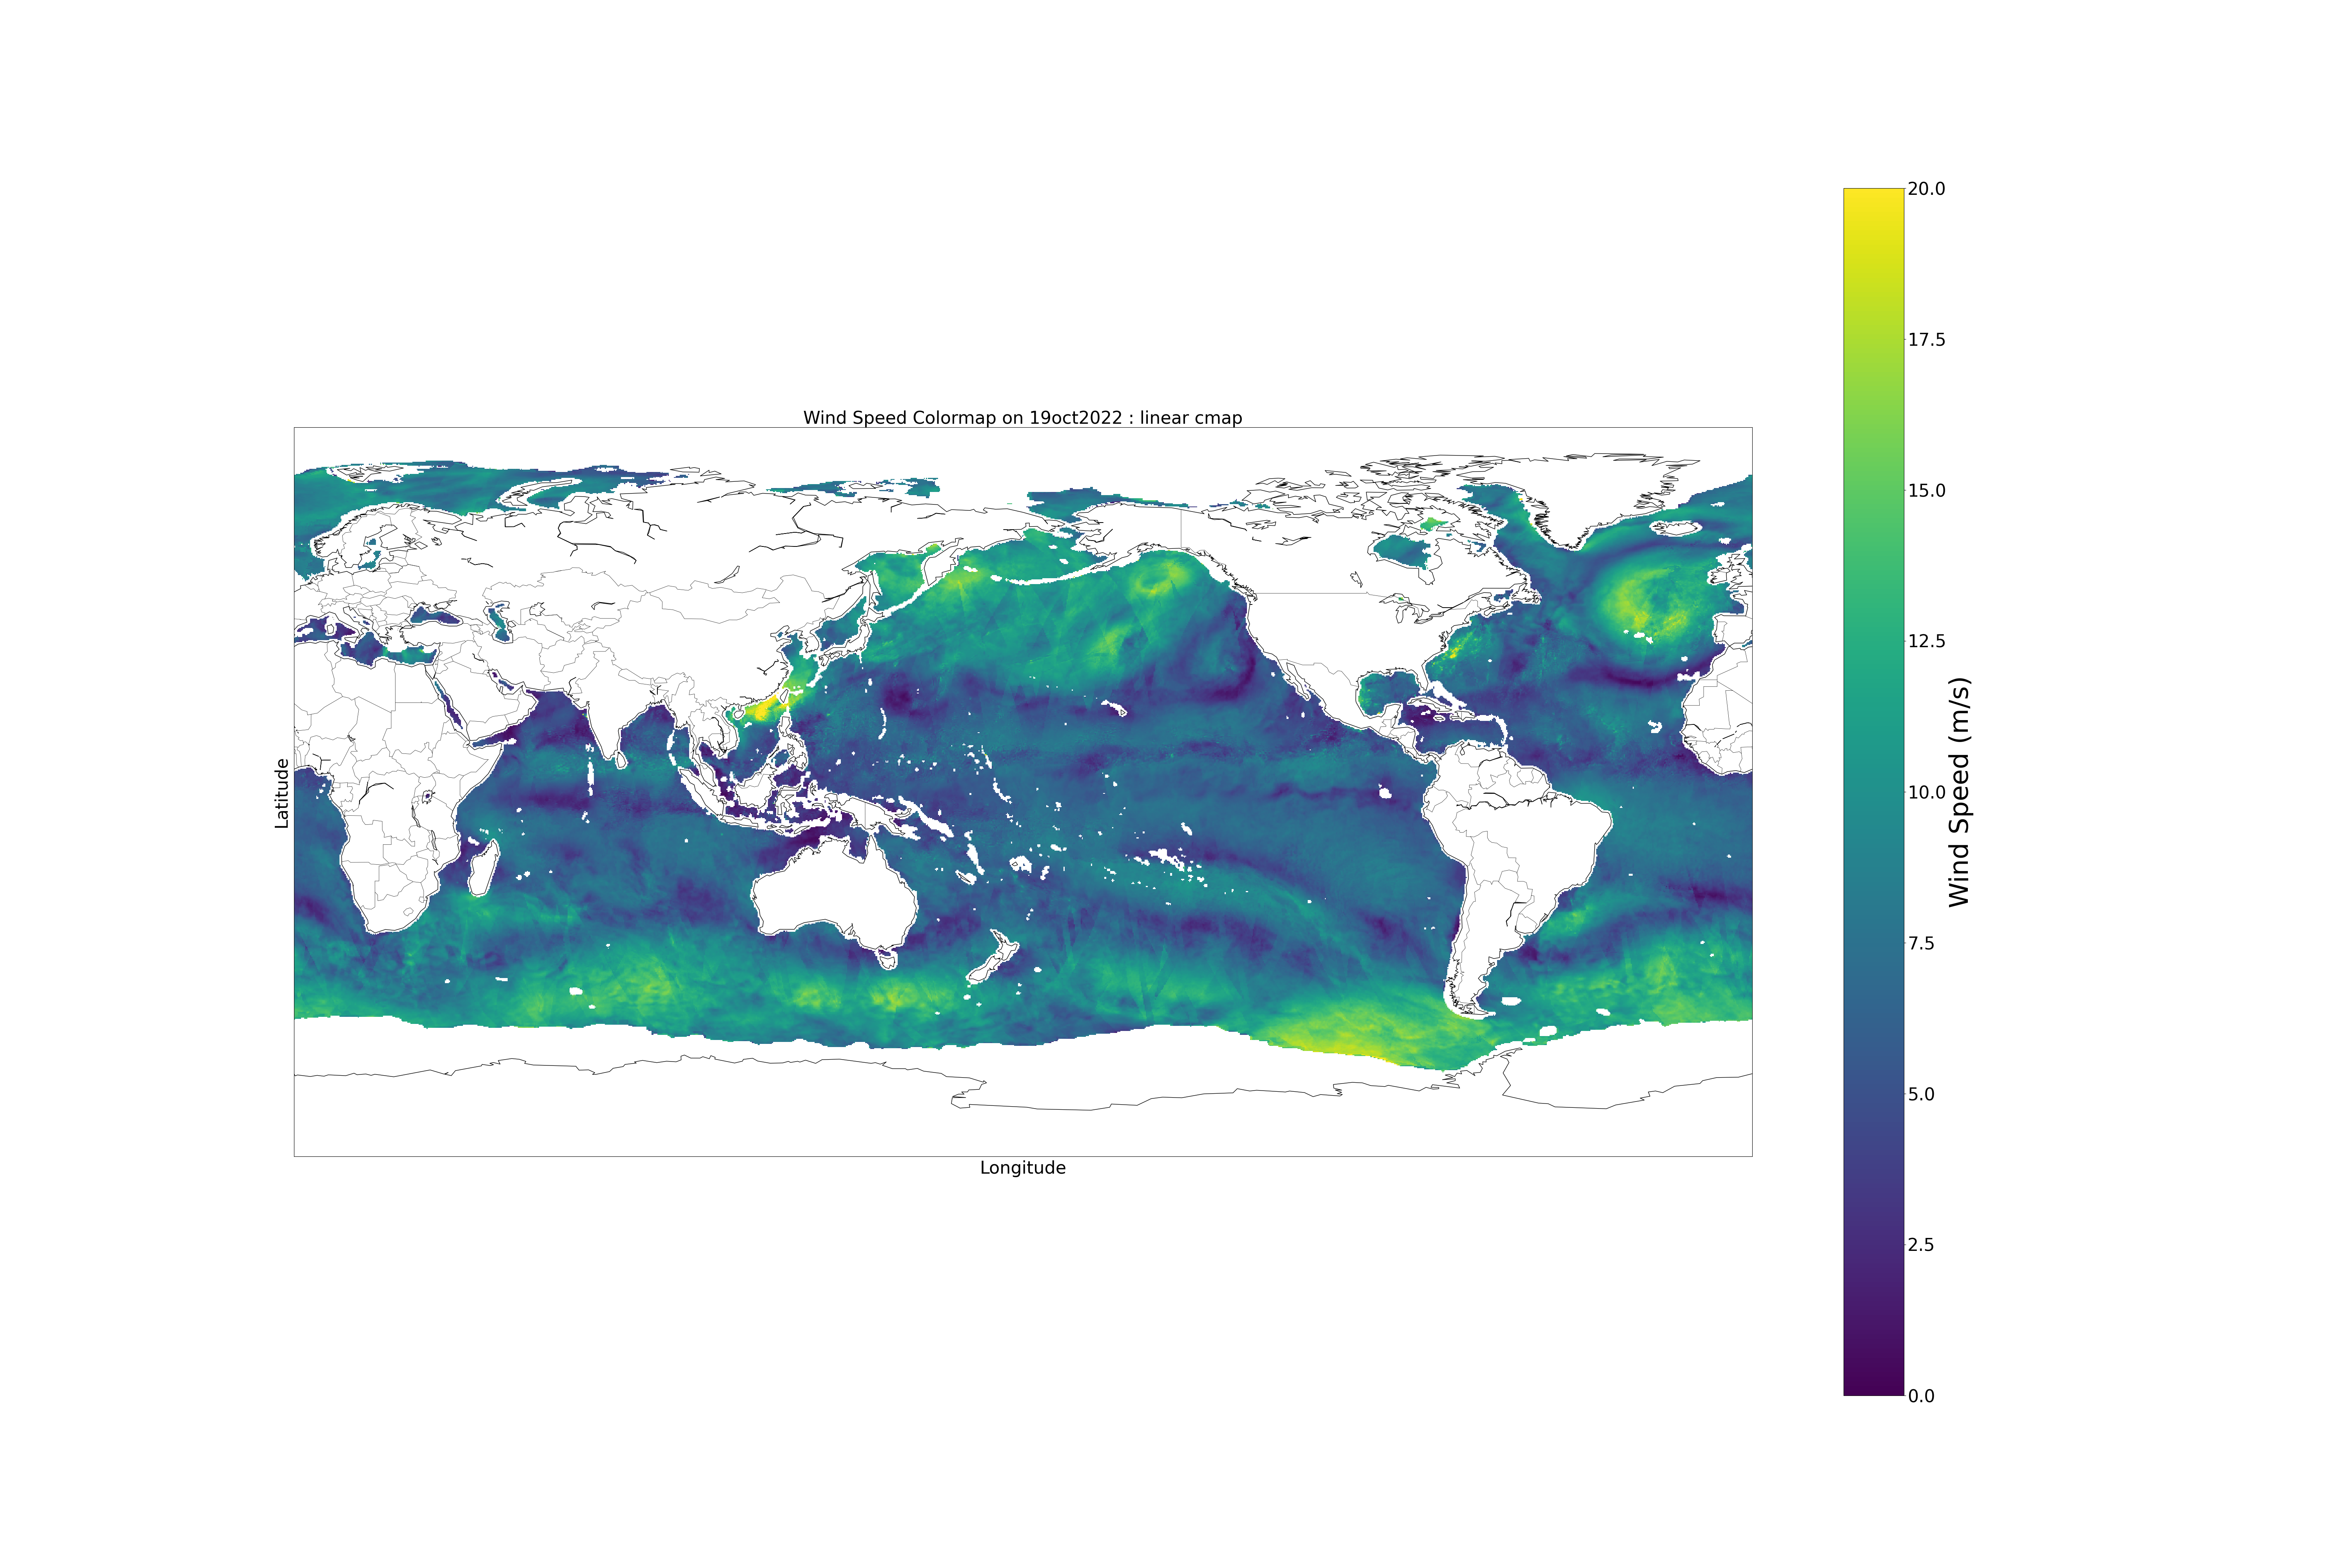
\includegraphics[scale=0.05]{images_deep/viridis_lin_19oct2022.png}
    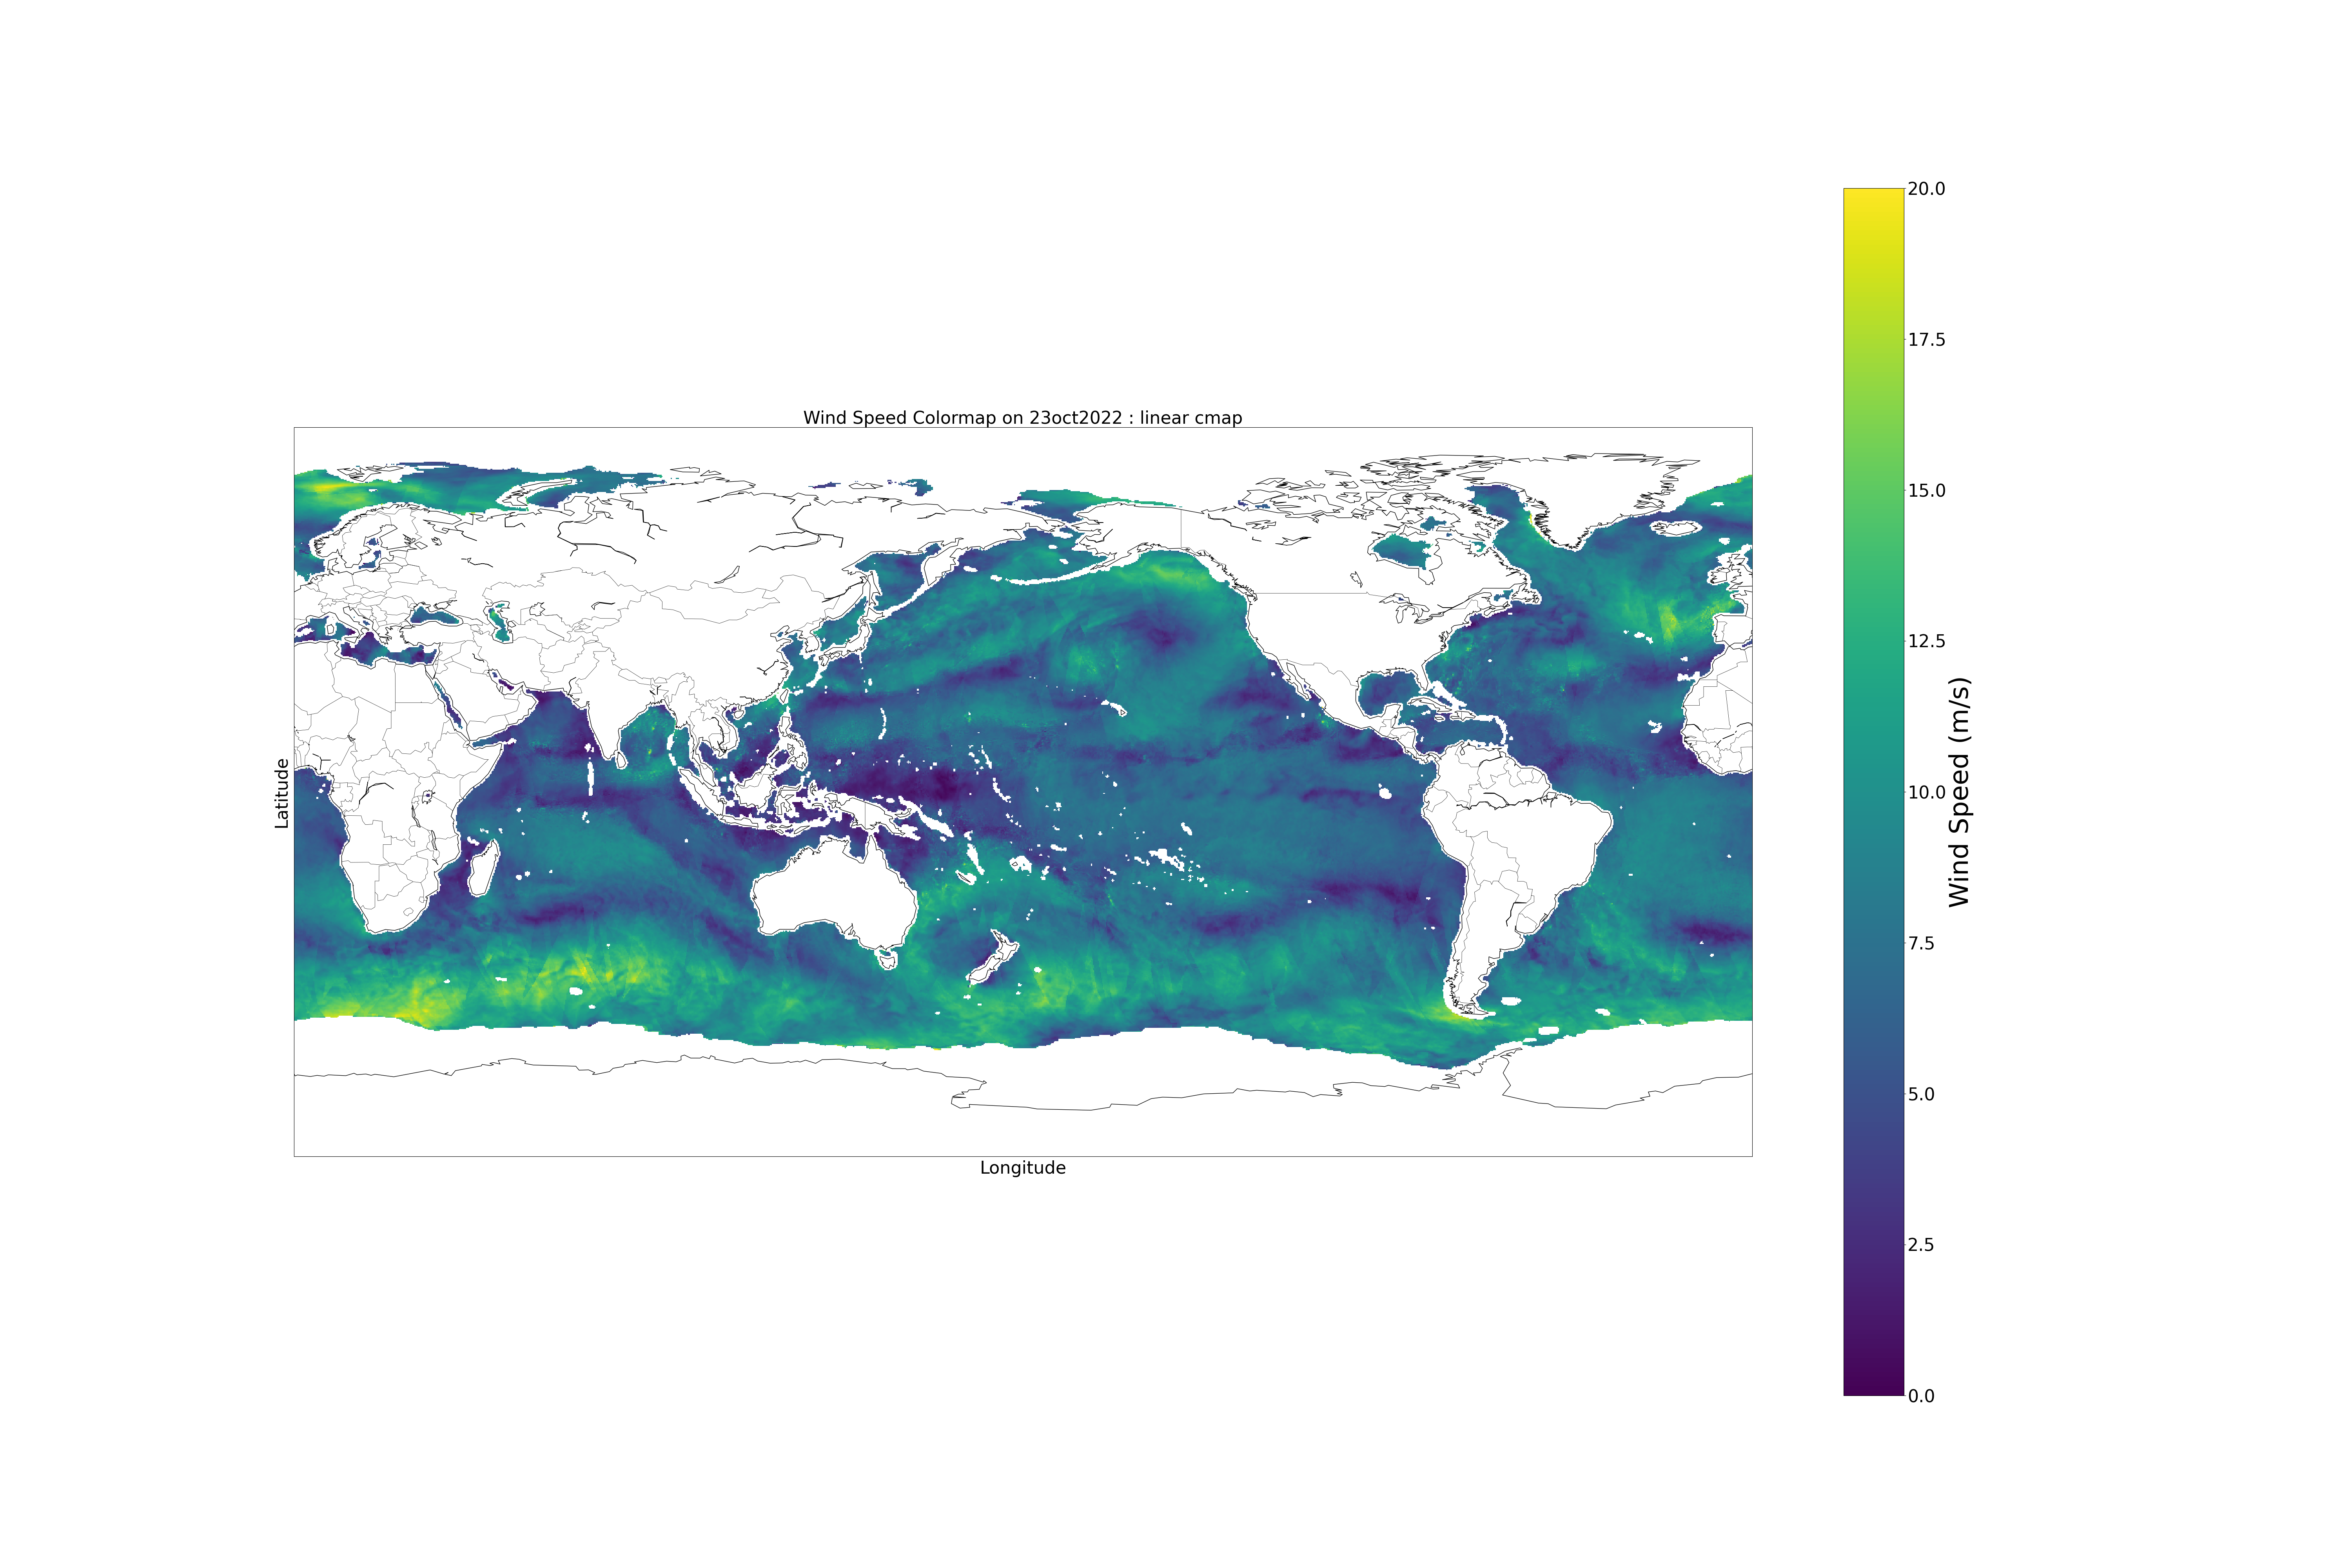
\includegraphics[scale=0.05]{images_deep/viridis_lin_23oct2022.png}
    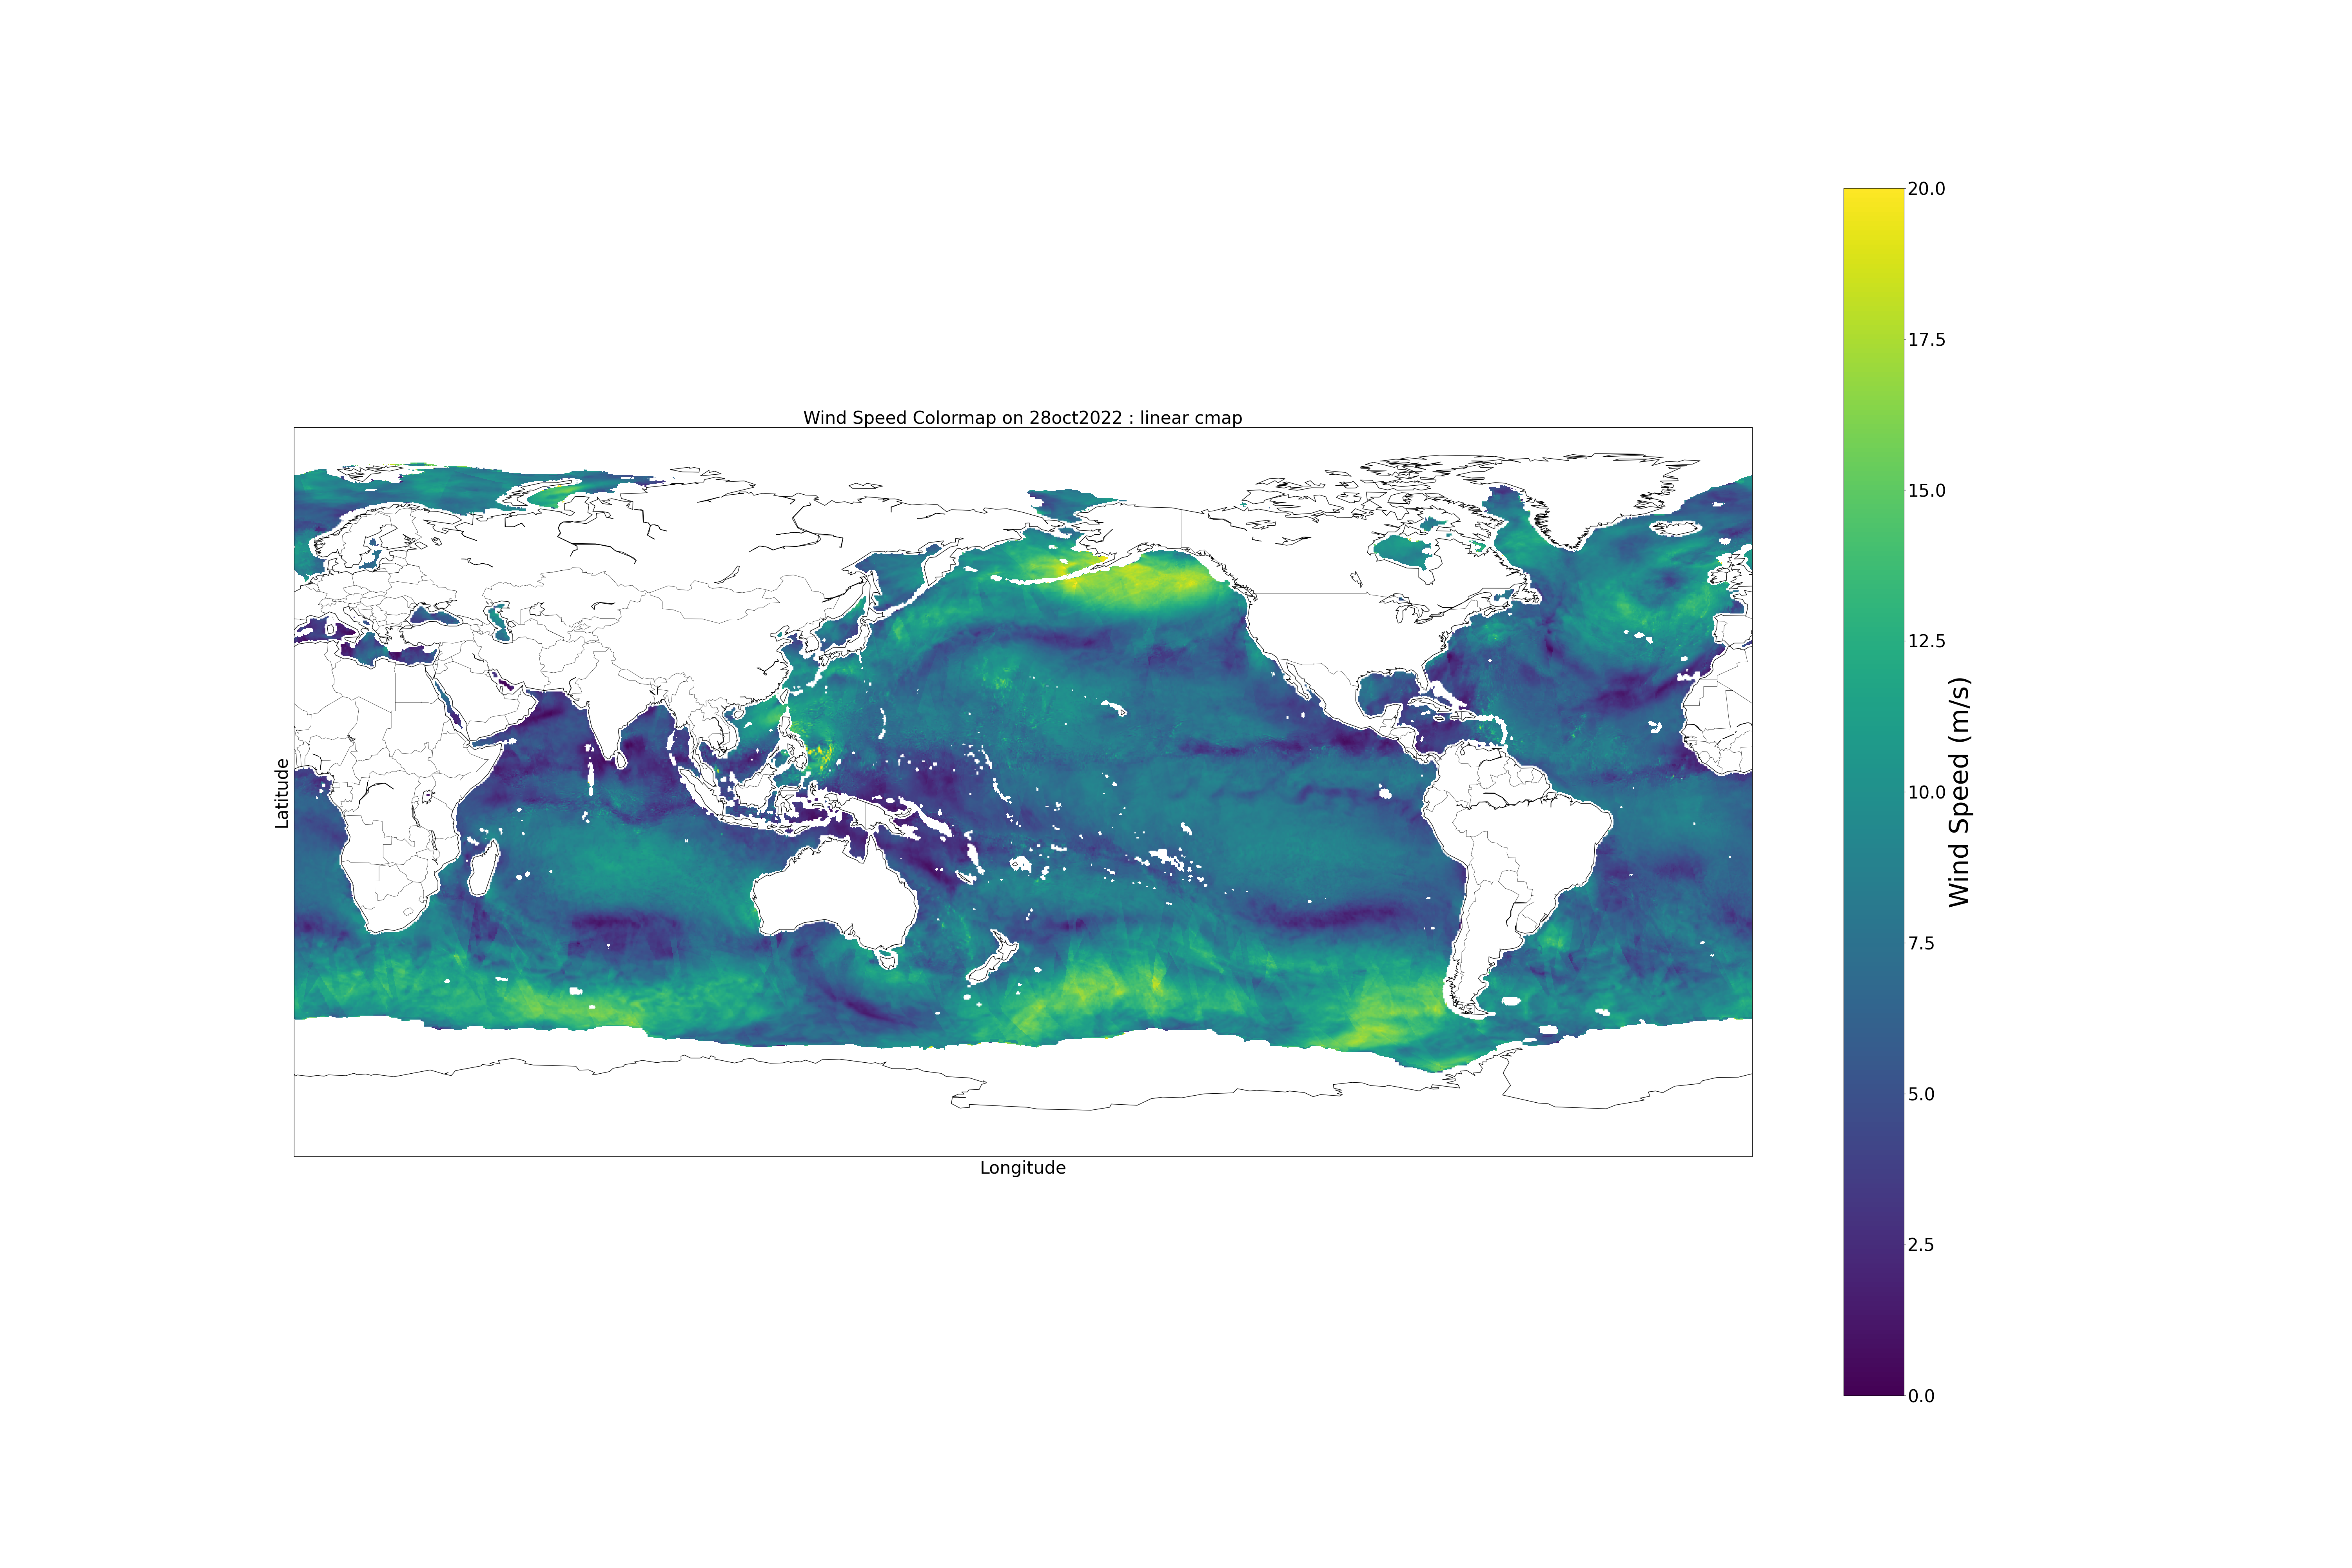
\includegraphics[scale=0.05]{images_deep/viridis_lin_28oct2022.png}
    \caption{The images correspond to the Colormap on 19, 23, and 28 October 2022 respectively, One can notice the increase of windspeed in the Bay of Bengal on 23 October 2023, caused by Cyclone Sitrang}
    \label{sitrang}
\end{figure}

\section{Contour Mapping}

Contour mapping, also known as contour plotting or contour lines, is a way to visualize data by representing constant values or isolines. Contour lines are lines that connect points with the same data value, creating curves that provide insights into the data's spatial distribution.

\subsection{Contour Lines and Contour Fill}
% The library we used in python allows use to plot contours and 
Marching Squares is an algorithm for contour mapping in 2D scalar fields. It divides a grid into cells, assigns unique codes based on corner values, and uses a lookup table to determine contour segments. By connecting these segments, it generates accurate contour lines. Contour fill, often paired with Marching Squares, involves shading the regions between contours to represent scalar variations. 


% Both the Lines and Fills are good for inference but visualizing with fills is quite easier than lines. We suggest to use colormaps instead of contour maps unless you have some peculiar thing which can be done with a contour map and not with a colormap.
Both lines and fills serve well for inference, but visualization with fills is considerably easier than with lines. We recommend opting for colormaps over contour maps unless there is a specific and unique requirement that can only be addressed with a contour map rather than a colormap.

The Python library we utilized enables us to perform both tasks. After experimenting with both approaches, we observed that the contour fill algorithm resembles using discrete color maps during color mapping. Instead of uniformly dividing the scale, you have the flexibility to divide it in the manner that suits your preferences.

As mentioned earlier, our data predominantly falls within the range of 0-20. Therefore, we created contour lines specifically for values of 8, 11, 14, and 17. We tried various colourmaps like before and as seen before we used the linear distribution and not the logrithmic distribution. We tried out  a range of diverse color maps, specifically including viridis, magma, jet, coolwarm, greys, and twilight. Among these, viridis, magma, and greys are classified as sequential color maps, while coolwarm, jet, and twilight fall under the diverging category. In this case we prefer Sequential Colourmaps over Diverging as in this case we need to refer to lines and not regions. Viridis is one we prefer.
\begin{figure}
    \centering
    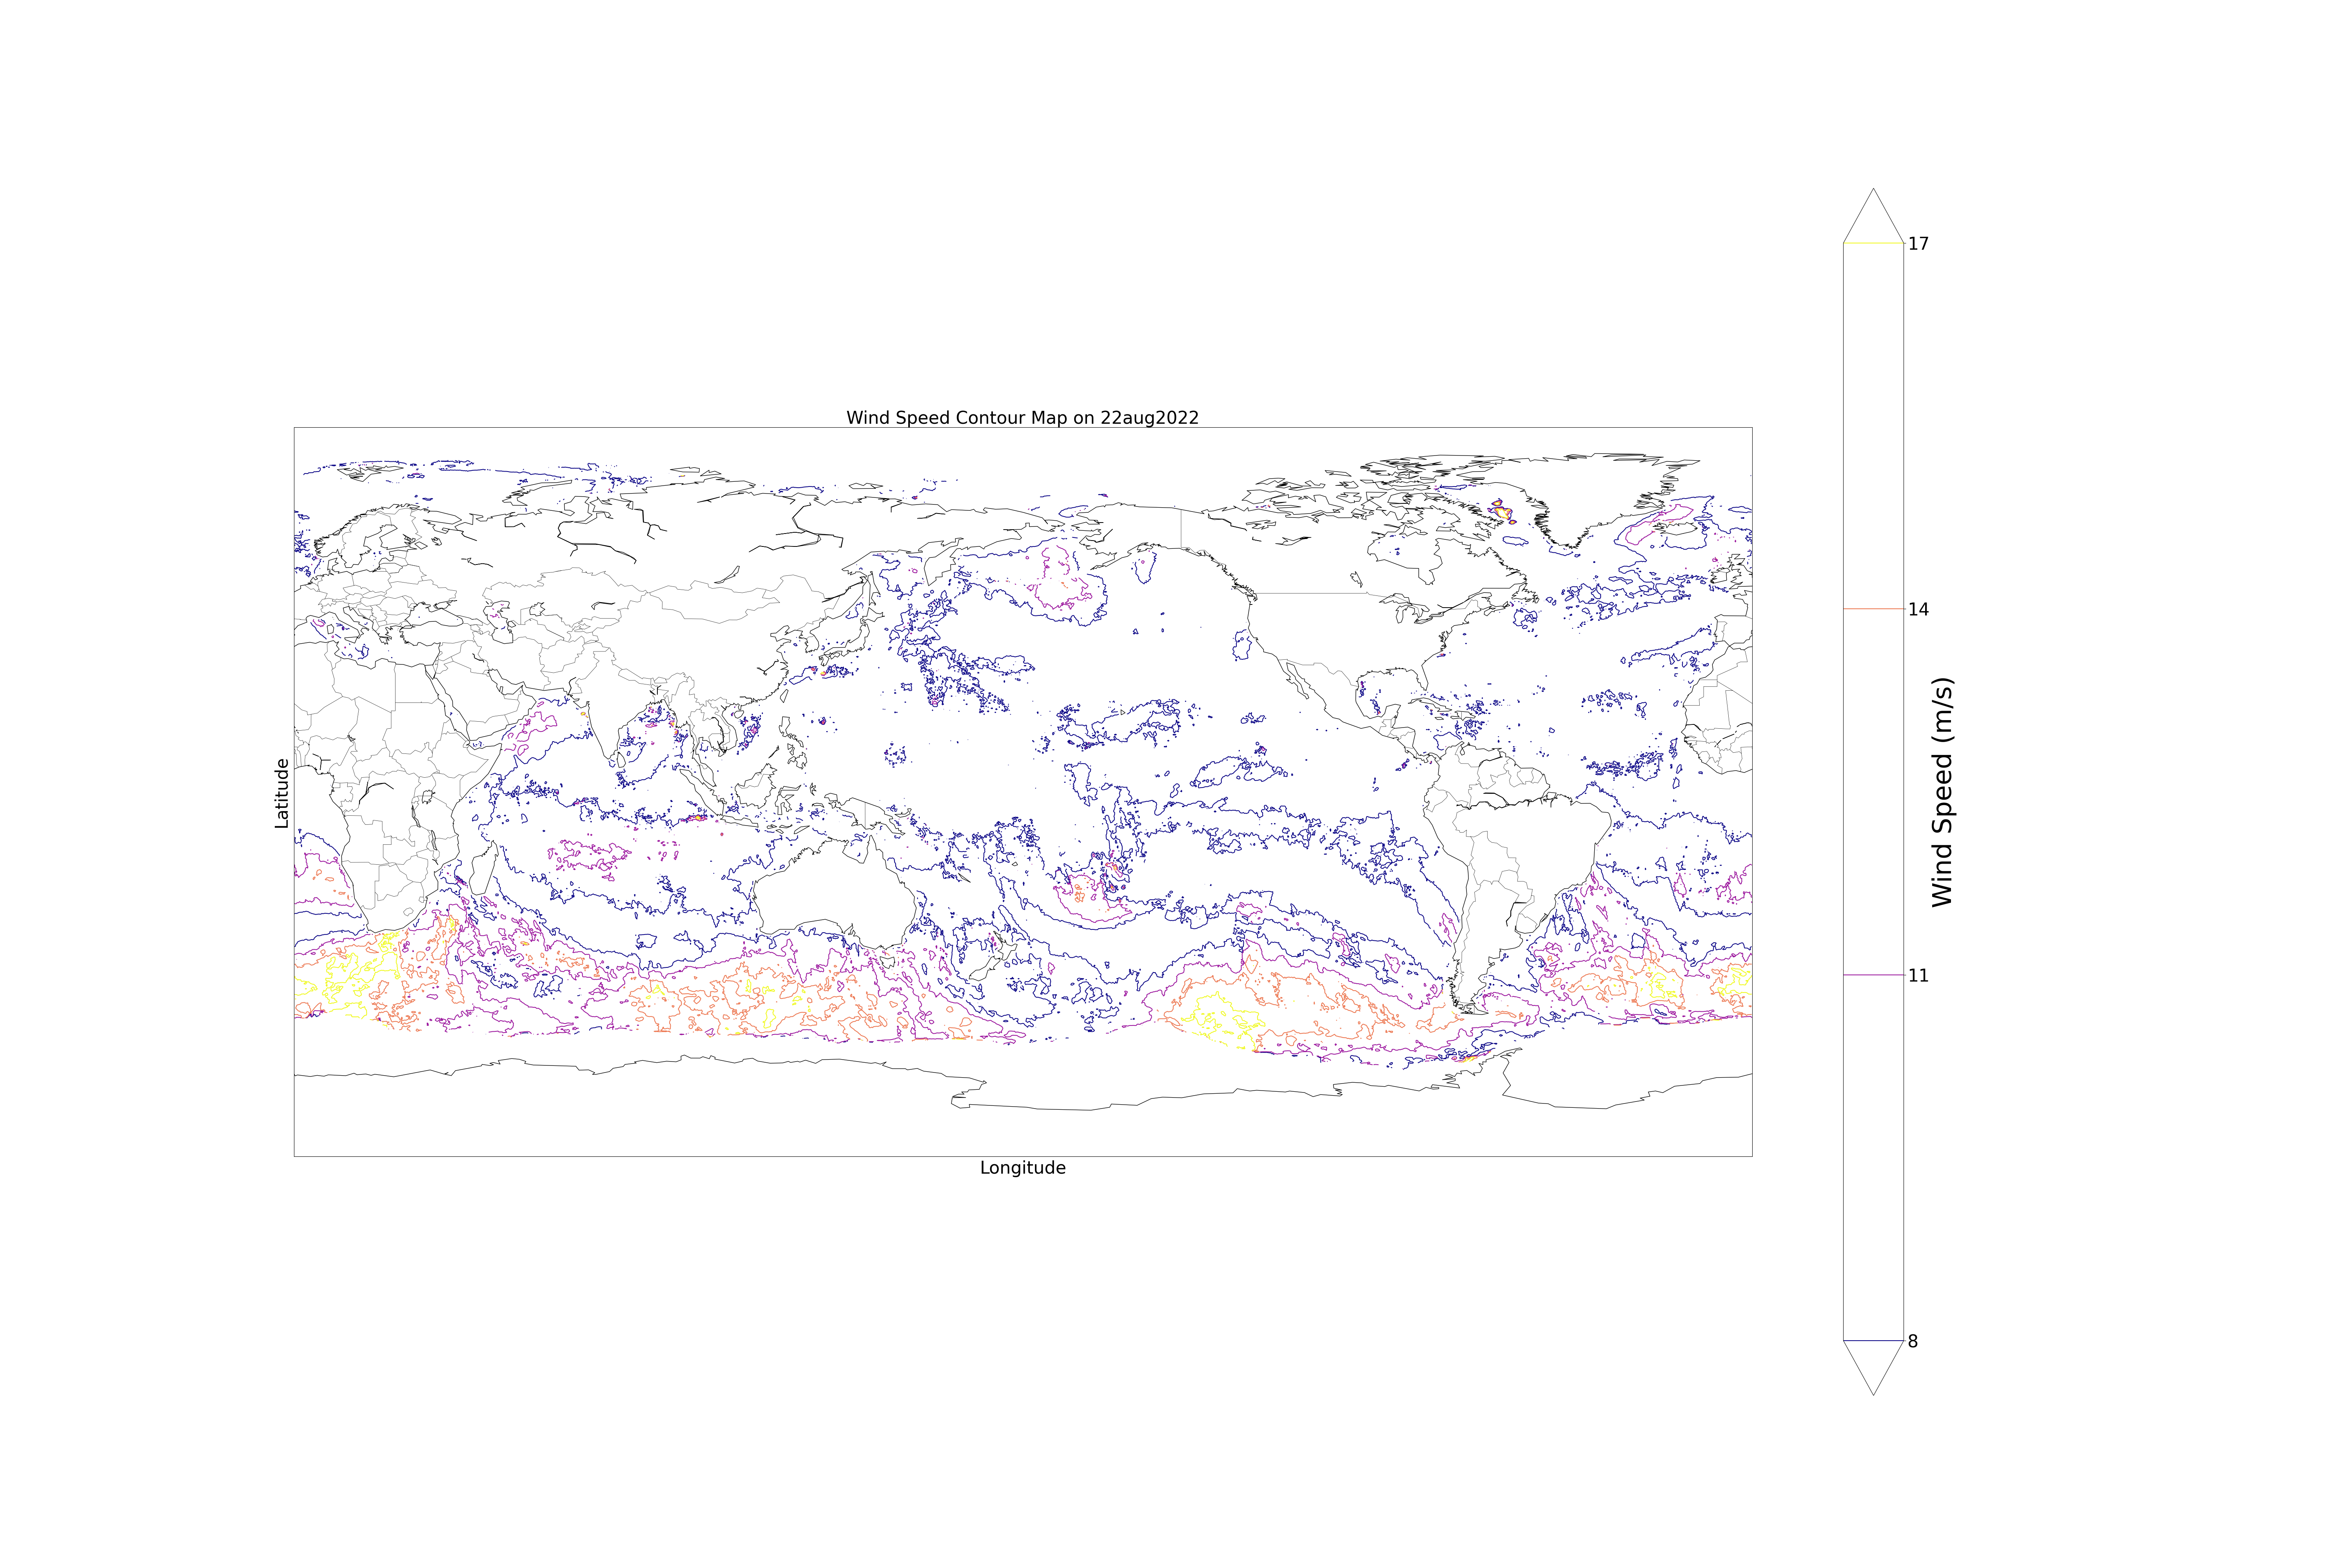
\includegraphics[scale=0.05]{images_deep/contour_plasma.png}
    \caption{contour plot from 22 August 2022}
    \label{contour}
\end{figure}


\subsection{Observations}

\begin{enumerate}

    % \item In general the concentration of he contours is more away from the equator. this suggests that the windspeed was more smooth near the equator and more uneven near the poles.
    
    % \item Lines corresponding to higher values are found near the south pole which is consistent with the findings of the colormap
    % \item Lines corresponding to higher values start cominp up in the northern part of Atlantic Ocean near the October end.
    % \item The distribution of lines along the time axis is coherent with the observations of colormap, like we see the lines corresponding to the values 14 are found more dense in the areas where the coormap showed a rise in wind speed.
    
    \item Generally, the concentration of contours is greater away from the equator. This implies that the windspeed was smoother near the equator and more erratic near the poles.

    \item Lines representing higher values are predominantly situated near the south pole, aligning with the colormap findings.
    
    \item Lines associated with higher values begin to emerge in the northern part of the Atlantic Ocean towards the end of October.
    
    \item The distribution of lines along the time axis aligns coherently with the colormap observations. For instance, areas where the colormap indicated an increase in wind speed correspondingly exhibit a denser presence of lines associated with the value 14. a range of diverse color maps, specifically including viridis, magma, jet, coolwarm, greys, and twilight. Among these, viridis, magma, and greys are classified as sequential color maps, while coolwarm, jet, and twilight fall under the diverging category.

\end{enumerate}
\begin{figure}
    \centering
    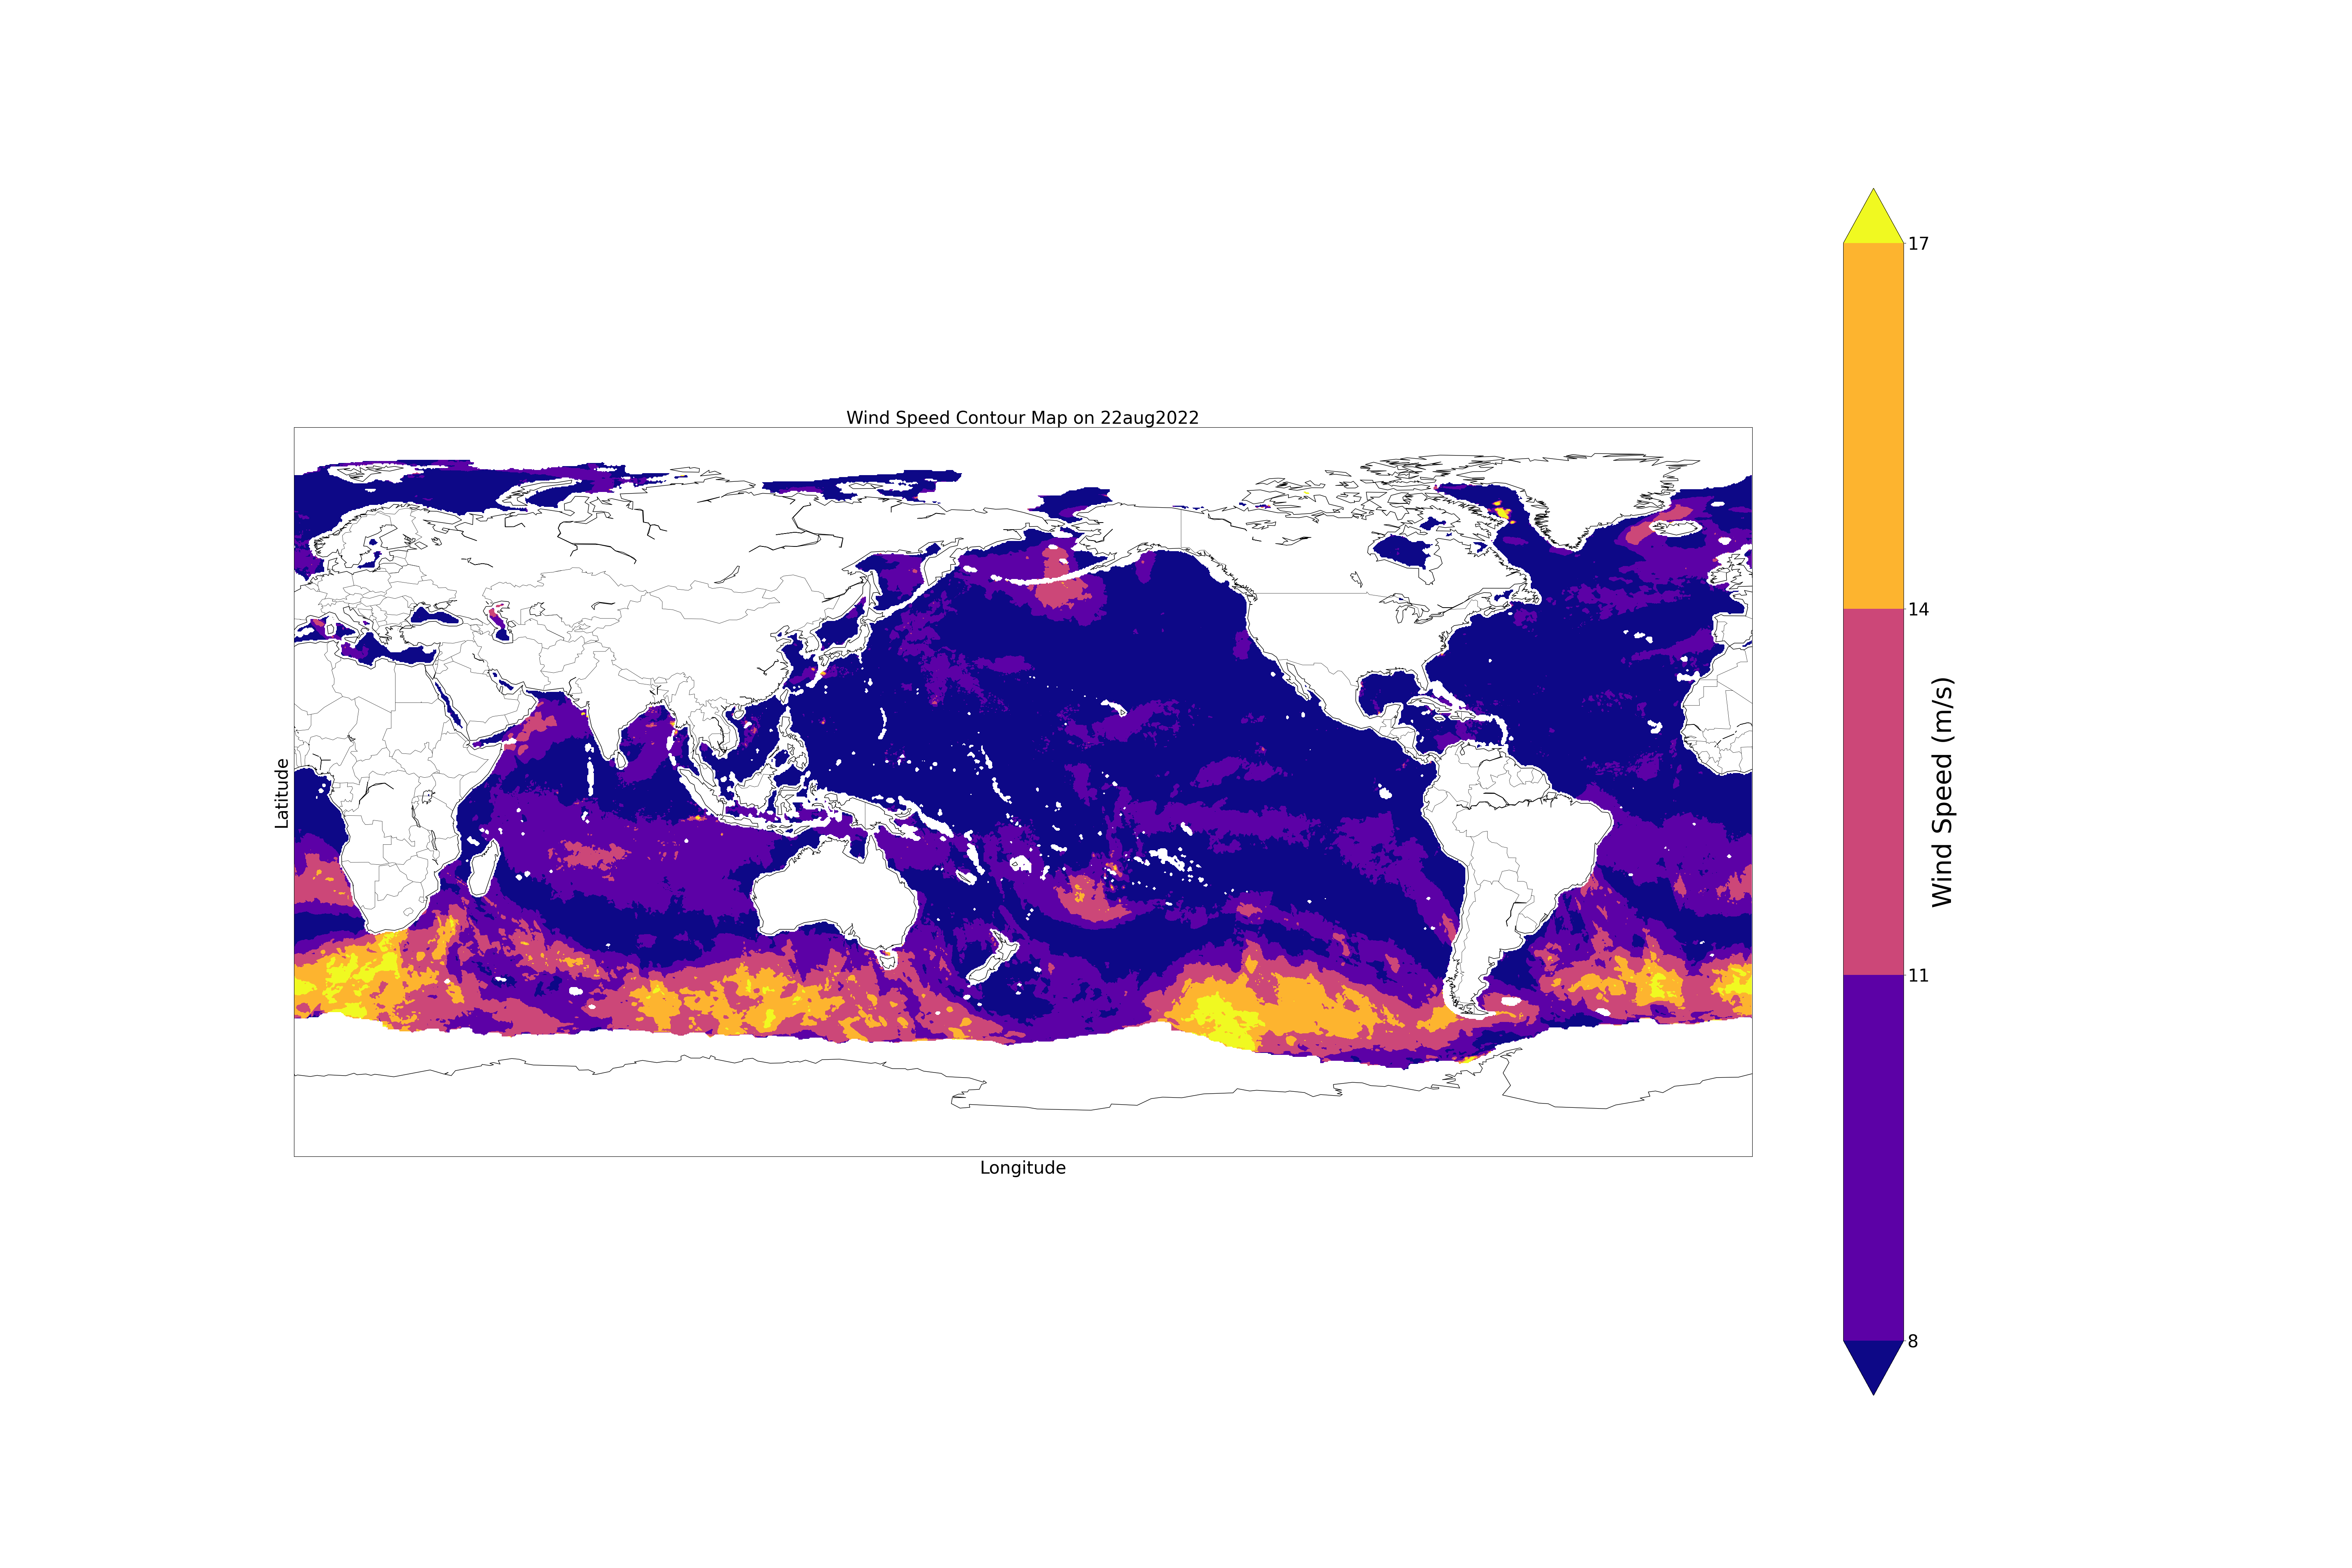
\includegraphics[scale=0.05]{images_deep/contour_plasma_fill.png}
    \caption{Contour Fill plot for 22 August 2022}
    \label{contour_fill}
\end{figure}


\section{Introduction}


\subsection{Introduction to Quiver Plots}

Quiver plots provide a visual representation of vector fields, showcasing the direction and magnitude of data points. In our context, each arrow in the quiver plot represents wind speed and direction at specific locations across the globe. This visualization method enables a rapid comprehension of global wind patterns, allowing viewers to discern both the intensity and orientation of atmospheric flows. Through quiver plots, intricate details of wind dynamics become accessible, enhancing the interpretability of meteorological data.
 

\subsection{Objective}

Our primary aim is to optimize quiver plots for visualizing and extracting insights from wind speed datasets. To achieve this, we are conducting experiments on two crucial aspects:

\begin{enumerate}
  \item \textbf{Grid Sampling:} We tried different levels of grid sampling. This was done to try to increase the redability and thus improving the inference qualities.

  \item \textbf{Vector Representations:} We also experimented with different vector representations i.e, same sized vectors or vectors with size proportional to magnutide of the wind speed at that point.
\end{enumerate}




\section{GIF Creation}

To provide a dynamic representation of the quiver plots over time, a GIF animation was generated using the \texttt{imageio} library and the stores quiver plot images.




\section{Experimentation}

\subsection{Grid sampling:} As part of grid sampling the longitudes and latitudes after every stride value were taken. The stride was set as a variable which was changed as part of experimentation. This reduces or increases the density of vectors in the plot which changes the redability and inference qualities. 

\subsection{Vector magnitude:} For this in the first part the length of vectors were kept same for the while plot and only the length was changed to increase redability. In the second part the length of the vectors were kept proportional to wind speed at that point scaled by a constant value which could be changed for experimentation.



\section{Results}

\subsection{Grid Sampling Analysis}

To evaluate the impact of grid sampling on the clarity and informativeness of quiver plots, three representative plots were generated with varying strides. The following observations were made:

\begin{itemize}
  \item \textbf{Very Low Stride (Too Many Arrows):} The quiver plot with only 2 stride resulted in an excessive number of arrows, making it challenging to discern meaningful patterns due to overcrowding. This is illustrated in Figure \ref{fig:no_stride}.

  \begin{figure}[h]
    \centering
    \includegraphics[width=0.7\linewidth]{images_ricky/quiver_plot_stride_2.png}
    \caption{Quiver Plot with Stride 2}
    \label{fig:no_stride}
  \end{figure}

  \item \textbf{Normal Stride:} A quiver plot with a moderate stride provided a balanced representation of wind patterns, offering sufficient granularity for interpretation without overwhelming the visualization. This is exemplified in Figure \ref{fig:normal_stride}.

  \begin{figure}[h]
    \centering
    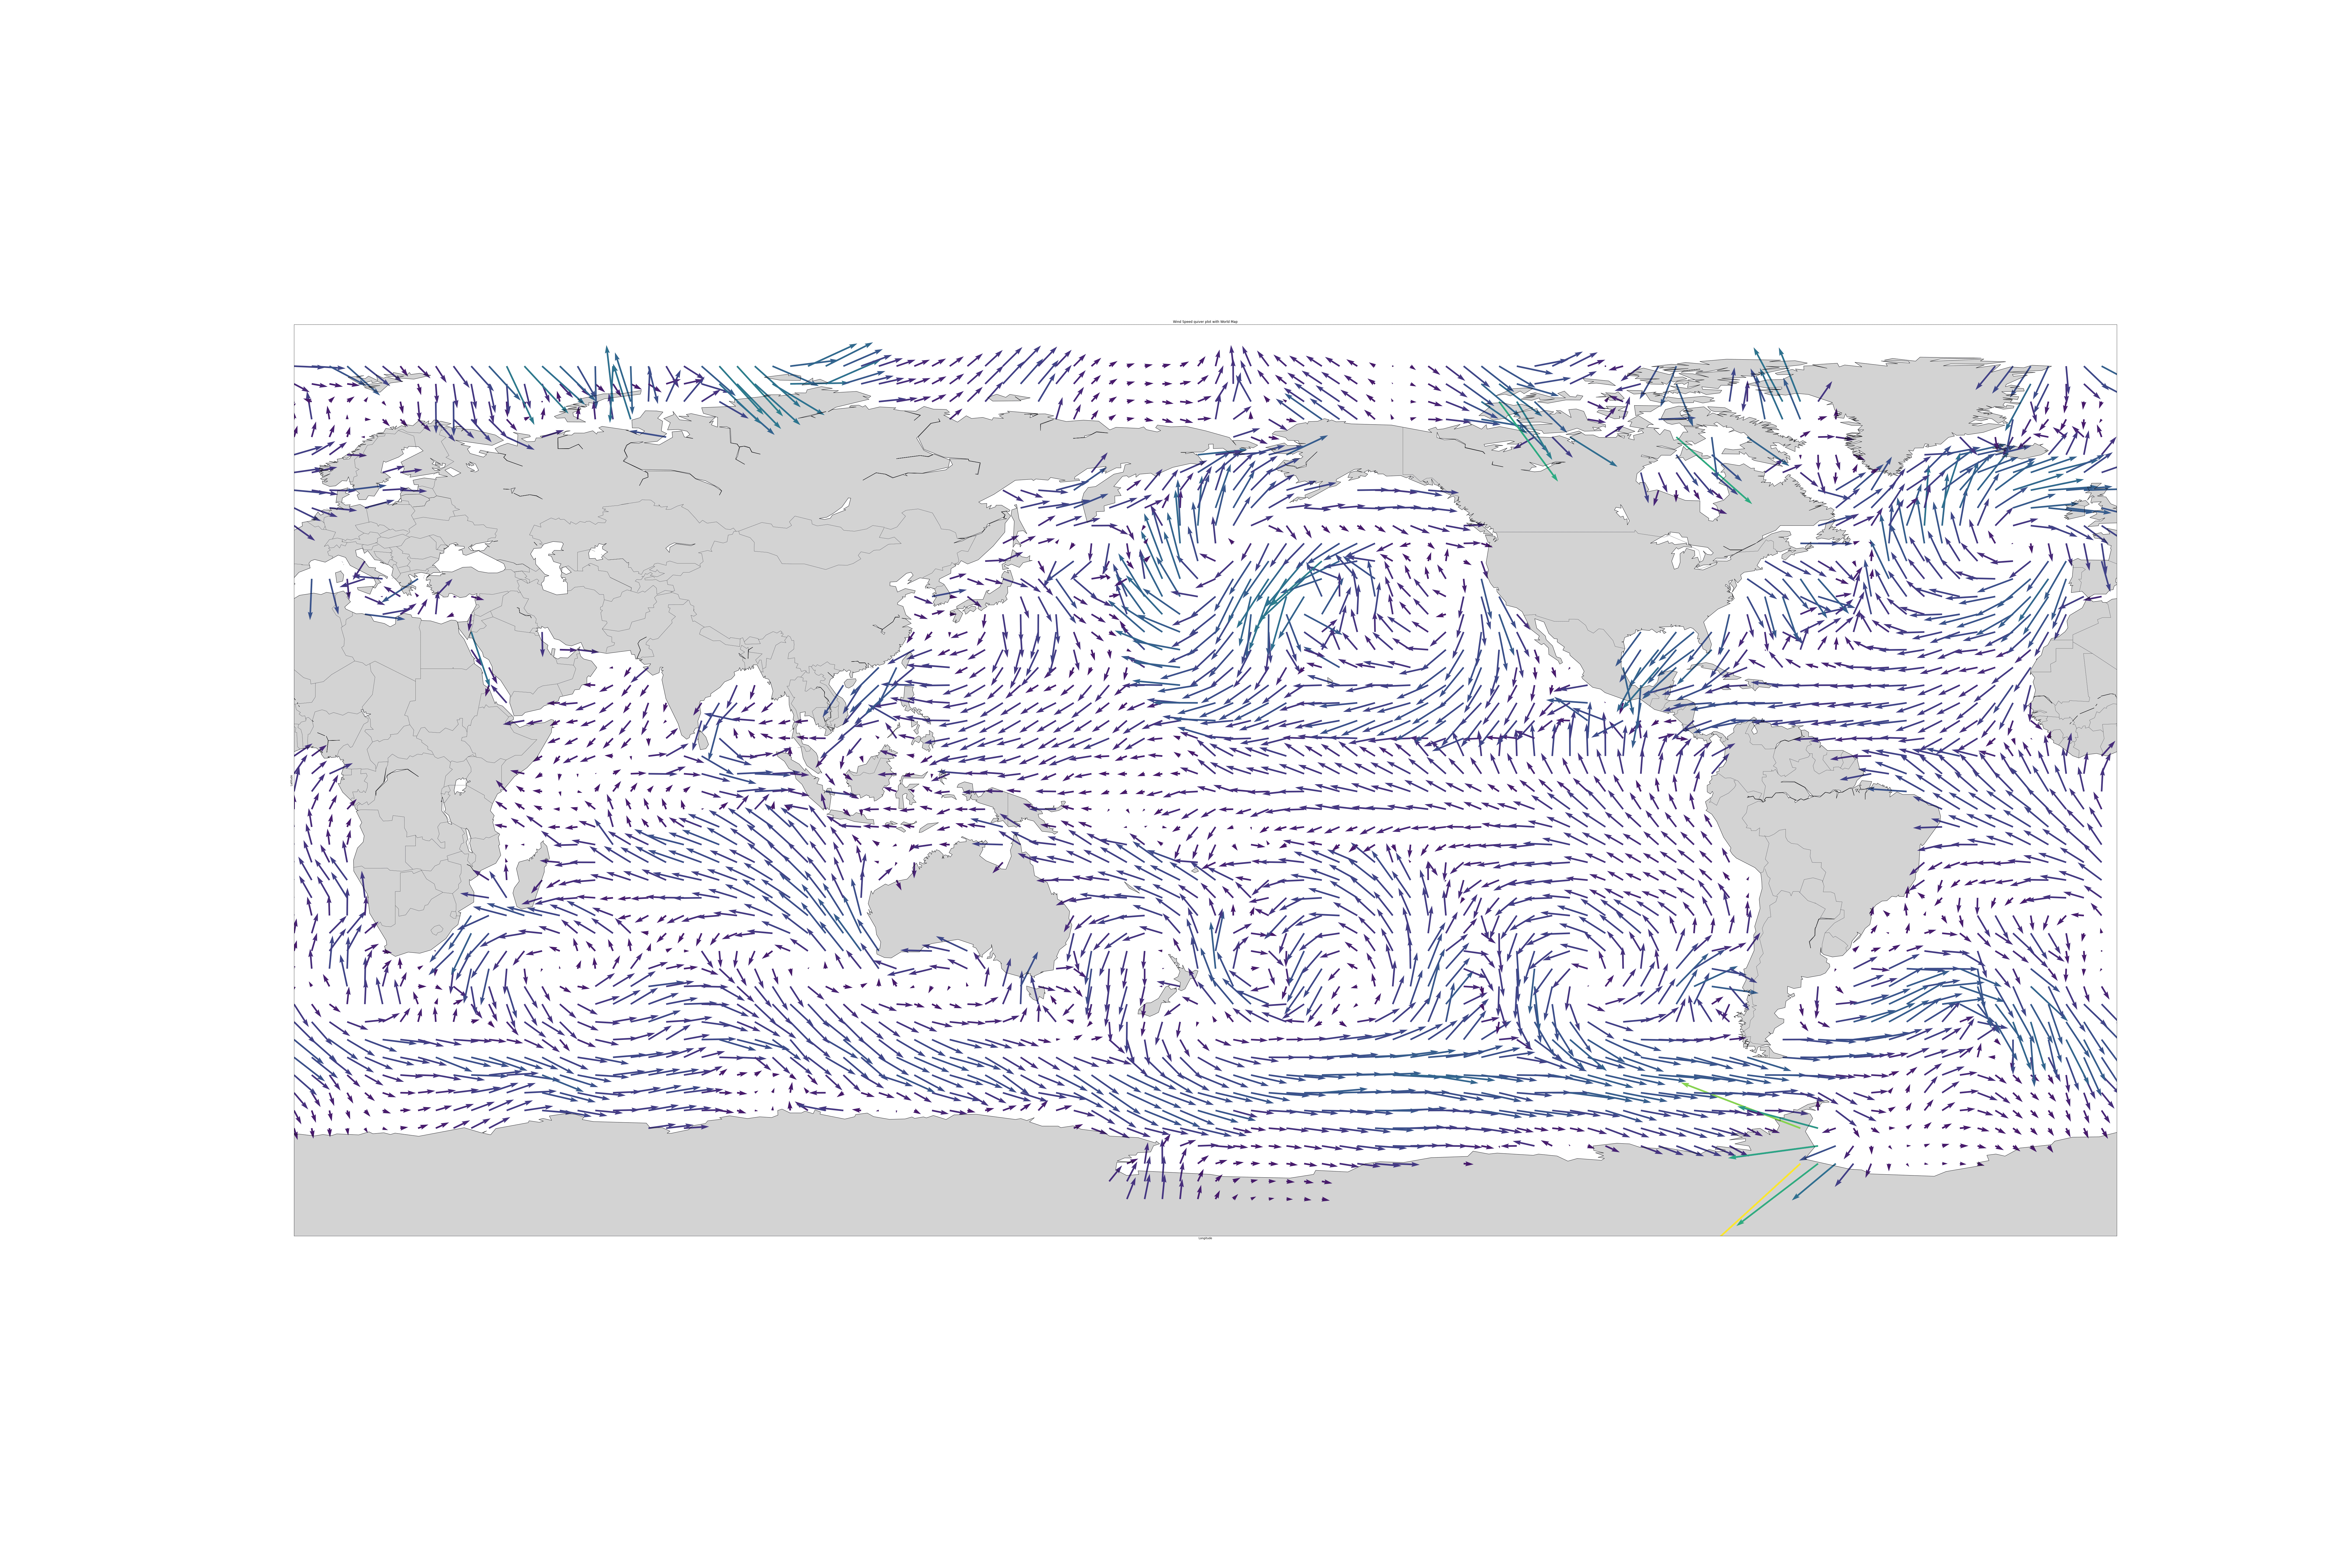
\includegraphics[width=0.7\linewidth]{images_ricky/quiver_plot_stride_7.png}
    \caption{Quiver Plot with Normal Stride}
    \label{fig:normal_stride}
  \end{figure}

  \item \textbf{Too Much Stride:} Conversely, using a high stride resulted in a sparse distribution of arrows, potentially missing finer details in the wind speed variations. This is demonstrated in Figure \ref{fig:too_much_stride}.

  \begin{figure}[h]
    \centering
    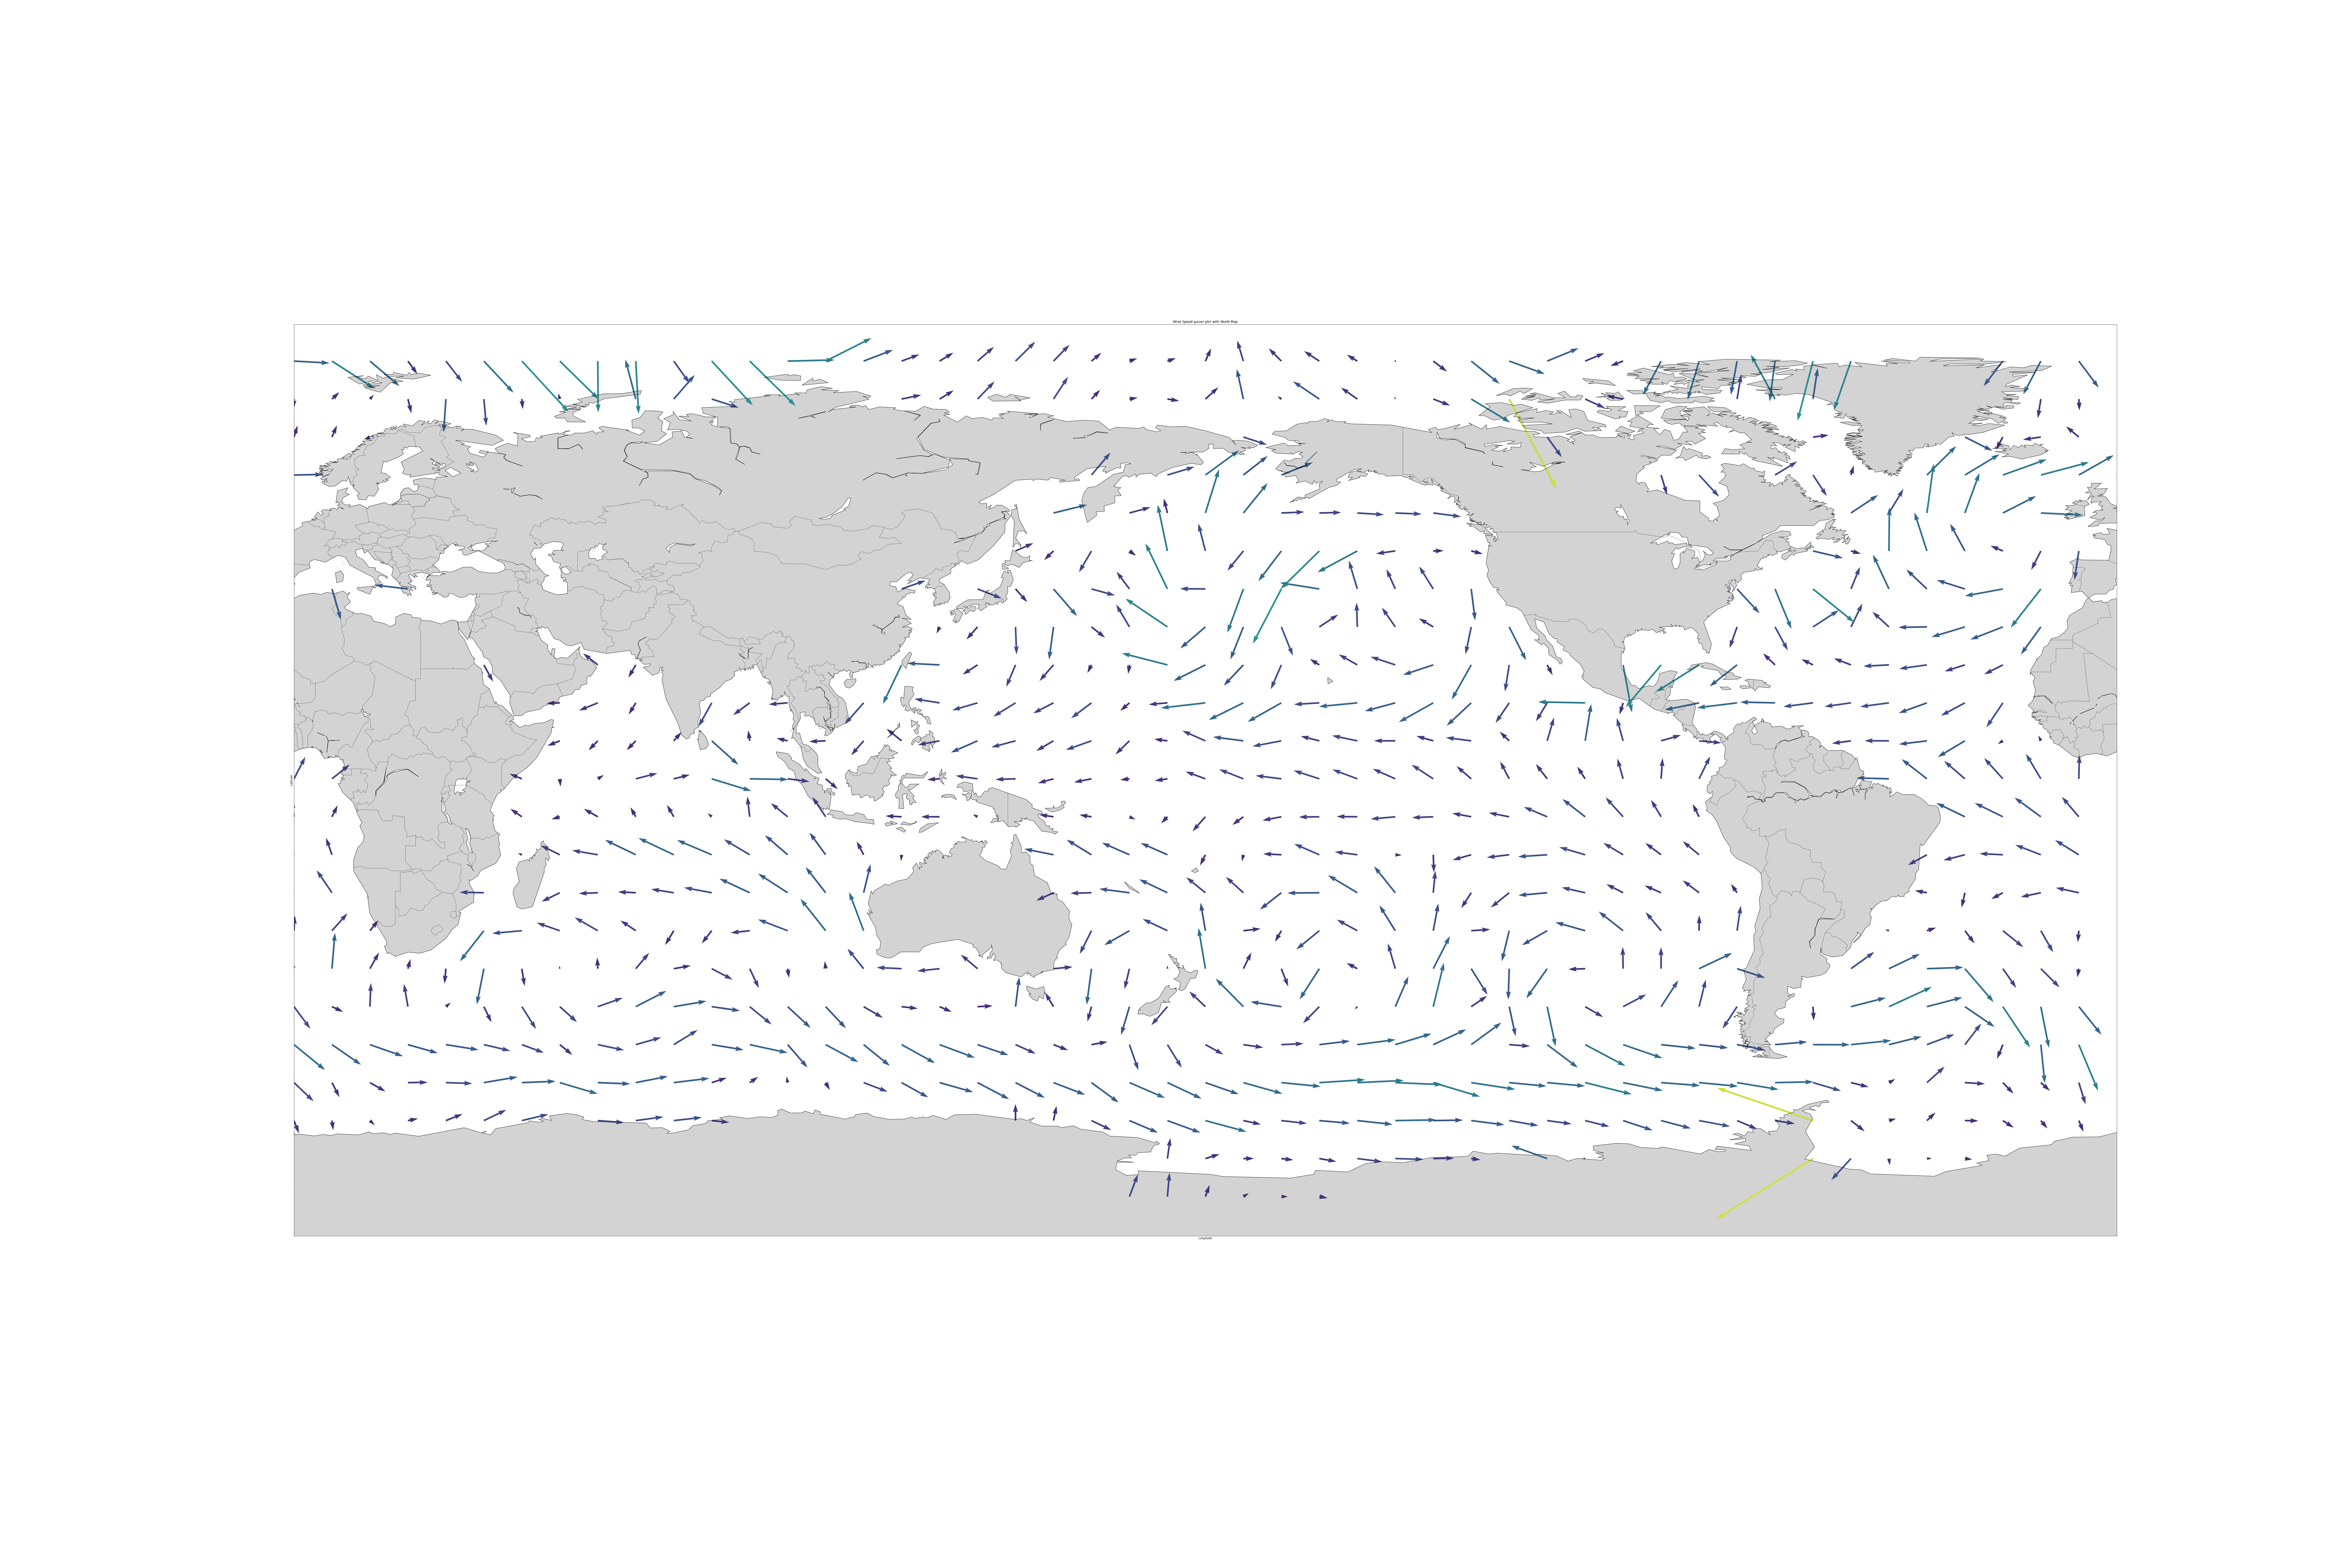
\includegraphics[width=0.7\linewidth]{images_ricky/quiver_plot_stride_15.png}
    \caption{Quiver Plot with Too Much Stride}
    \label{fig:too_much_stride}
  \end{figure}

\end{itemize}

\subsection{Comparison of Vector Representations}

To assess the impact of vector representations on the interpretability of quiver plots, two distinct approaches were employed:

\begin{itemize}
  \item \textbf{Magnitude-Proportional Vectors:} In this representation, vectors were scaled according to their magnitudes, providing a visual emphasis on areas with higher wind speeds. Figure \ref{fig:magnitude_proportional} illustrates the quiver plot using magnitude-proportional vectors.

  \begin{figure}[h]
    \centering
    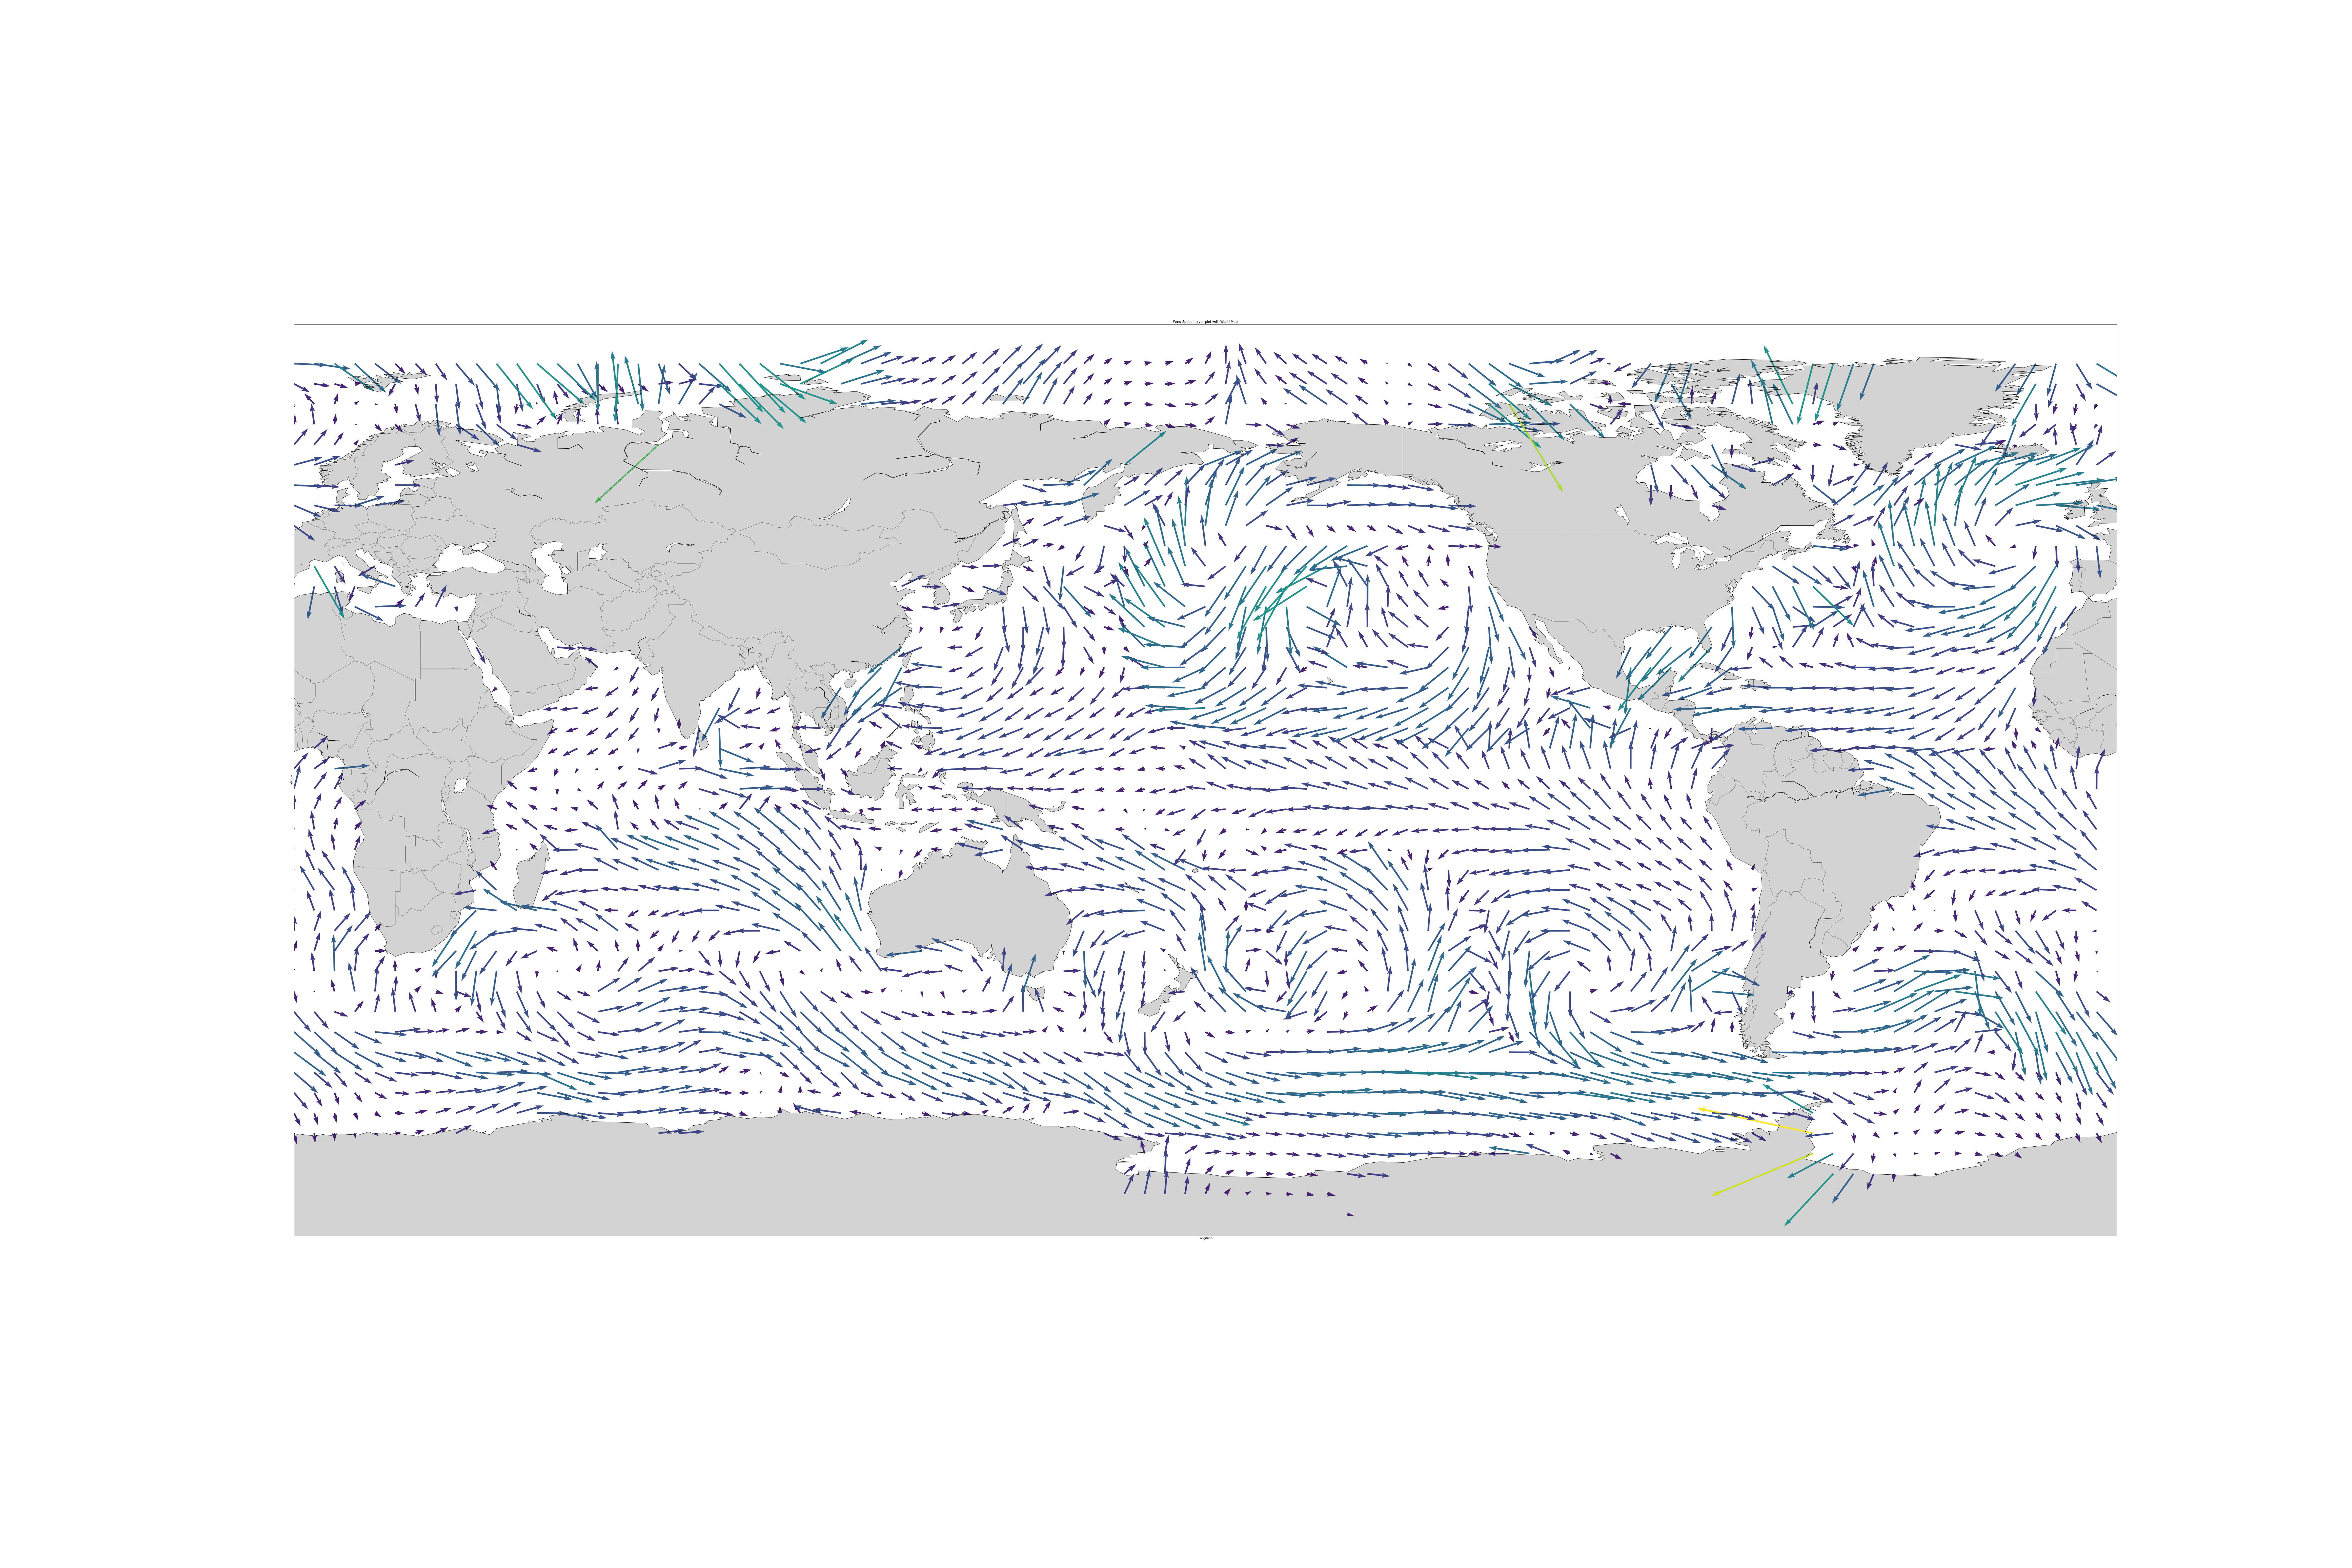
\includegraphics[width=0.7\linewidth]{images_ricky/quiver_plot_different.png}
    \caption{Quiver Plot with Magnitude-Proportional Vectors}
    \label{fig:magnitude_proportional}
  \end{figure}

  \item \textbf{Same-Sized Vectors:} Alternatively, vectors of uniform length were employed, enhancing the uniformity of the plot's visual representation. This is showcased in Figure \ref{fig:same_sized_vectors}.

  \begin{figure}[h]
    \centering
    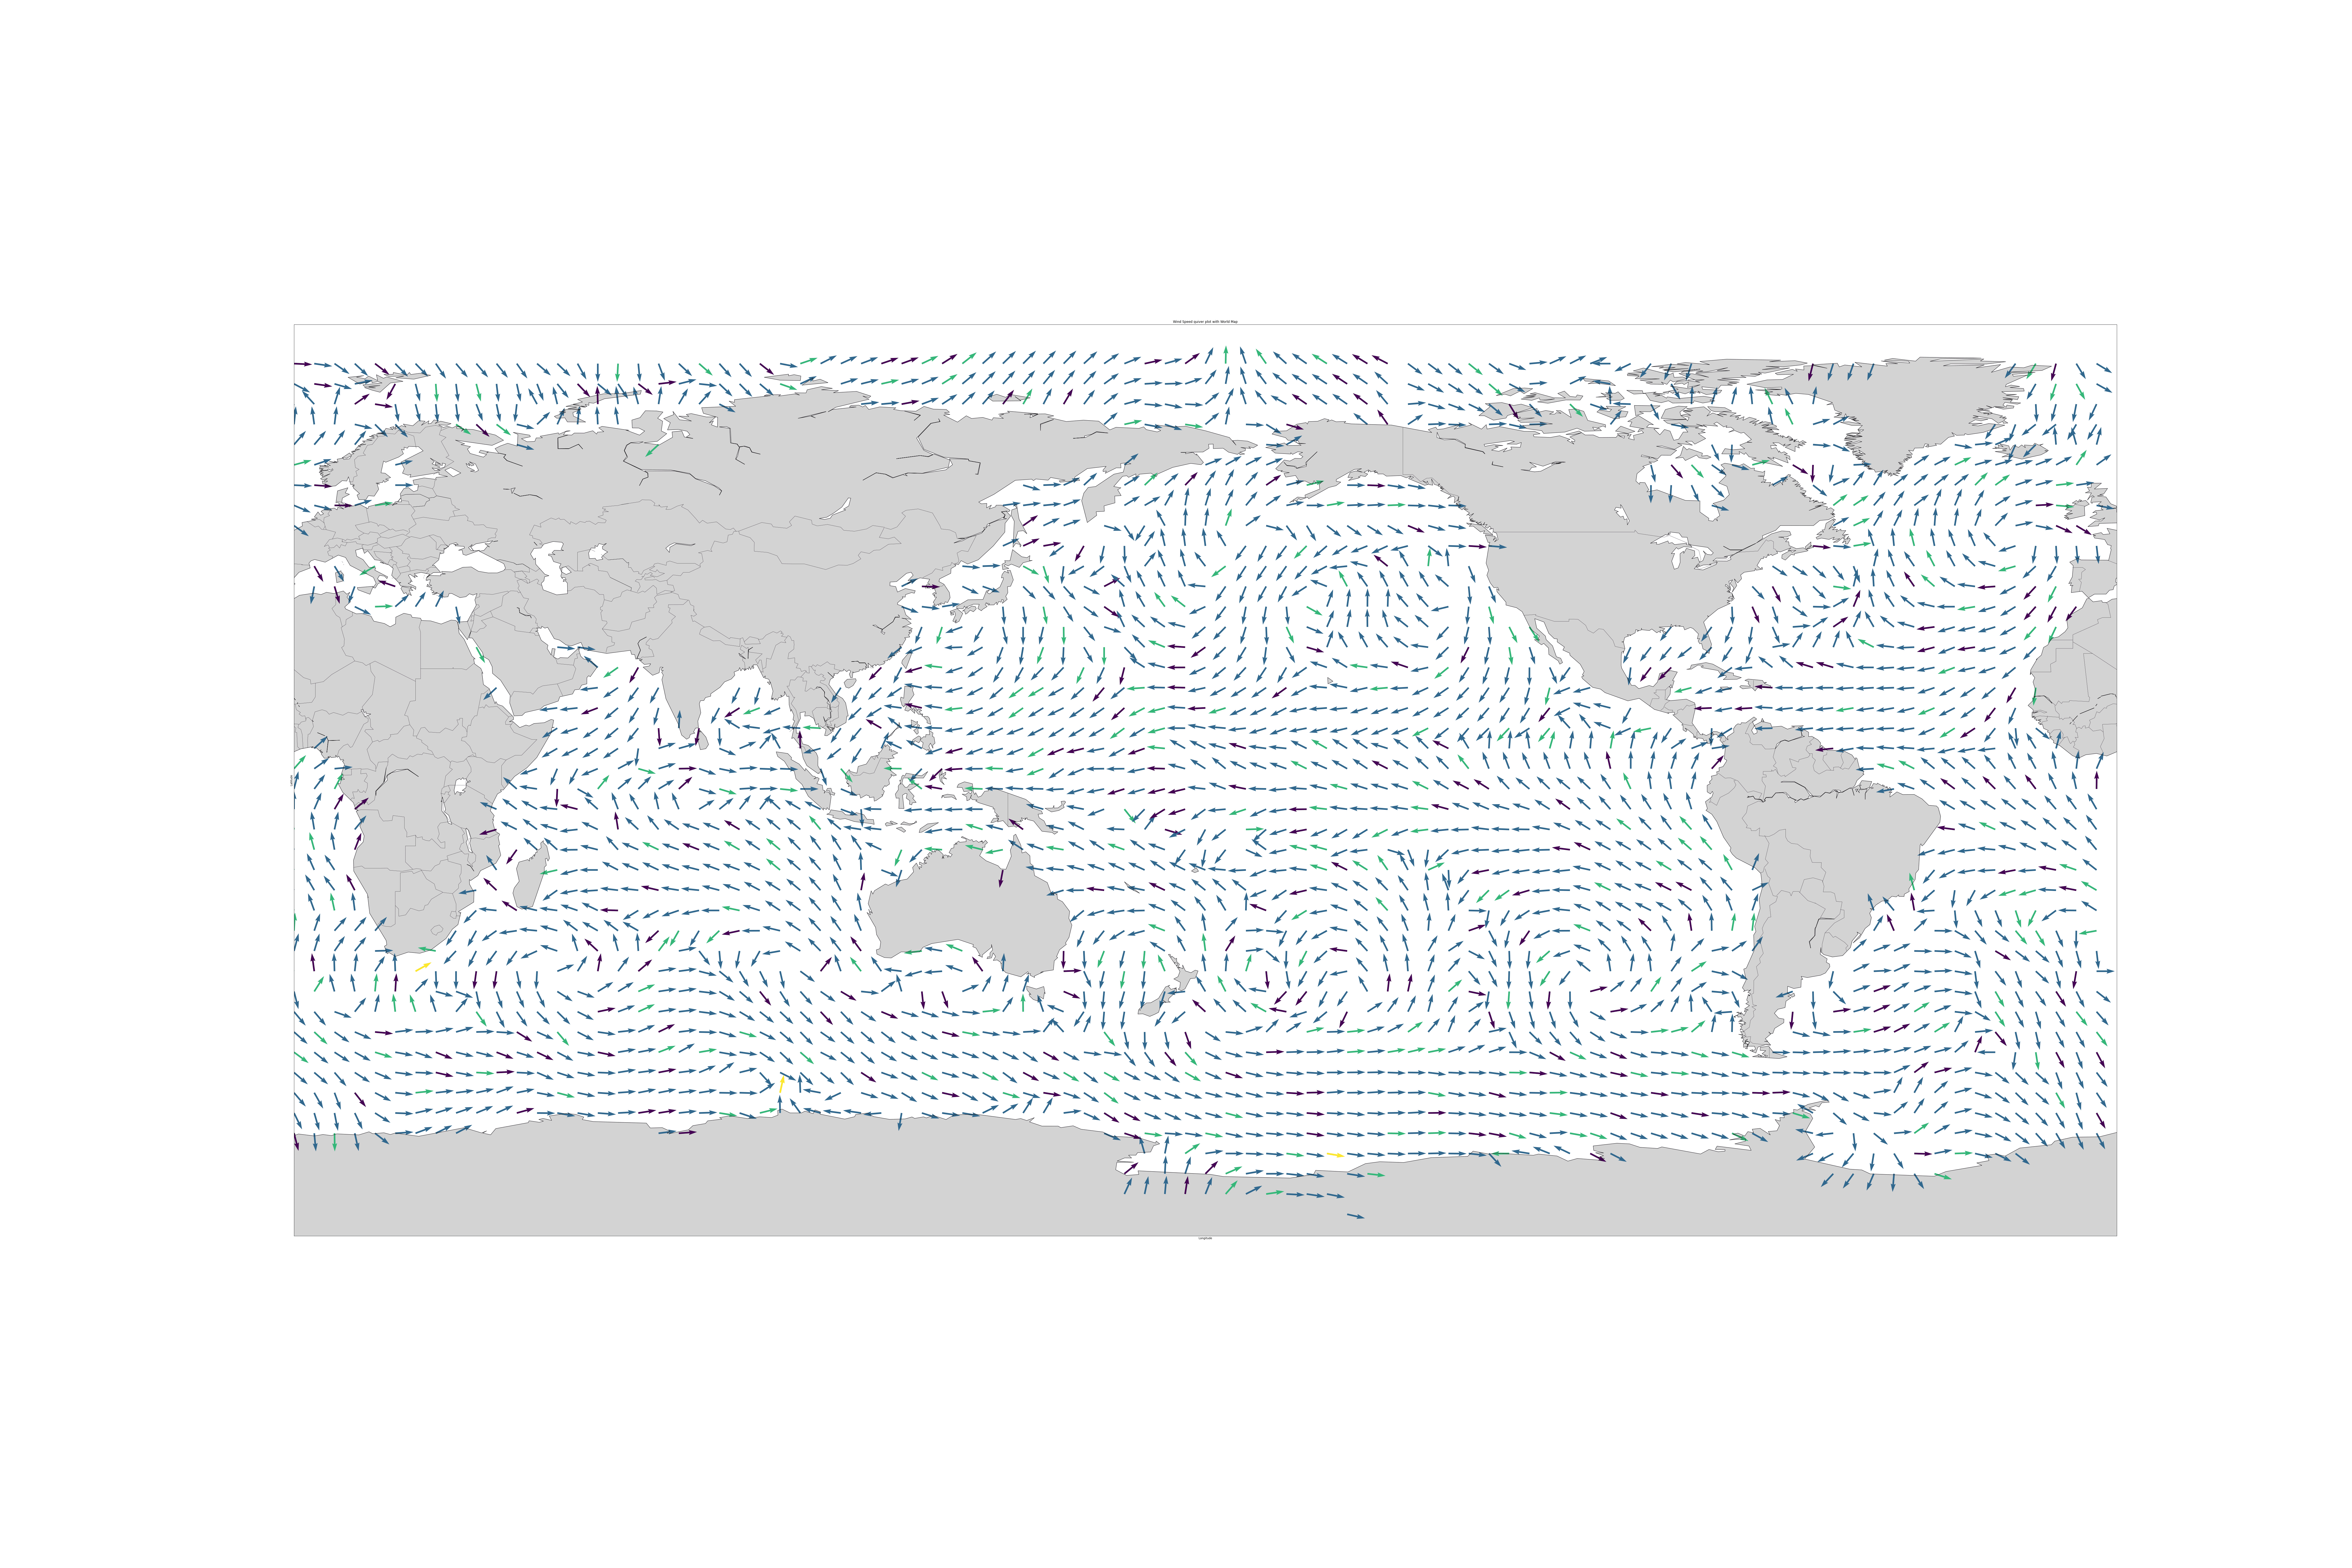
\includegraphics[width=0.7\linewidth]{images_ricky/quiver_plot_same.png}
    \caption{Quiver Plot with Same-Sized Vectors}
    \label{fig:same_sized_vectors}
  \end{figure}

\end{itemize}

The comparisons outlined above provide insights into the optimal configurations for grid sampling and vector representations in quiver plots, contributing to the creation of more readable and informative visualizations.




\section{Inferences from Quiver Plots}

\begin{itemize}
  \item Almost for the whole month of novermber 2013 the windspeed were quite high in souther pacific ocean.

  \item From 2nd-November to 14th november the windSpeed in the north atlantic region near green land kept on increasing at a rapid rate and from then on the windSpeeds started decreasing. The quivers around that point hints toward a cyclone. Infact there was the Hurricane Ingrid at that point of time around that part of the world.

  \item Overall the windspeeds were quite low in the indian-ocean during the whole november 2013.

\end{itemize}

\section{Information Visualization}
We have used the dataset which provides information about the GDP (Gross Domestic Product) of about 177 countries around the world in the year 2022.The data is taken from World Bank dataset. It has the columns:\\
GDP\_Nominal: The nominal GDP of the country in US dollars.\\
GDP\_abbrev: The nominal GDP of the country in abbreviated form (trillion or billion).\\
GDP\_growth: The GDP growth rate of the country.\\
Population: The population of the country.\\
GDP\_PerCapita: The GDP per capita, of the country.\\
Share\_of\_WorldGDP: The share of the world's GDP contributed by the country.\\
We have added a new column called Continent to the dataset. The continent to which the country belongs.\\ 
And also we have another dataset which provides economic indicators for India over a span of several years. 
 Here's a brief description of the columns in the dataset:\\
The dataset provides economic indicators for India over a span of several years. Here's a brief description of the columns in the dataset:
Year: The year of the recorded data.\\
GDP\_Nominal: Nominal Gross Domestic Product (GDP) is the total value of goods and services produced by a country, not adjusted for inflation.\\
GDP\_Real: Real Gross Domestic Product is the total value of goods and services adjusted for inflation, providing a more accurate representation of economic growth.\\
GDP\_Change: The percentage change in GDP from the previous year, indicating the economic growth or contraction.\\
GDP\_PerCapita: GDP per capita is the GDP divided by the population, representing the average economic output per person.\\
Population\_change: The percentage change in population from the previous year.\\
Population: The total population of India in a given year.\\
We have chosen these datasets because these datasets were very much related to our A1 dataset.
\subsection{Treemap}
\begin{figure*}
\centering
    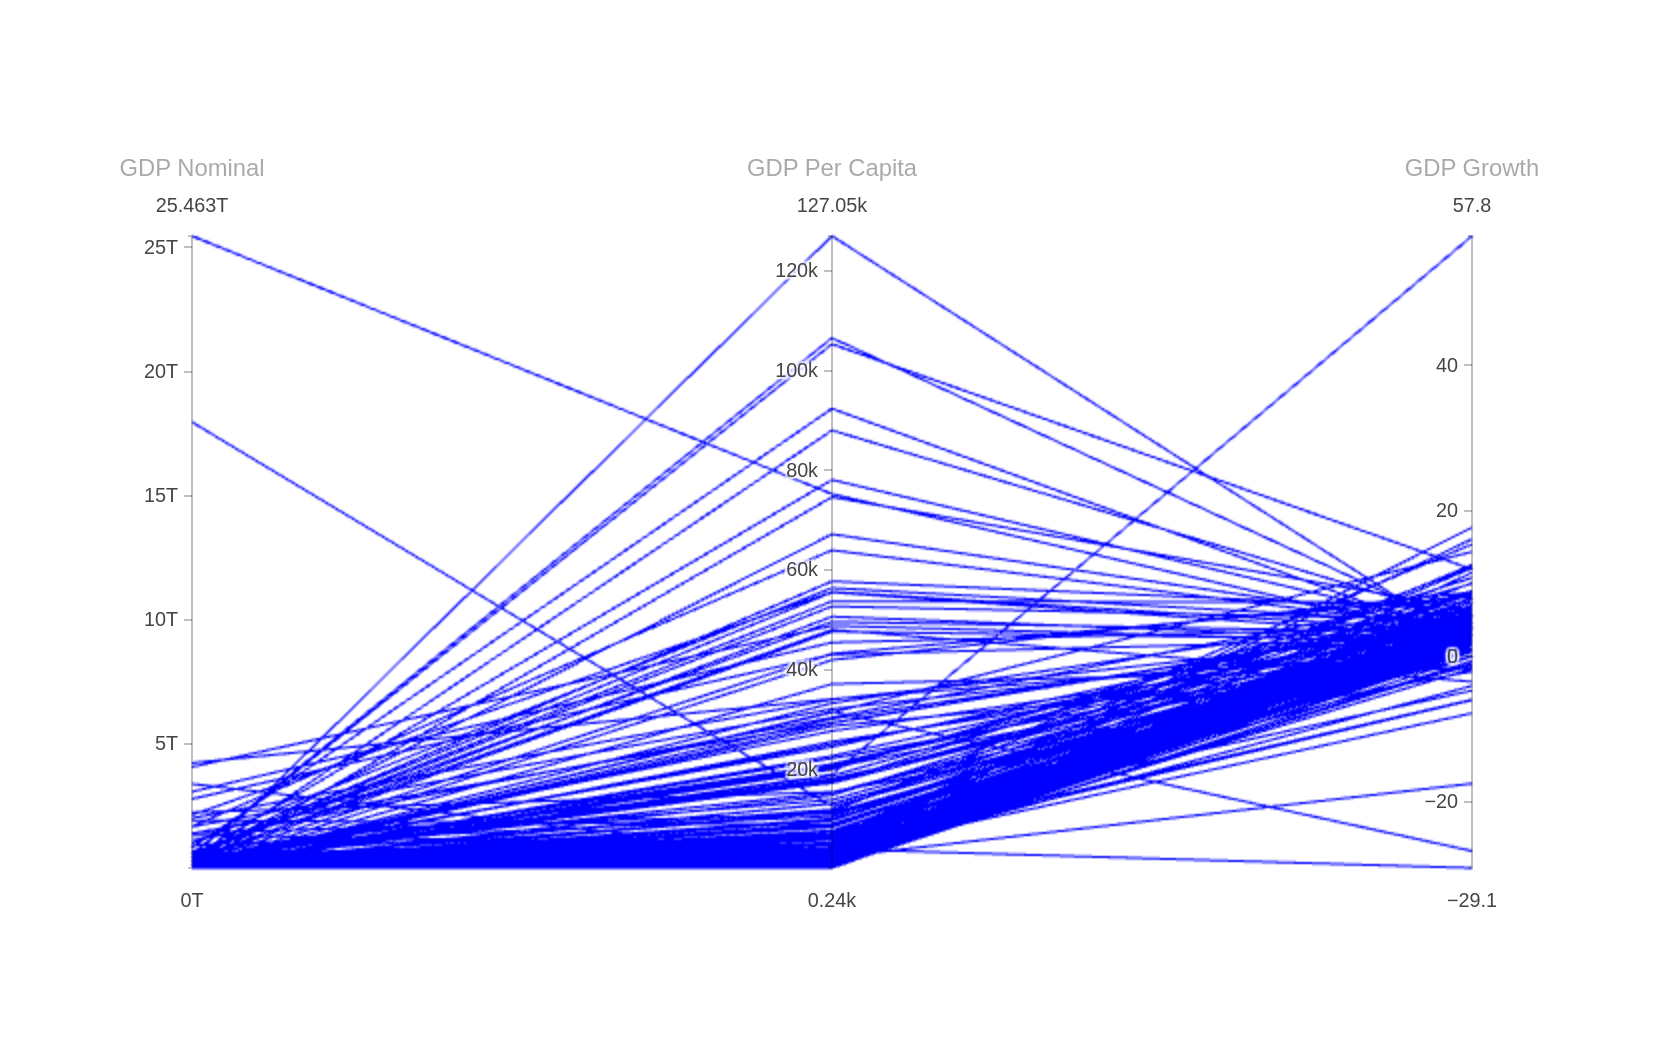
\includegraphics[height=3in, width=0.75\textwidth]{images_ashish/pcp_1.png}
    \caption{Treemap 1}
    \label{fig_1}
\end{figure*}

\textbf{Treemap - I}\\
Here is a sorted treemap (Figure \ref{fig_1} where the size of each rectangle represents the population of the country.\\
\underline{\textbf{Inferences}}\\
Population Distribution: You can observe the distribution of population sizes among countries. Larger rectangles indicate countries with higher populations, while smaller rectangles represent countries with smaller populations. You can see that China had the largest population in the year 2022.\\
Comparison of Populations: By looking at the relative sizes of the rectangles, you can quickly compare the populations of different countries. This visual representation makes it easy to identify the most populous countries and those with smaller populations.\\
Land Area vs Population: There are smaller countries with unexpectedly large populations, this was an interesting point to notice. That is even though the land area of Bangladesh is very small its population is comparable to a large country like Brazil.
\begin{figure*}
\centering
    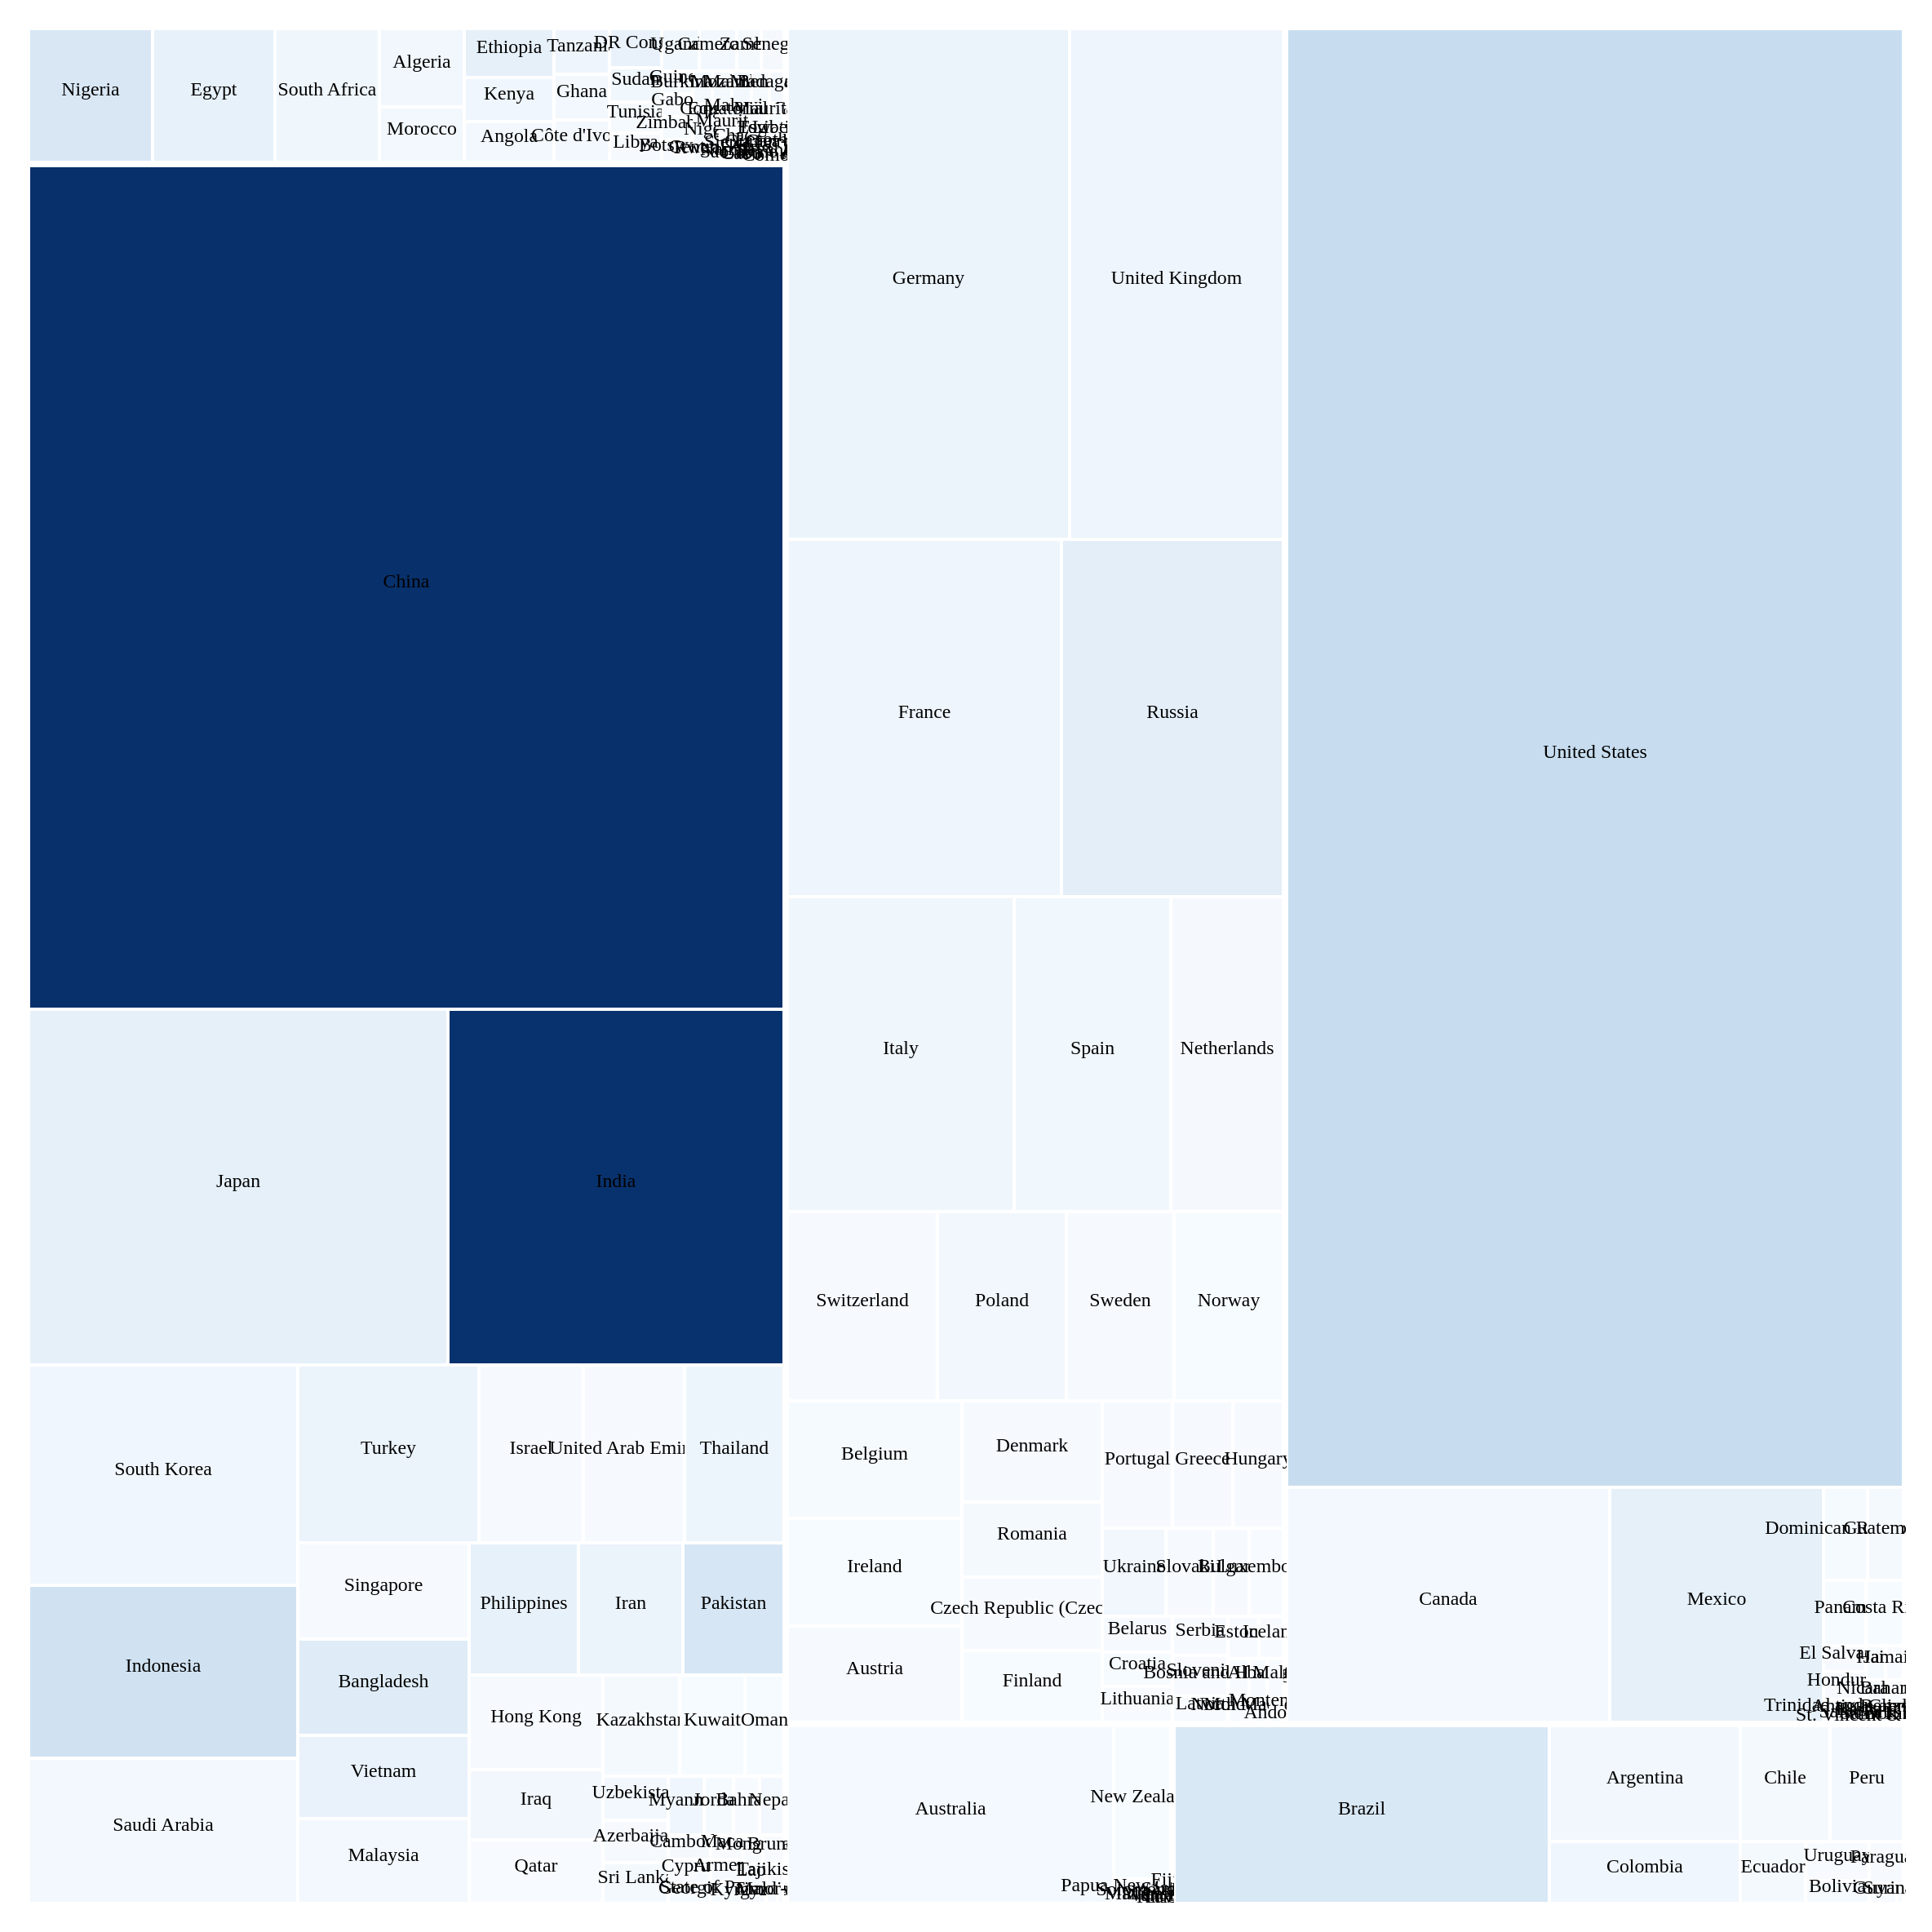
\includegraphics[height=3in, width=0.75\textwidth]{images_ashish/treemap2.png}
    \caption{Treemap 2}
    \label{fig_2}
\end{figure*}
\textbf{Treemap - II}\\
In this treemap (Figure \ref{fig_1})the countries are grouped on the basis of continents. The size of each rectangle in the treemap corresponds to the Gross Domestic Product (GDP) of the respective country. The color of each rectangle indicates the population of the corresponding country. \\
\underline{\textbf{Inferences}}\\
Population Density:  By combining GDP size and population color, we can assess the relationship between economic output and population, i.e  countries with higher GDPs also more populous, or are there variations in this relationship.\\
Wealth Distribution: We can observe how wealth (GDP) is distributed across continents and within each continent.\\
Identifying Economic Powerhouses: Countries like India and China with both large GDP and population sizes. These could be economic powerhouses that contribute significantly to both economic output and global demographic trends.\\
\begin{figure*}
\centering
    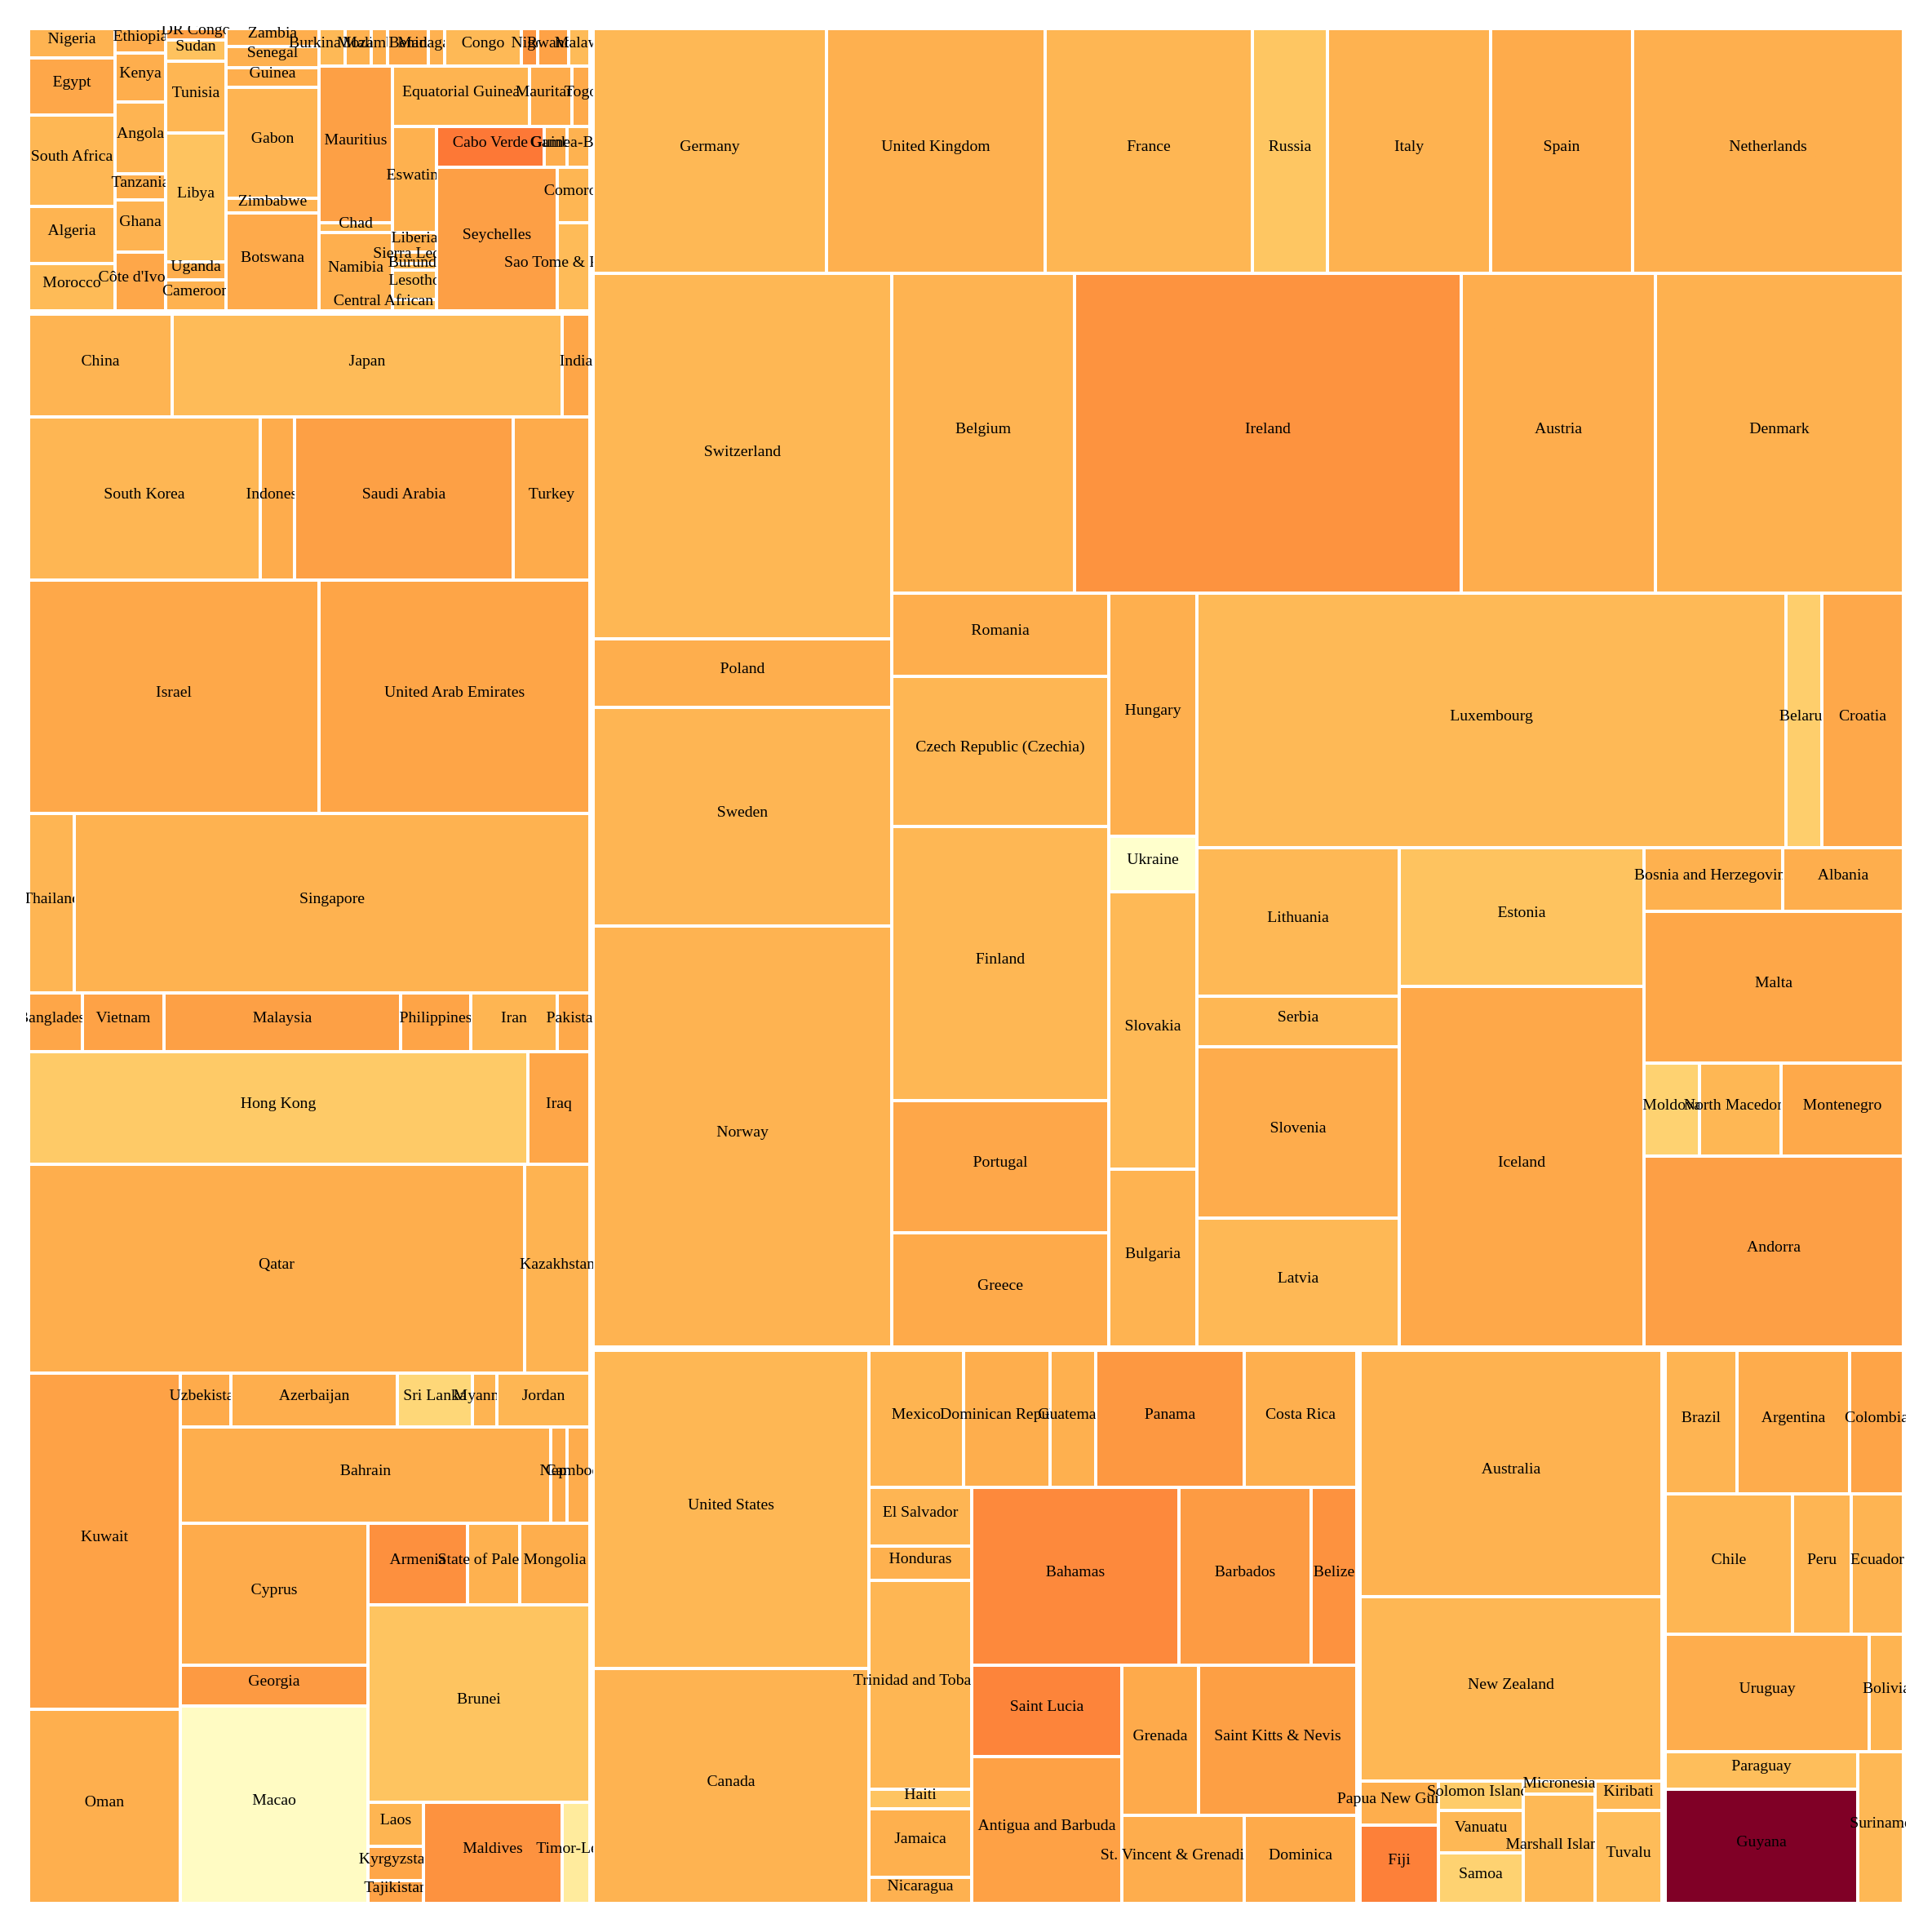
\includegraphics[height=3in, width=0.75\textwidth]{images_ashish/treemap3.png}
    \caption{Treemap 3}
    \label{fig_3}
\end{figure*}
\textbf{Treemap -III}\\
In this treemap, (Figure \ref{fig_3}) the countries are organised on the basis of continents. The size of each rectangle corresponds to the GDP Per Capita of the country and the color represents the GDP growth of that country for the year 2022.\\
\underline{\textbf{Inferences}}\\
Regional Economic Disparities: Larger rectangles would indicate higher GDP per capita, highlighting countries with higher individual income levels. Observe if there are significant differences in economic prosperity between continents.\\
Emerging Markets: Countries with smaller GDP per capita but high growth rates may represent emerging markets. These are areas where economic growth is significant, and there may be investment opportunities.\\
Stability Assessment: Observe if countries with higher GDP per capita tend to have more stable or lower growth rates. This can provide insights into the relationship between economic development and stability.\\
\begin{figure*}
\centering
    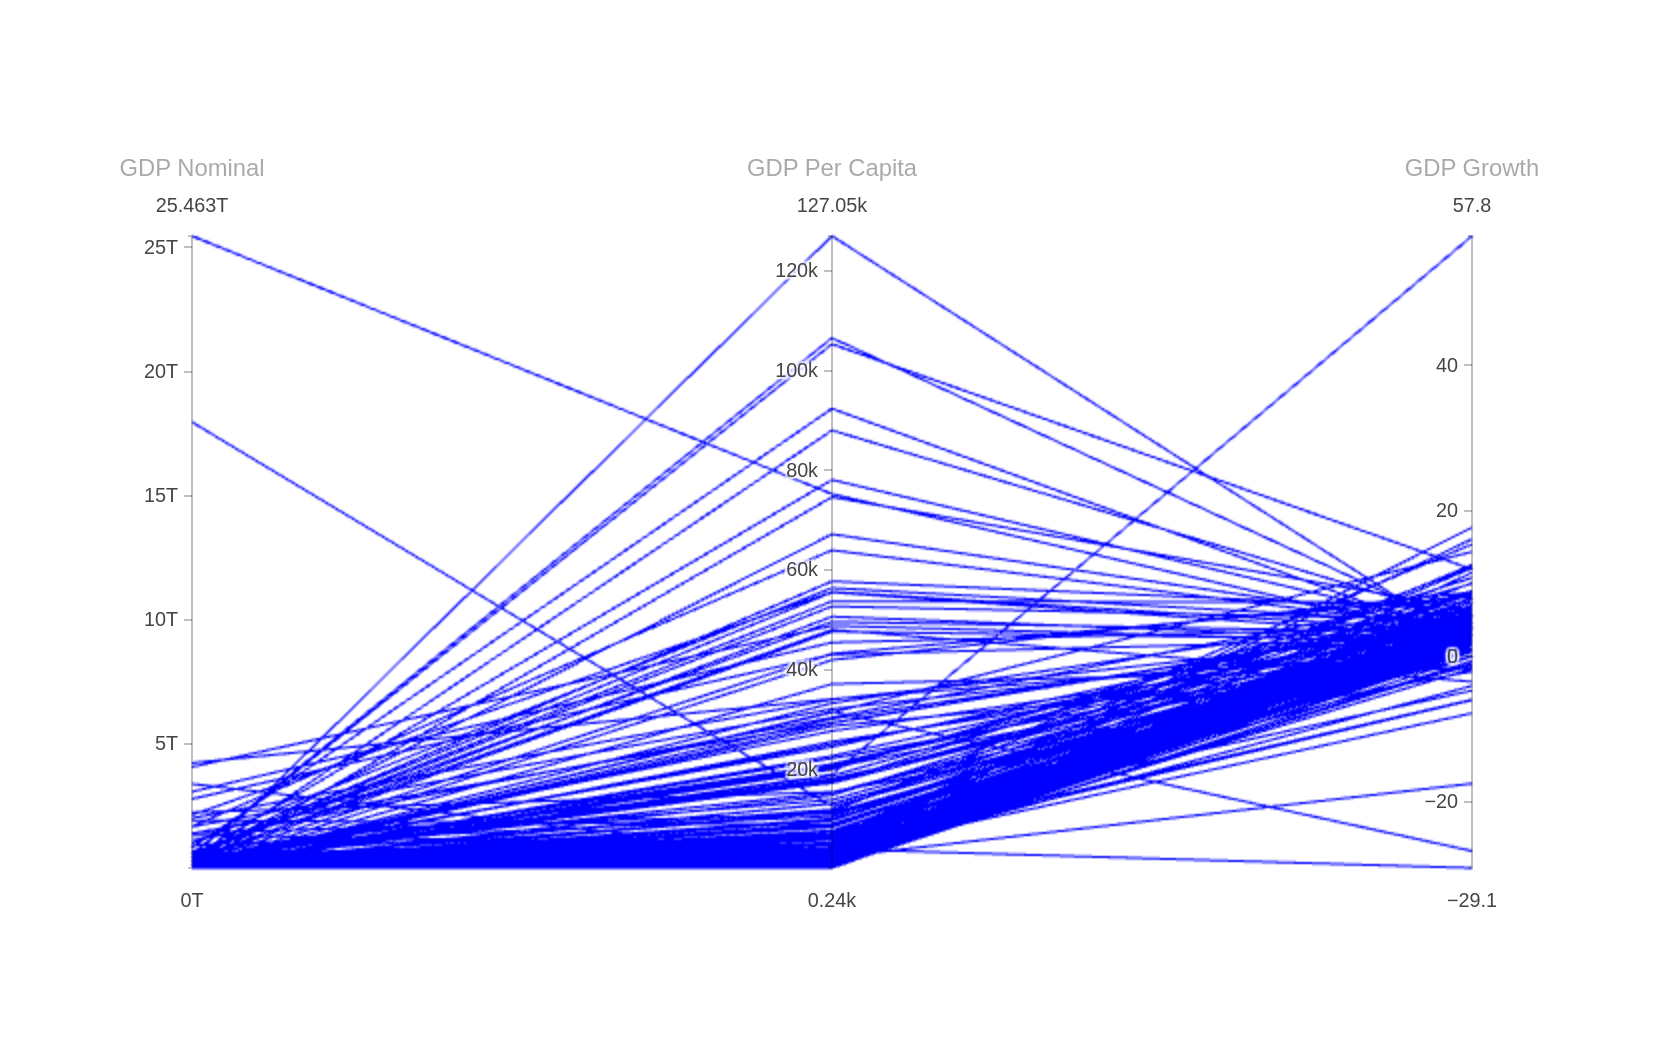
\includegraphics[height=3in, width=0.75\textwidth]{images_ashish/pcp_1.png}
    \caption{Parallel Coordinate Plot 1}
    \label{fig1}
\end{figure*}
\subsection{Parallel Coordinate Plot}
\textbf{Parallel Coordinate Plot - I}\\
In this plot (Figure \ref{fig1}) we have
Axes: In the order of the plot.
\begin{itemize}
    \item GDP\_Nominal Axis: Represents the GDP (Gross Domestic Product) of each country.
    \item GDP Per Capita Axis: Represents the GDP per capita for each country.
    \item GDP Growth Rate Axis: Represents the growth rate of GDP for each country. 
\end{itemize}
Lines:
\begin{itemize}
    \item Each country is represented by a line that connects points on these three axes.
    \item  The position of the line on each axis corresponds to the value of the respective variable for that country.
\end{itemize}
\underline{\textbf{Inferences}}
\begin{itemize}
    \item The first thing we notice is that some countries even though having high GDP Nominal have relatively less GDP per capita inferring that the economy is hugely dependent on its population or indicating a larger population.
    \item We also see countries whose GDP Nominal is pretty low but the  GDP per capita is sky rocketing indicating prosperous countries.
    \item Some countries had huge drop in their GDP growth rate (in order of -20\%) owing to the Ukraine Russia war.
\end{itemize}
\begin{figure*}
\centering
    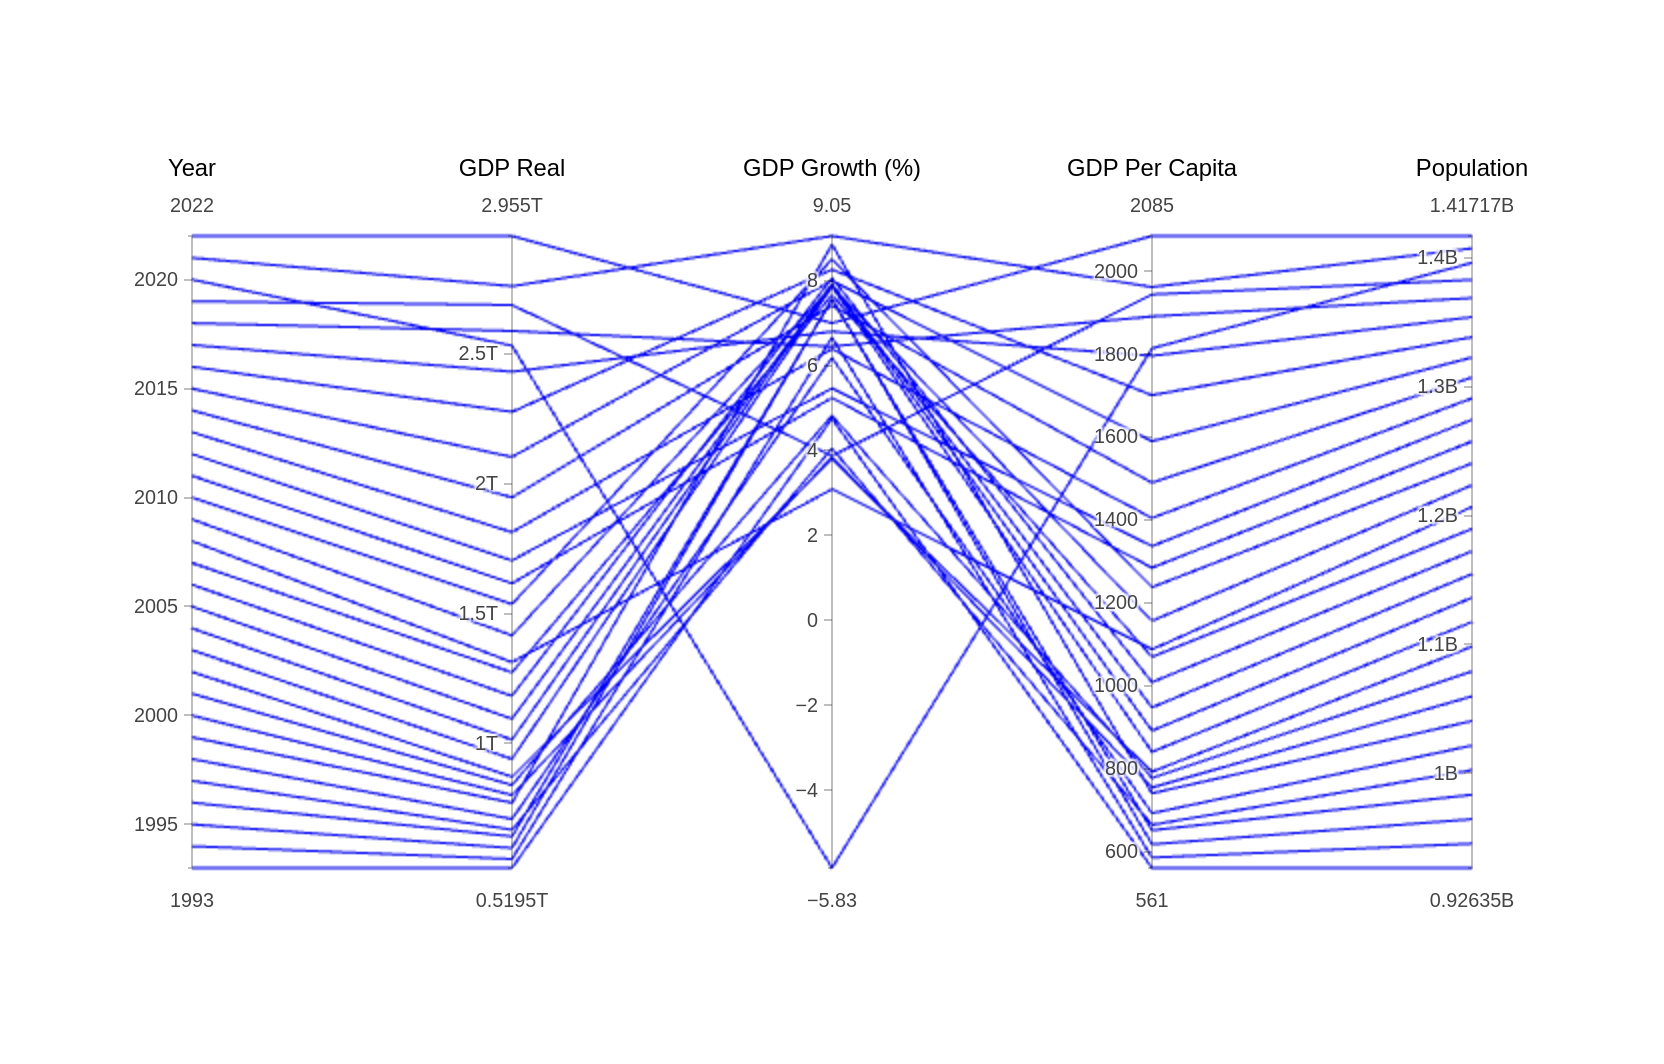
\includegraphics[height=3in, width=0.75\textwidth]{images_ashish/pcp_2.png}
    \caption{Parallel Coordinate Plot 2}
    \label{fig2}
\end{figure*}
 \textbf{Parallel Coordinate Plot -2}\\
The plot (Figure \ref{fig2}) consists of parallel axes, where each axis represents a different economic metric : Real GDP(inflated values), GDP Growth Rate , and GDP per capita and the Population.There are separate lines for each economic metric, connecting the values for each year.
\underline{\textbf{Inferences}}
\begin{itemize}
    \item We see that the GDP is increasing gradually as the time goes. We only have one outlier data i.e in the year 2021 when the world was hit by Covid-19 pandemic.
    \item When we reorder the axis and keep GDP Real and GDP per capita adjacent, we see that GDP per capita is increasing year to year even though populaiton is increasing. This infers that GDP growth rate is higher than population growth rate rather population growth rate is decreasing.
    \item Especially in 1990s we see a boom in economic growth of India verified huge GDP growth rates but that did not result in huge increase in the GDP per capita, owing to huge population of India.
\end{itemize} 
\begin{figure*}
\centering
    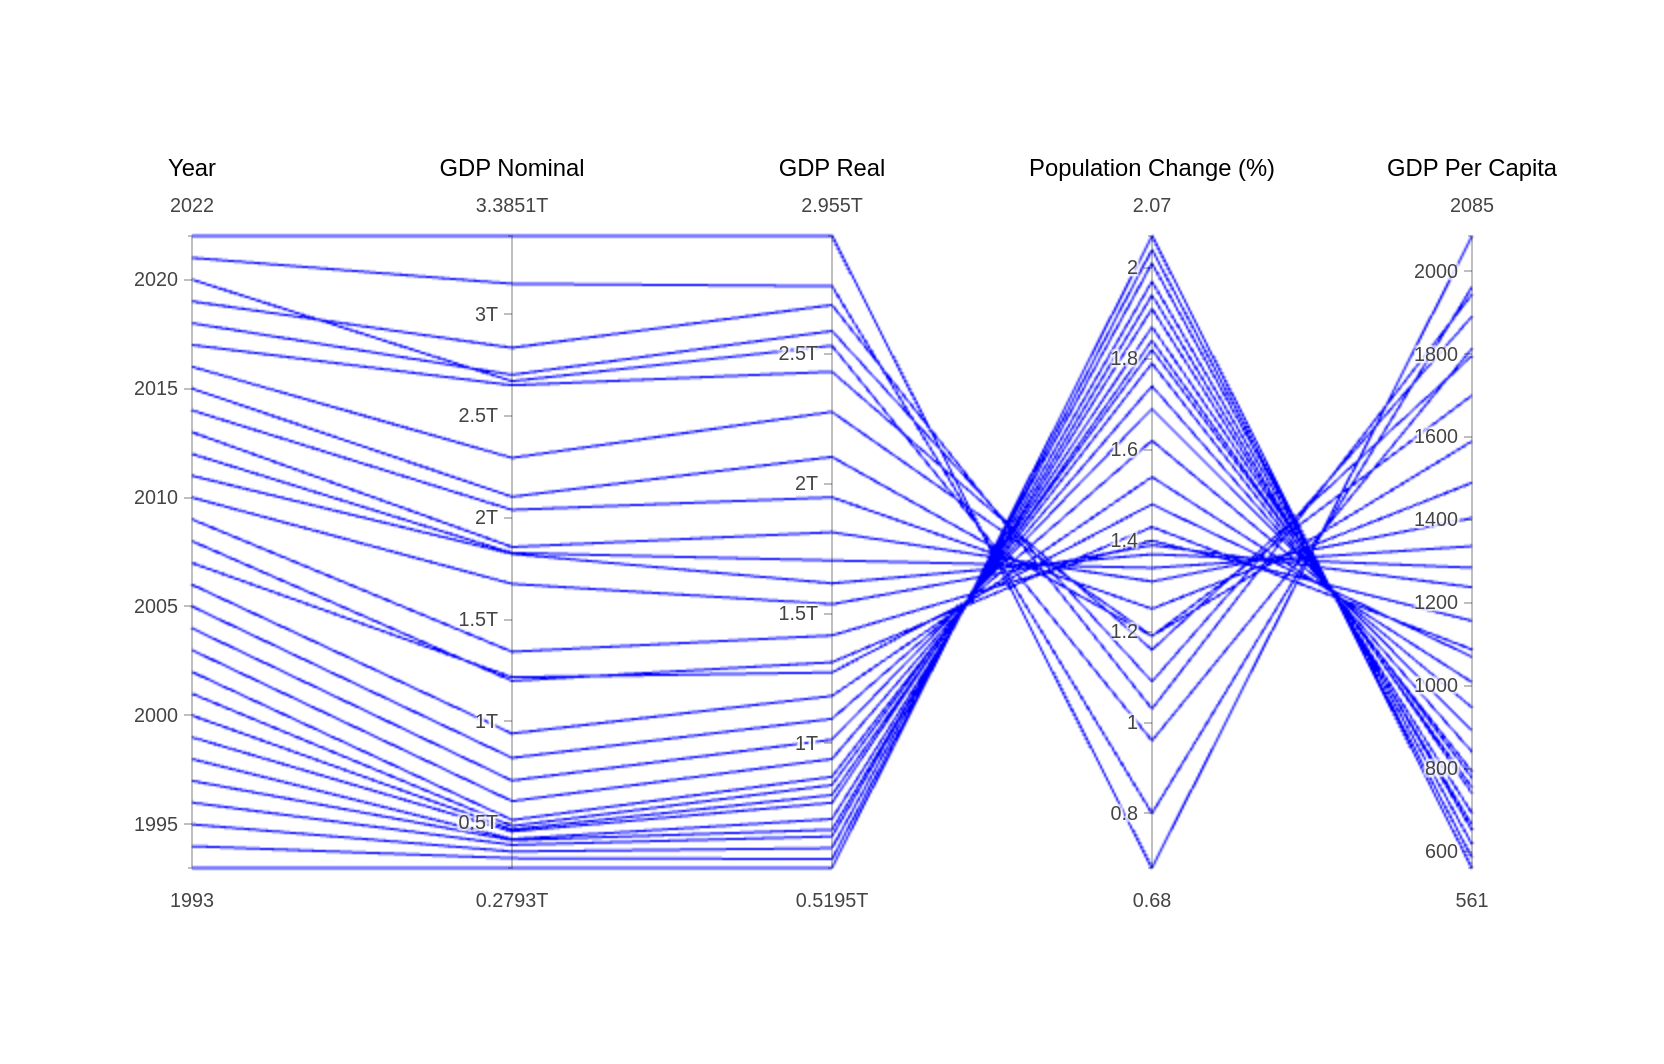
\includegraphics[height=3in, width=0.75\textwidth]{images_ashish/pcp_3.png}
    \caption{Parallel Coordinate Plot 3}
    \label{fig3}
\end{figure*}
\textbf{Parallel Coordinate Plot -3}\\
 A parallel coordinate plot (Figure \ref{fig3})  with axes representing Real GDP, Nominal GDP, GDP per capita, Population Change, and Year involves multiple parallel lines connecting values for each year across these economic metrics.
\underline{\textbf{Inferences}}
\begin{itemize}
    \item We see that the population growth rate was high during the early years but it started gradually decreasing as the time goes owing generation shift and mindset.
    \item We see a gradual increase in GDP Nominal and also GDP per capita showing that India is slowly becoming an economic powerhouse.
    \item As population growth rate got declining the GDP per capita increased due to ecomomic growth of India.
\end{itemize}


section*{Introduction}

A node-link diagram is a visual representation where nodes signify entities, and edges represent connections between them. This simple yet powerful tool provides a clear view of relationships within complex datasets. Node link diagrams also allows to represent different variables of the dataset via the attributes like color, size of node, thickness of edges etc and these little visual things make interpreting the data easier.

\section*{The Dataset}

Our dataset draws inspiration from George R. R. Martin's "A Song of Ice and Fire" series, covering books one to five. Each edge indicates that two characters are mentioned within fifteen words of each other. Edge multiplicities capture the frequency of these appearances, painting a vivid picture of the character interactions in Martin's intricate literary universe. This report explores the creation of a node-link diagram, employing different layout algorithms and sampling techniques to untangle the web of connections within this fictional social network.




\section*{Sampling Strategy}
The decision to use sampling in constructing the node-link diagram was driven by the dataset's size, leading to a cluttered diagram. With an abundance of edges and nodes, the challenge was to distill meaningful patterns.

To address this, a systematic sampling methodology was implemented. Initially, the total weight corresponding to each node was calculated by adding the weights of all the edges corresponding to that node.These weights facilitated the prioritization of nodes based on their overall influence within the network. Subsequently, the top 64 nodes having the highest total weights were selected. The new edged dataset included only those edges both of whose nodes were present in this list of 64 nodes.
Note that 64 was selected as it provided balance between including critical nodes and excluding non-critical nodes.

This strategy aimed to simplify the diagram while preserving the most influential nodes and their connections, offering a clearer view of the social network in "A Song of Ice and Fire."


% Add the images at the end of the section
\begin{figure}[h]
  \centering
  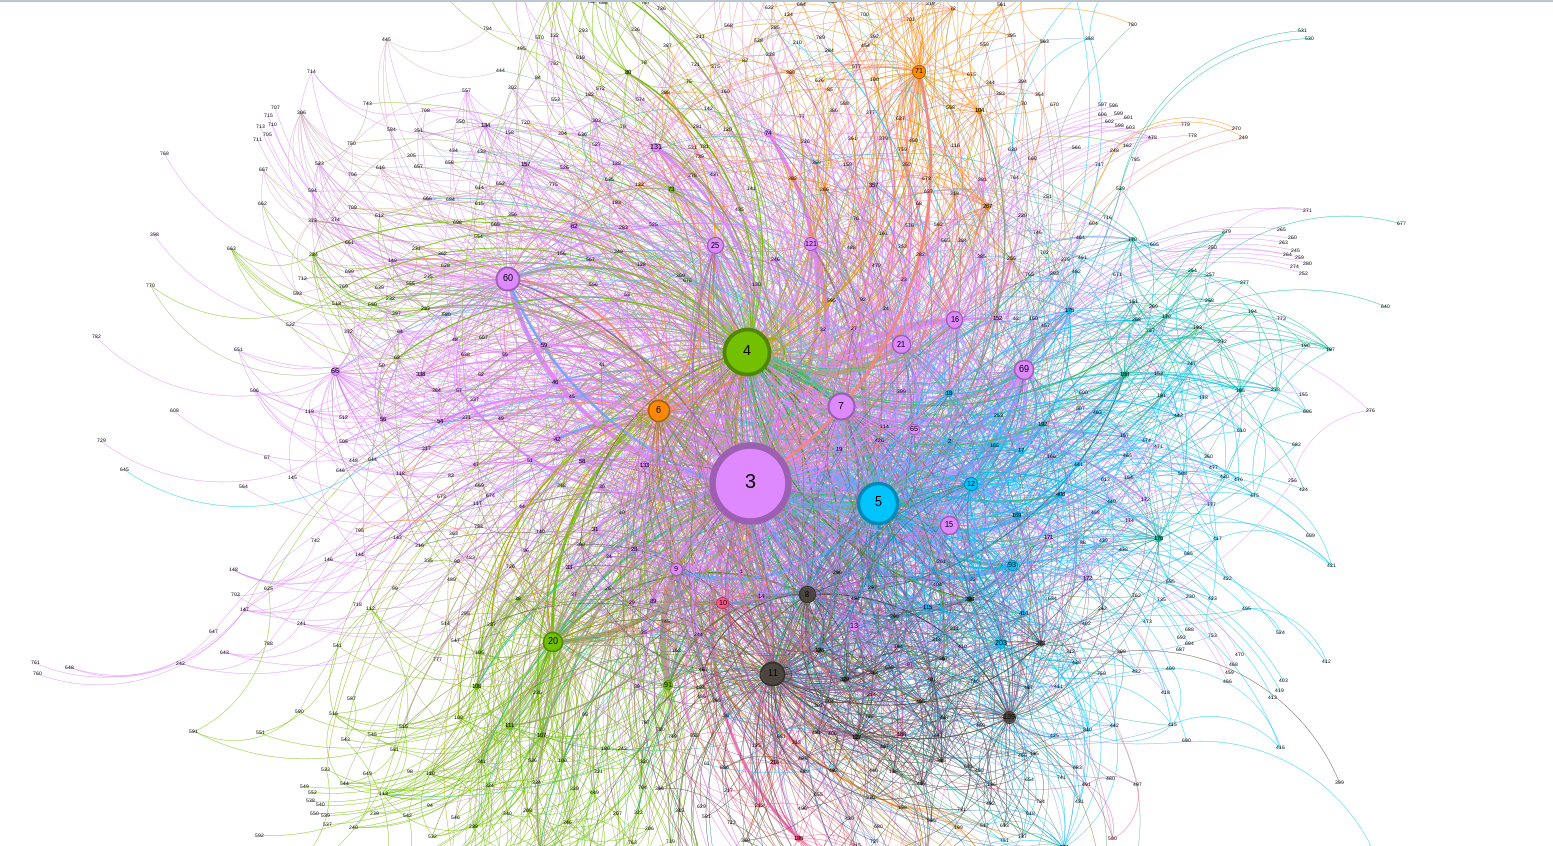
\includegraphics[width=0.7\linewidth]{./images_ricky/unsamples_forceAtlas2_withEdges.png}
  \caption{Node-Link Diagram Without Sampling}
  \label{fig:without_sampling}
\end{figure}

\begin{figure}[h]
  \centering
  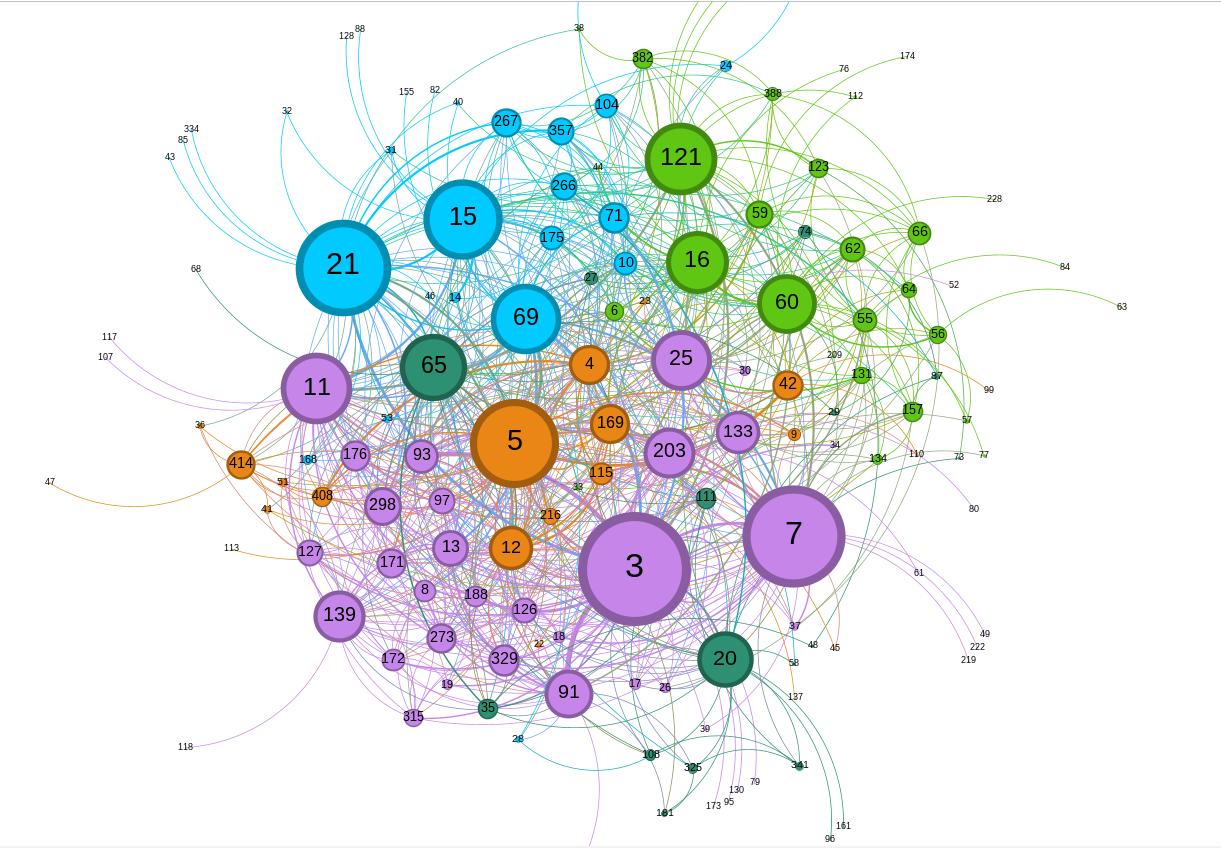
\includegraphics[width=0.7\linewidth]{./images_ricky/sampled__forceAtlas2_withEdges.png}
  \caption{Node-Link Diagram With Sampling}
  \label{fig:with_sampling}
\end{figure}



\section*{Layout Algorithms}

Two layout algorithms, \textit{forceAtlas2} and \textit{Fruchterman-Reingold}, were employed to visualize the node-link diagram. These algorithms play a crucial role in determining the spatial arrangement of nodes and edges within the graph.

\textbf{ForceAtlas2:} This algorithm simulates physical forces between nodes, aiming to achieve a balanced layout. It considers factors like repulsion between nodes and attraction along edges, dynamically adjusting positions to minimize overlapping and achieve an aesthetically pleasing arrangement.

\textbf{Fruchterman-Reingold:} Based on a physical analogy of attractive and repulsive forces, this algorithm strives to distribute nodes evenly across the visualization space. Nodes connected by edges exert attractive forces, while all nodes repel each other, leading to an equilibrium that represents the network's structure.

\vspace{0.8cm}

\textbf{NOTE : }
For all layouts used, the following parameters were kept common:

1. \textbf{Node Coloring:} The modularity statistic was employed to determine node colors, highlighting community structures within the network.

2. \textbf{Node Size and Labels:} The page rank statistic was utilized for both node sizes and labels, emphasizing the importance of nodes within the network.


\vspace{0.8cm}

Now, let's visualize the outcomes of these algorithms:

\begin{figure}[h]
  \centering
  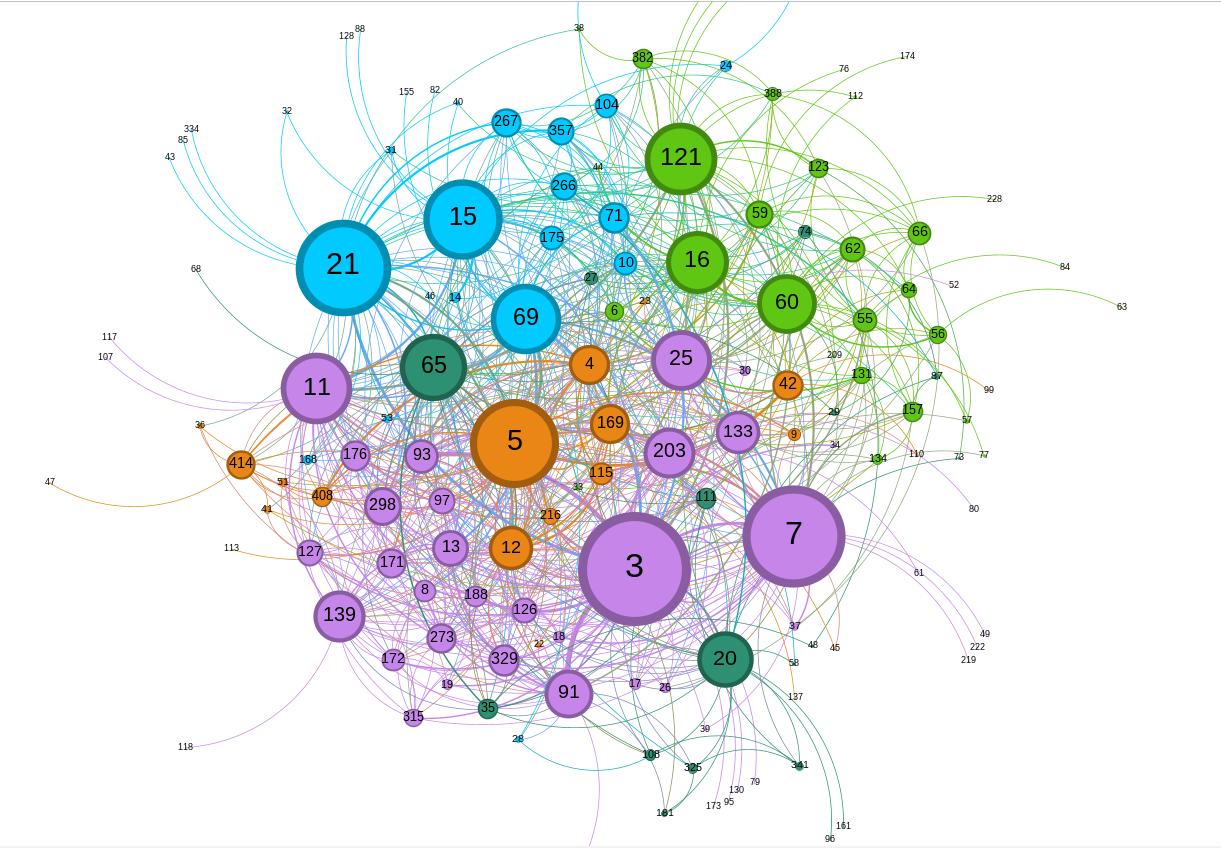
\includegraphics[width=0.7\linewidth]{./images_ricky/sampled__forceAtlas2_withEdges.png}
  \caption{ForceAtlas2 Layout with Edges}
  \label{fig:forceAtlas2_with_edges}
\end{figure}

\begin{figure}[h]
  \centering
  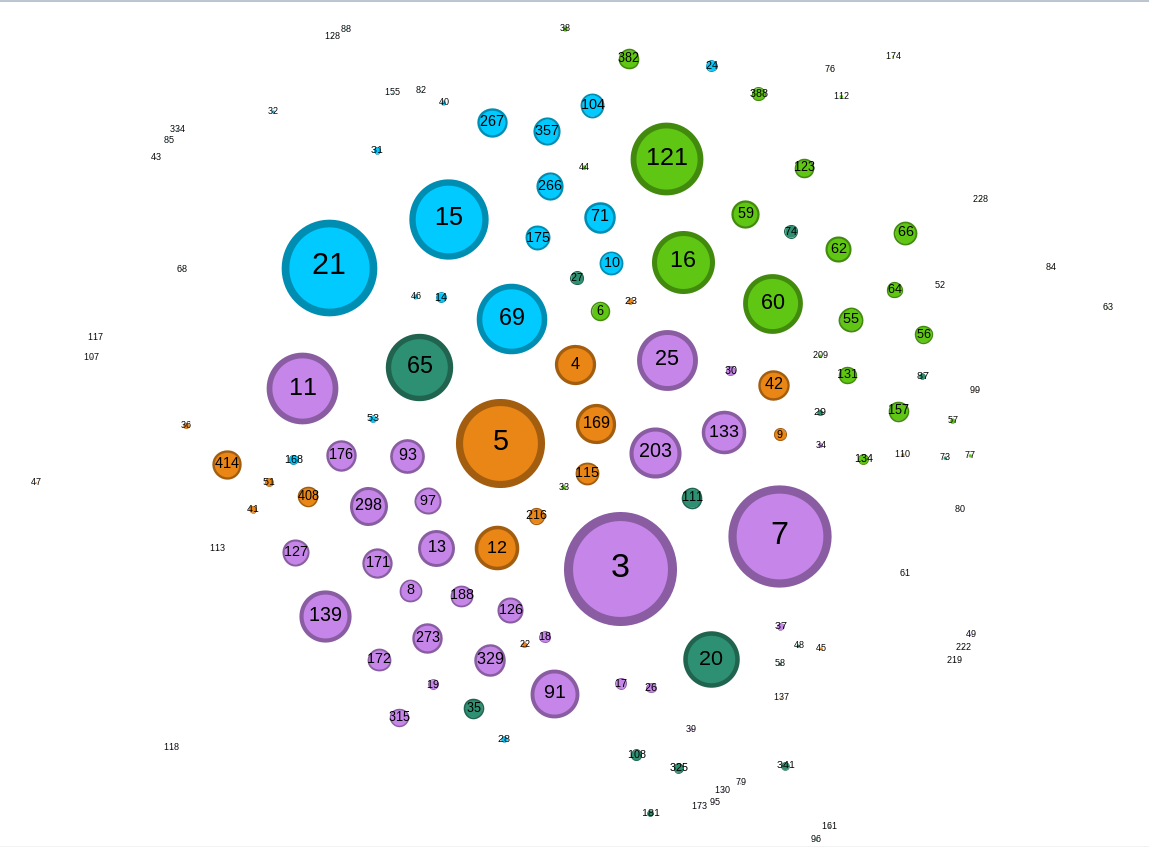
\includegraphics[width=0.7\linewidth]{./images_ricky/sampled_forceAtlas2_withoutEdges.png}
  \caption{ForceAtlas2 Layout Without Edges}
  \label{fig:forceAtlas2_without_edges}
\end{figure}

\begin{figure}[h]
  \centering
  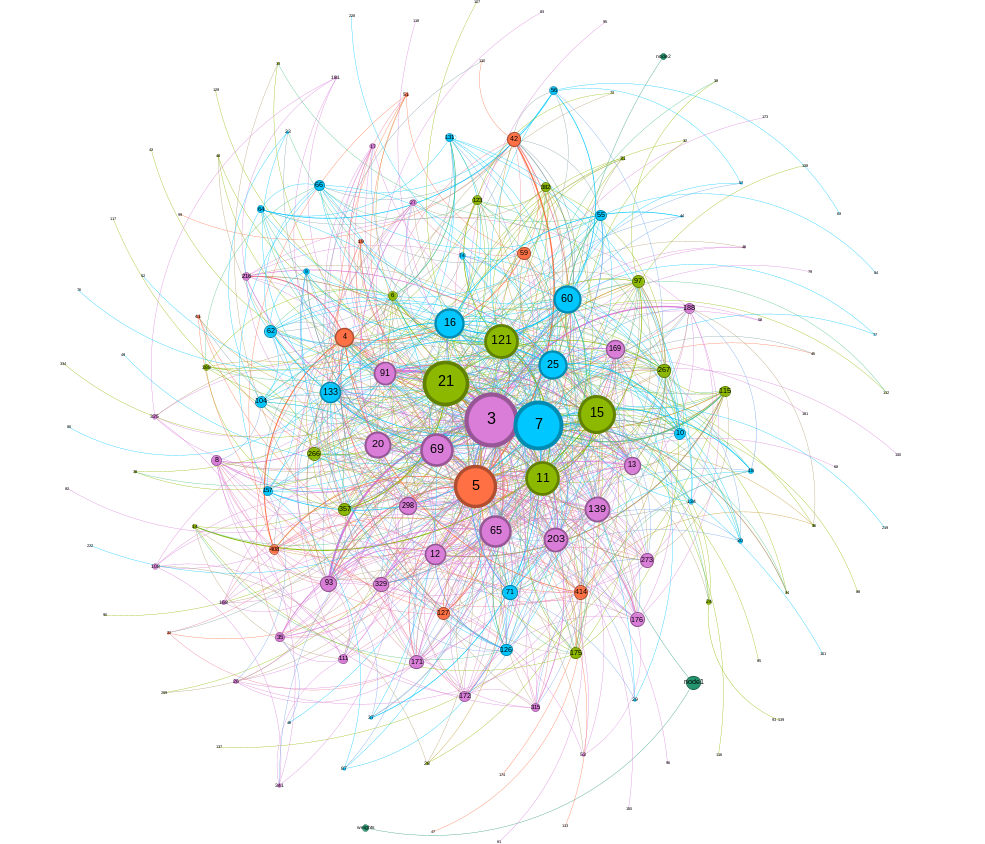
\includegraphics[width=0.7\linewidth]{./images_ricky/sampled_fruchterman_reingold_withEdges.png}
  \caption{Fruchterman-Reingold Layout with Edges}
  \label{fig:fruchterman_with_edges}
\end{figure}

\begin{figure}[h]
  \centering
  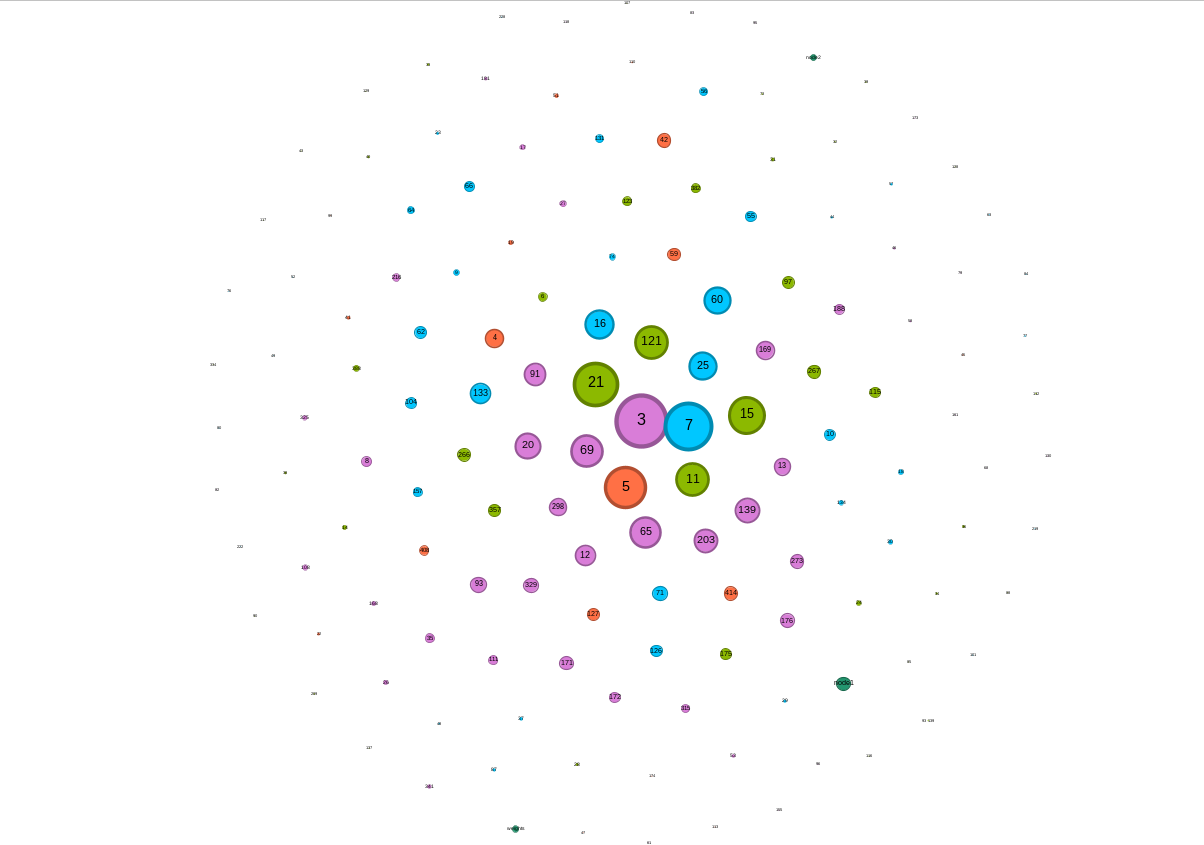
\includegraphics[width=0.7\linewidth]{./images_ricky/sampled_fruchterman_reingold_withoutEdges.png}
  \caption{Fruchterman-Reingold Layout Without Edges}
  \label{fig:fruchterman_without_edges}
\end{figure}


We can see from figures \ref{fig:fruchterman_with_edges} and \ref{fig:fruchterman_without_edges} that the outcome of Fruchterman-Reingold mostly has distributed the nodes based on the sizes( Although this is not how internally this algorithm works but for this case it's observed to be doing this)

We can see from figures \ref{fig:forceAtlas2_with_edges} and \ref{fig:forceAtlas2_without_edges} that the outcome of ForceAtlas2 algorithm has mostly gatherd the nodes which has many edges togather and it makes it look like clusters of different colors are being formed too.( Although this is not how internally this algorithm works but for this case it's observed to be doing this)


\end{document}
